\pdfoutput=1
\documentclass[a4paper,onecolumn,11pt,unpublished,nopdfoutputerror]{quantumarticle}

\usepackage[utf8]{inputenc}
\usepackage[T1]{fontenc}
\usepackage{amsmath,amssymb,amsthm,mathtools}
\usepackage{booktabs,array,multirow,longtable,float}
\usepackage{enumitem}
\usepackage{xcolor}
\usepackage{tikz}
\usetikzlibrary{positioning,arrows.meta,calc,shapes.geometric,backgrounds,fit}
\usepackage{pgfplots}
\pgfplotsset{compat=1.17}
\usepackage[most]{tcolorbox}
\usepackage{microtype}
\usepackage{xurl}
\usepackage{hyperref}
\usepackage[capitalise,noabbrev]{cleveref}

%% ---- macros.tex ----
% ---------------------------------------------------------------- theorem environments
\newtheorem{theorem}{Theorem}[section]
\newtheorem{lemma}[theorem]{Lemma}
\newtheorem{proposition}[theorem]{Proposition}
\newtheorem{corollary}[theorem]{Corollary}
\newtheorem{conjecture}[theorem]{Conjecture}
\theoremstyle{definition}
\newtheorem{definition}[theorem]{Definition}
\newtheorem{example}[theorem]{Example}
\newtheorem{remark}[theorem]{Remark}
\newtheorem{question}[theorem]{Question}

\crefname{conjecture}{Conjecture}{Conjectures}
\crefname{question}{Question}{Questions}

% ---------------------------------------------------------------- colours
\definecolor{leangreen}{HTML}{1B7F5B}
\definecolor{certblue}{HTML}{2A5DB0}
\definecolor{numorange}{HTML}{B35C00}
\definecolor{softgray}{HTML}{F4F4F1}
\definecolor{inkgray}{HTML}{55585E}

% ---------------------------------------------------------------- status tags
% \lean{name}   : the statement is a theorem of the Lean development (kernel-checked)
% \leanc{name}  : the Lean proof uses a native_decide finite computation
% \cert{X1}     : a finite fact re-checked by the independent Python checker
% \paperonly    : proved in this paper, not (yet) formalised
\newcommand{\leantagbox}[2]{\unskip\nobreak\hfill\penalty50\hskip1em\null\nobreak\hfill
  {\footnotesize\color{leangreen}\textsf{#1}~\texttt{\hyphenchar\font=-1 #2}}}
\newcommand{\lean}[1]{\leantagbox{Lean\,\ding:}{#1}}
\newcommand{\leanc}[1]{\leantagbox{Lean\,$\ast$:}{#1}}
\newcommand{\leanin}[1]{{\footnotesize\color{leangreen}[\textsf{Lean}:~\texttt{#1}]}}
\newcommand{\leancin}[1]{{\footnotesize\color{leangreen}[\textsf{Lean}\,$\ast$:~\texttt{#1}]}}
\newcommand{\cert}[1]{\textcolor{certblue}{\textsf{[#1]}}}
\newcommand{\paperonly}{\unskip\nobreak\hfill\penalty50\hskip1em\null\nobreak\hfill{\footnotesize\color{inkgray}\textsf{paper proof}}}
\newcommand{\ding}{\ensuremath{\checkmark}}
\newcommand{\lname}[1]{\texttt{\textcolor{leangreen}{#1}}}

% ---------------------------------------------------------------- maths
\newcommand{\F}{\mathbb{F}_2}
\newcommand{\C}{\mathbb{C}}
\newcommand{\R}{\mathbb{R}}
\newcommand{\Z}{\mathbb{Z}}
\newcommand{\N}{\mathbb{N}}
\renewcommand{\deg}{\operatorname{deg}}
\newcommand{\Lines}{\mathcal{L}}
\newcommand{\Pts}{\mathcal{P}}
\newcommand{\im}{\operatorname{Im}}
\newcommand{\rad}{\operatorname{rad}}
\newcommand{\tr}{\operatorname{tr}}
\newcommand{\sgn}{\operatorname{sgn}}
\newcommand{\Sp}{\operatorname{Sp}}
\newcommand{\Orth}{\operatorname{O}}
\newcommand{\Aut}{\operatorname{Aut}}
\newcommand{\supp}{\operatorname{supp}}
\newcommand{\viol}{\operatorname{viol}}
\newcommand{\OPT}{\mathrm{OPT}}
\newcommand{\E}{\mathbb{E}}
\newcommand{\Var}{\operatorname{Var}}
\newcommand{\W}[1]{W(#1,2)}
\newcommand{\Qp}[1]{Q^{+}(#1,2)}
\newcommand{\Qm}[1]{Q^{-}(#1,2)}
\newcommand{\ket}[1]{\lvert #1\rangle}
\newcommand{\bra}[1]{\langle #1\rvert}
\newcommand{\braket}[2]{\langle #1\vert #2\rangle}
\newcommand{\ev}[1]{\langle #1\rangle}
\newcommand{\proj}[1]{\lvert #1\rangle\langle #1\rvert}
\newcommand{\Vs}{V^{\ast}}
\newcommand{\eps}{\varepsilon}
\newcommand{\ind}[1]{[\![#1]\!]}

% ---------------------------------------------------------------- repository (placeholder: change once public)
\newcommand{\repourl}{https://github.com/WordsonRobert/pauli_contextuality}
\newcommand{\repo}{\href{\repourl}{\nolinkurl{github.com/WordsonRobert/pauli_contextuality}}}

% ---------------------------------------------------------------- boxes
\newtcolorbox{summarybox}[1][]{enhanced,breakable,colback=softgray,colframe=softgray,
  boxrule=0pt,arc=2pt,left=8pt,right=8pt,top=6pt,bottom=6pt,#1}

% ---------------------------------------------------------------- Lean listings
\usepackage{listings}
\lstdefinelanguage{lean4}{
  morekeywords={def,theorem,lemma,structure,where,noncomputable,abbrev,fun,by,if,then,else,let,have,show,
    namespace,end,open,import,instance,Prop,Type,with,match,at},
  sensitive=true,
  morecomment=[l]{--},
  morecomment=[s]{/-}{-/},
  morestring=[b]",
}
\lstset{language=lean4,basicstyle=\ttfamily\footnotesize,keywordstyle=\color{leangreen}\bfseries,
  commentstyle=\color{inkgray}\itshape,columns=fullflexible,keepspaces=true,
  backgroundcolor=\color{softgray},frame=none,xleftmargin=6pt,xrightmargin=6pt,
  aboveskip=6pt,belowskip=6pt,breaklines=true,
  extendedchars=true,
  literate=
   {∑}{{$\sum$}}1 {∈}{{$\in$}}1 {∉}{{$\notin$}}1 {≤}{{$\le$}}1 {≥}{{$\ge$}}1 {≠}{{$\ne$}}1
   {→}{{$\to$}}1 {↔}{{$\leftrightarrow$}}1 {∀}{{$\forall$}}1 {∃}{{$\exists$}}1 {∧}{{$\wedge$}}1
   {ℕ}{{$\mathbb N$}}1 {ℝ}{{$\mathbb R$}}1 {ℂ}{{$\mathbb C$}}1 {ℚ}{{$\mathbb Q$}}1
   {⟨}{{$\langle$}}1 {⟩}{{$\rangle$}}1 {α}{{$\alpha$}}1 {γ}{{$\gamma$}}1 {𝓝}{{$\mathcal N$}}1
   {·}{{$\cdot$}}1 {×}{{$\times$}}1 {₀}{{$_0$}}1 {ᵀ}{{$^{\mathsf T}$}}1
}

\setlength{\emergencystretch}{2.5em}

\begin{document}

\title{Almost half wrong: the contextuality degree of multi-qubit Pauli configurations}

\author{Wordson}
\affiliation{Department of Mathematics and Statistics, Indian Institute of Science Education and Research Kolkata, Mohanpur 741246, India}
\orcid{0009-0001-7340-5530}

\author{Savith A}
\affiliation{Indian Institute of Science Education and Research Kolkata, Mohanpur 741246, India}

\author{C.~Jerin Mahibha}
\affiliation{Meenakshi Sundararajan Engineering College, Chennai, India}

\maketitle

%% ---- sec-abstract.tex ----
\begin{abstract}
Take a set of multi-qubit Pauli observables and call a triple of them a context when they commute and multiply to
$\pm I$. A noncontextual hidden-variable model must give every observable a fixed value $\pm1$, and then some
contexts come out with the wrong product. The \emph{contextuality degree} is the smallest possible number of such
wrong contexts. We study it for general configurations and for the classical finite geometries: the symplectic
polar space $\W{2N-1}$ of all $N$-qubit Paulis and its quadrics.

The central tool is an exact identity: the degree equals half the number of contexts minus the largest cubic
trace $\tr(M_g^3)/(12\cdot2^N)$ of a signed sum $M_g=\sum_a g(a)P_a$ of the observables. One positive-semidefinite
trace inequality turns it into a lower bound, and random states turn it into an upper bound. Together they show
that the contextuality ratio $\rho_N=\deg\W{2N-1}/|\Lines|$ tends to $\tfrac12$, with
$\tfrac12-\rho_N=\Theta(2^{-N/2})$. Put plainly, for many qubits every noncontextual model gets almost half of the
contexts wrong, and this is the most any model can be forced to get wrong. The bound is exact precisely when some
pure state has Pauli expectations of constant modulus on the configuration and zero off it. On three qubits these
are the Hoggar SIC fiducials, so the optimal noncontextual assignments of the three-qubit space are exactly the
sign patterns of maximally magic states. The same mechanism gives a short proof that the four-qubit hyperbolic
quadric has degree $315$ and a new exactly solved five-qubit configuration of degree $480$.

Read as a two-player game, a configuration becomes a linear-system nonlocal game whose classical value is
$1-\deg/(3|\Lines|)$ and whose quantum value is $1$ with $N$ EPR pairs. The symplectic family has classical value
tending to $\tfrac56$, the minimum possible for any such game, and we give the matching dimension--gap law.

We also prove that computing the degree is NP-hard even for induced configurations, that all hard instances are
exponentially sparse in a spectral sense while dense ones are easy, a transfer and rigidity theory for symmetric
geometries, exact degrees of all subspace sections, $\deg\Qm7\ge216$ by an elementary certificate, and new lower
bounds for every $N\ge4$. Almost all of this is formalised in Lean~4 with Mathlib: about $1{,}100$ machine-checked
theorems, with every finite computation isolated and audited.
\end{abstract}


\tableofcontents

%% ---- sec-intro.tex ----
%=====================================================================================================
\section{Introduction}\label{sec:intro}
%=====================================================================================================

The Peres--Mermin square is nine two-qubit Pauli observables arranged in a $3\times3$ grid. Every row and every
column consists of commuting observables, and the product along each line is $+I$, except along one column,
where it is $-I$. Try to give each observable a predetermined value $\pm1$ that respects all six products: the
product of all row constraints and the product of all column constraints use every observable twice, so they
must agree, and they do not. At least one of the six constraints must fail. This is the Kochen--Specker theorem
in its smallest Pauli form~\cite{KochenSpecker1967,Peres1990,Mermin1990}.

The obvious next question is quantitative. Given a larger set of Pauli observables, how many of its constraints
must a noncontextual assignment break? De~Boutray, Holweck, Giorgetti, Masson and Saniga~\cite{deBoutray2022}
named this number the \emph{contextuality degree}. It has a clean operational reading: summing the signed context
correlators gives a state-independent inequality whose noncontextual bound is the number of contexts $m$ minus
twice the degree, while quantum mechanics reaches $m$ in every state (\cref{prop:operational}). The degree is
therefore half of the classical--quantum gap of the parity test, and it fixes the visibility at which uniformly
attenuated data stop violating it.

Computing degrees has been a mostly numerical affair. For two and three qubits the values are known by SAT
solving~\cite{deBoutray2022,Muller2024}, and the optimal unsatisfied sets have a beautiful description through
split Cayley hexagons~\cite{Saniga2023}. For four to six qubits there are heuristic upper bounds and much weaker
lower bounds~\cite{Muller2024heur}; Li, Gupta and Ganesh recently proved $\deg\Qp7=315$ with a SAT-certified
classification~\cite{LiGuptaGanesh2026}. What was missing is any argument that works for all $N$ at once. Is the
fraction of violated contexts bounded away from $\tfrac12$? Does it grow? How fast? Which configurations are the
most contextual, and why are the three-qubit numbers so clean?

\subsection{What we prove}

\paragraph{An identity and a limit (\cref{sec:spectral,sec:asymptotics}).} For any \emph{induced} configuration
$X$, meaning a set of Pauli labels together with all of the contexts it contains, and any assignment
$g:X\to\{\pm1\}$, the number of violated contexts is
\[
  \viol(g)\;=\;\frac{|\Lines_X|}{2}\;-\;\frac{\tr\bigl(M_g^3\bigr)}{12\cdot2^N},\qquad M_g=\sum_{a\in X}g(a)P_a.
\]
This is \cref{thm:trace}. Bounding the largest eigenvalue of $M_g$ by Cauchy--Schwarz and Pauli completeness, and
then a cubic trace by one positive-semidefinite trace inequality, gives a lower bound on the degree of every
induced configuration (\cref{thm:spectral}). Choosing $g$ as the sign pattern of a random state gives an upper
bound. For the full symplectic polar space the two meet up to a constant:
\[
  0.255\cdot2^{-N/2}\;\le\;\tfrac12-\rho_N\;\le\;2^{-N/2}\qquad(N\ge7),\qquad\text{so}\quad\rho_N\to\tfrac12
\]
(\cref{thm:limit,thm:rate}), and the lower constant improves to $(2/\pi)^{3/2}\approx0.508$ asymptotically
(\cref{thm:kendall}). The sequence $\rho_N$ is non-decreasing, strictly increasing for $3\le N\le11$, and has a
strict jump in every window of four steps from $N=7$ on (\cref{thm:jumps}). Along the way the spectral bound
gives new lower bounds for every $N\ge4$, for instance $\deg\W7\ge1451$ and $\deg\W9\ge28786$, improving the
previous $1071$ and $17391$.

\paragraph{When the bound is exact: flat magic states (\cref{sec:tight}).} The spectral bound is attained if and
only if some pure state has $|\ev{P_a}|$ constant on $X$ and $\ev{P_a}=0$ for every other non-identity Pauli; the
optimal assignments are then exactly the sign patterns of such states (\cref{thm:tight}). For $X=\W5$ the states are
the fiducials of the Pauli-covariant SICs on three qubits (the Hoggar lines), and the optimal assignments of $\W5$
are in bijection with the fiducial projectors (\cref{thm:hoggar}). Since such SICs exist only for one and three
qubits, the bound for $\W{2N-1}$ is never exact for $N\ge4$. For the four-qubit hyperbolic quadric the flat state
is the real vector $\ket{+}^{\otimes4}-\ket{0}^{\otimes4}$ up to normalisation, which gives a two-line proof of
$\deg\Qp7=315$. We also find a five-qubit configuration of $496$ observables and $10880$ contexts with degree exactly
$480$. The flat states appearing here are the ones found by Cie\'sli\'nski in a study of maximal
magic~\cite{Cieslinski2026}; our theorem explains what they compute.

\paragraph{Games (\cref{sec:games}).} Every configuration defines a linear-system game in the sense of Cleve and
Mittal~\cite{CleveMittal2014}. Its classical value is exactly $1-\deg/(3|\Lines|)$ and its quantum value is $1$,
reached with $N$ EPR pairs and Pauli measurements. For the symplectic family the classical value tends to
$\tfrac56$, the smallest value any game of this format can have, and the gap behaves as
$\tfrac16-\Theta(2^{-N/2})$ for $N$-qubit Pauli strategies. A sampling argument turns this into a test with a
number of rounds independent of $N$.

\paragraph{Symmetry, small geometries and exact sections (\cref{sec:transfer,sec:geometry}).} A transfer theorem
says that the ratio of a line-transitive geometry dominates the ratio of everything embeddable in it, with
equality exactly when optimal assignments are tight on every translate. We add stability and multi-orbit
versions, show that fractional packings of local witnesses can never beat transfer, and compute the degree of
every subspace section of $\W{2N-1}$ and of the quadrics in terms of the full spaces. For the elliptic quadric we
prove $\deg\Qm7\ge216$ with an elementary certificate built only from odd grids and covering counts, and we
explain why the spectral method cannot go beyond $297$ there.

\paragraph{Complexity (\cref{sec:hardness}).} Computing the degree is NP-complete, also for induced configurations
and also for real observables; for induced configurations it is NP-hard to approximate within $2-\delta$, and for
sub-configurations of a quadric within any constant, with W[1]-hardness in the parameter. The spectral identity
adds a density dichotomy: on families whose spectral density grows the degree is trivially approximable, and the
hard instances we construct have exponentially small density.

\paragraph{Formalisation (\cref{sec:lean}).} Every theorem above whose proof is algebraic or combinatorial has been
proved in Lean~4 with Mathlib, starting from a definition of Pauli matrices as explicit complex matrices. The
development has $48$ modules and about $1{,}100$ theorems. Finite facts are checked by \texttt{native\_decide};
an axiom audit lists, for each of $270$ headline theorems, whether it depends on such a computation. The
remaining items (the continuous-probability parts of the rate, and the operational statements about noise) have
paper proofs here.

\begin{summarybox}
\textbf{How to read the status tags.} A theorem marked \textcolor{leangreen}{\textsf{Lean\,\ding:}\,\texttt{name}}
is a theorem of the Lean development whose axioms are only the standard ones (\texttt{propext},
\texttt{Classical.choice}, \texttt{Quot.sound}). The mark \textcolor{leangreen}{\textsf{Lean\,$\ast$:}\,\texttt{name}}
means that the Lean proof also trusts a finite computation evaluated by \texttt{native\_decide}. The mark
\textcolor{inkgray}{\textsf{paper proof}} means that the proof is given here and has not been formalised. Labels
such as \cert{X5} refer to an independent Python checker that recomputes every finite fact from scratch
(\cref{app:cert}). Code, certificates and the Lean sources are at \repo.
\end{summarybox}

\begin{table}[t]
\centering\small
\renewcommand{\arraystretch}{1.12}
\begin{tabular}{@{}llll@{}}
\toprule
configuration & lines & degree (this paper) & previously known\\\midrule
$\W3$ (doily) & 15 & $3$ & $3$~\cite{deBoutray2022}\\
$\W5$ & 315 & $63$, spectral one-liner; optimal $\leftrightarrow$ Hoggar SICs & $63$~\cite{Muller2024}\\
$\Qp7$ & 1575 & $315$, two-line spectral proof & $315$~\cite{LiGuptaGanesh2026}\\
$\Qm7$ & 1071 & $[\mathbf{216},315]$ & $[215,315]$~\cite{LiGuptaGanesh2026}\\
$\W7$ & 5355 & $[\mathbf{1451},1575]$ & $[1071,1575]$~\cite{Muller2024heur}\\
$\Qp9$ & 23715 & $[\mathbf{6426},6975]$ & $\le6975$~\cite{Muller2024heur}\\
$\Qm9$ & 19635 & $[\mathbf{4873},7087]$ & $\le7087$~\cite{Muller2024heur}\\
$\W9$ & 86955 & $[\mathbf{28786},31479]$ & $[17391,31479]$~\cite{Muller2024heur}\\
$X_{496}$ (5 qubits, new) & 10880 & $\mathbf{480}$ exactly & --\\
$\W{2N-1}$, all $N$ & $\tfrac{(4^N-1)(4^N-4)}{12}$ & $\bigl(\tfrac12-\Theta(2^{-N/2})\bigr)|\Lines|$ & --\\\bottomrule
\end{tabular}
\caption{Degrees of the main geometries. Bold entries are new lower bounds or exact values. All upper bounds for
four and five qubits are explicit assignments; those for $\W7$, $\Qp9$, $\Qm9$ and $\W9$ coincide with the
heuristic values of Muller et al.~\cite{Muller2024heur}, which our independent searches reproduce.}
\label{tab:headline}
\end{table}

\subsection{Related work}

\emph{The degree.} The invariant was introduced and computed by SAT for small quadrics and polar spaces
in~\cite{deBoutray2022}, refined in~\cite{Muller2024}, and estimated heuristically up to six qubits
in~\cite{Muller2024heur}. Muller and Giorgetti showed that it is determined by incidences and commutations
alone~\cite{MullerGiorgetti2025}; our cycle-sign lemma (\cref{lem:cyclesign}) gives a short proof of this.
The three-qubit optimal sets are governed by split Cayley hexagons~\cite{Saniga2023}; \cref{thm:hoggar} gives a
second, spectral explanation of why three qubits are special. Li, Gupta and Ganesh proved $\deg\Qp7=315$ and asked
whether hyperbolic quadrics have degree $|\Lines|/5$ whenever $5$ divides $|\Lines|$~\cite{LiGuptaGanesh2026}; our
bound $\deg\Qp9\ge6426>4743$ answers this negatively.

\emph{Qualitative contextuality on the Pauli group.} Arkhipov characterised magic sets in which each observable
lies in two contexts~\cite{Arkhipov2012}; \cref{prop:deg2} is the quantitative version. Cohomological and
topological obstructions~\cite{OkayRobertsBartlettRaussendorf2017,OkayRaussendorf2020,AbramskyEtAl2015} detect
whether the degree is positive; the coset-distance formula~\eqref{eq:coset} measures how far the sign cocycle is
from a coboundary. Kirby and Love studied state-dependent contextuality of Pauli Hamiltonians~\cite{KirbyLove2019};
deciding whether the degree is positive is easy (linear algebra), and our hardness concerns its value.
Frembs~\cite{Frembs2026} recently analysed noncontextual Boolean frame functions on the $n$-qubit Pauli group with
symplectic and Fourier methods; that work is qualitative and complementary to ours.

\emph{Magic and flat states.} The Pauli $L^1$ norm that controls our bounds is the stabiliser norm behind the
$\alpha=\tfrac12$ stabiliser R\'enyi entropy~\cite{LeoneOlivieroHamma2022}. Weyl--Heisenberg covariant SICs maximise
the stabiliser entropies~\cite{CuffaroFuchs2024}; three-qubit maximal-magic states were classified
in~\cite{ExtremalMagic2025}, and their number, $15360$, equals our count of optimal assignments of $\W5$.
Cie\'sli\'nski~\cite{Cieslinski2026} found pure states that are Pauli-flat on $135$ and $496$ Paulis; these are
exactly the extremal states of \cref{thm:tight}, and contextuality does not appear in that work.

\emph{Games.} Linear-system games and their operator solutions go back to Cleve and
Mittal~\cite{CleveMittal2014,CleveLiuSlofstra2017,Slofstra2019}. The $\tfrac56$ floor for three-variable equations
follows from H\aa stad's analysis~\cite{Hastad2001} and is stated explicitly by Taller and
Vidick~\cite{TallerVidick2025}. Zhao et al.~\cite{ZhaoEtAl2025} study scalable stabiliser-testing games with
$n$ players; their classical value is a coding distance of the same shape as our~\eqref{eq:coset}, but their games
come from a single stabiliser state, while ours come from arbitrary Pauli configurations and have two players.
Brassard, Broadbent and Tapp found the same exponent $2^{-n/2}$ for Mermin's parity game~\cite{BBT2005}; we do not
claim a deeper connection.

\emph{Formalisation.} A Lean~4 formalisation of the classical value of a large linear-system game appeared
recently in~\cite{TsirelsonLean2026}. We are not aware of earlier machine-checked work on contextuality degrees.

\subsection{Organisation}

\Cref{sec:prelim} sets up Pauli labels, lines, signs and the degree, and proves the cycle-sign lemma.
\Cref{sec:transfer} develops transfer, rigidity and local certificates, which the rest of the paper uses as tools.
\Cref{sec:spectral,sec:asymptotics,sec:tight} contain the spectral method, the limit and rate, and the equality
cases. \Cref{sec:games} treats games. \Cref{sec:geometry} applies everything to small geometries, sections and
$\Qm7$. \Cref{sec:hardness} is about complexity and density, \cref{sec:lean} about the Lean development, and
\cref{sec:discussion} lists open problems. \Cref{fig:roadmap} shows the dependencies.

\begin{figure}[t]
\centering
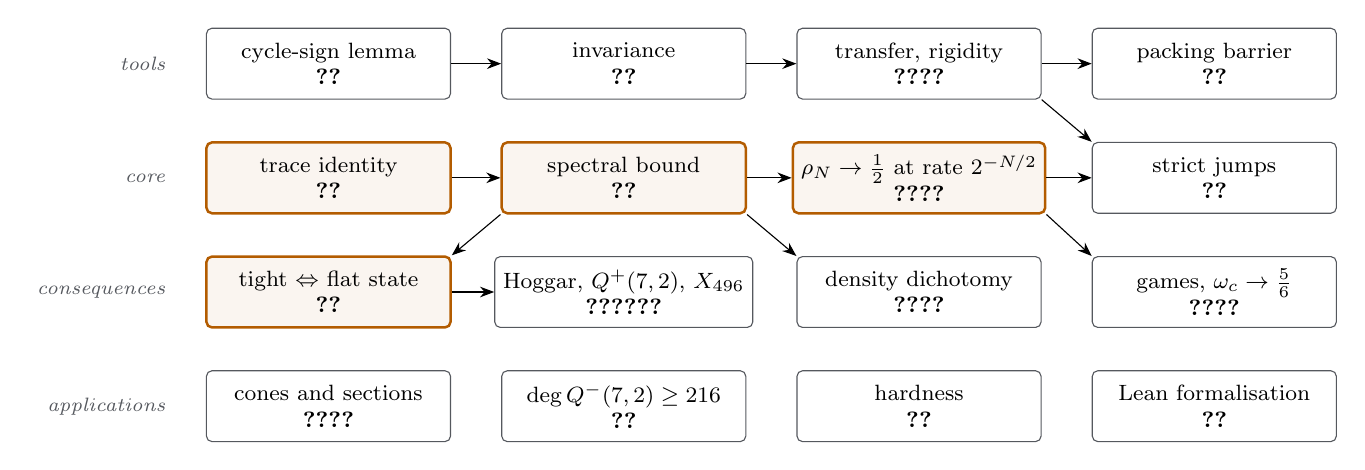
\begin{tikzpicture}[every node/.style={font=\footnotesize},>={Stealth[length=1.8mm]},
  box/.style={draw=inkgray,rounded corners=2pt,align=center,inner sep=3pt,minimum width=31mm,minimum height=9mm,fill=white},
  hot/.style={box,draw=numorange,line width=0.9pt,fill=numorange!6},
  row/.style={font=\scriptsize\itshape,text=inkgray,anchor=east}]
\def\dx{3.75}\def\dy{1.45}
% row 1: foundations
\node[box] (cyc) at (0,0) {cycle-sign lemma\\\cref{lem:cyclesign}};
\node[box] (inv) at (\dx,0) {invariance\\\cref{cor:invariance}};
\node[box] (tr)  at (2*\dx,0) {transfer, rigidity\\\cref{thm:transfer,thm:rigidity}};
\node[box] (pack) at (3*\dx,0) {packing barrier\\\cref{cor:barrier}};
% row 2: spectral core
\node[hot] (trace) at (0,-\dy) {trace identity\\\cref{thm:trace}};
\node[hot] (spec) at (\dx,-\dy) {spectral bound\\\cref{thm:spectral}};
\node[hot] (lim) at (2*\dx,-\dy) {$\rho_N\to\frac12$ at rate $2^{-N/2}$\\\cref{thm:limit,thm:rate}};
\node[box] (jump) at (3*\dx,-\dy) {strict jumps\\\cref{thm:jumps}};
% row 3: consequences
\node[hot] (tight) at (0,-2*\dy) {tight $\Leftrightarrow$ flat state\\\cref{thm:tight}};
\node[box] (hog) at (\dx,-2*\dy) {Hoggar, $\Qp7$, $X_{496}$\\\cref{thm:hoggar,thm:qp7,thm:x496}};
\node[box] (dens) at (2*\dx,-2*\dy) {density dichotomy\\\cref{thm:den1,thm:den3}};
\node[box] (game) at (3*\dx,-2*\dy) {games, $\omega_c\to\frac56$\\\cref{thm:game,thm:gameW}};
% row 4: geometry and complexity
\node[box] (sec) at (0,-3*\dy) {cones and sections\\\cref{thm:cone,thm:Wsections}};
\node[box] (qm7) at (\dx,-3*\dy) {$\deg\Qm7\ge216$\\\cref{thm:216}};
\node[box] (hard) at (2*\dx,-3*\dy) {hardness\\\cref{thm:induced}};
\node[box] (lean) at (3*\dx,-3*\dy) {Lean formalisation\\\cref{sec:lean}};
\draw[->] (cyc)--(inv); \draw[->] (inv)--(tr); \draw[->] (tr)--(pack);
\draw[->] (trace)--(spec); \draw[->] (spec)--(lim); \draw[->] (lim)--(jump);
\draw[->] (tr.south east)--(jump.north west);
\draw[->] (spec.south west)--(tight.north east);
\draw[->] (tight)--(hog);
\draw[->] (spec.south east)--(dens.north west);
\draw[->] (lim.south east)--(game.north west);
\node[row] at (-1.95,0) {tools};
\node[row] at (-1.95,-\dy) {core};
\node[row] at (-1.95,-2*\dy) {consequences};
\node[row] at (-1.95,-3*\dy) {applications};
\end{tikzpicture}
\caption{How the results depend on each other. The orange boxes are the spectral core of the paper. The bottom
row uses the tools of the top row (invariance, transfer and the cycle-sign lemma) and, for $\Qm7$, the
spectral bound only as a point of comparison.}
\label{fig:roadmap}
\end{figure}

%% ---- sec-prelim.tex ----
\section{Preliminaries}\label{sec:prelim}
%=====================================================================================================

\subsection{Pauli observables and lines}
We write an $N$-qubit Pauli operator, up to phase, as a vector $p=(x\,|\,z)\in\F^{2N}$, and use the
Hermitian representative
\[
  P_p=P(p)=i^{\,x\cdot z}\,X^{x}Z^{z},\qquad X^x=\textstyle\bigotimes_k X^{x_k},\; Z^z=\bigotimes_k Z^{z_k},
\]
where $x\cdot z\in\Z$ is the integer dot product, i.e.\ the number $y(p)$ of $Y$ factors. Concretely, in the
computational basis indexed by $c\in\F^N$,
\begin{equation}\label{eq:paulimatrix}
  P_p\,\ket{c}\;=\;i^{\,y(p)+2\,z\cdot c}\,\ket{c+x}.
\end{equation}
This is the definition used in the formalisation, where $P_p$ is an explicit $2^N\times2^N$ complex matrix.
We write $d=2^N$, $V=\F^{2N}$ and $\Vs=V\setminus\{0\}$. The symplectic form
$\omega(p,q)=x\cdot z'+z\cdot x' \bmod 2$ records commutation.

\begin{lemma}[Pauli algebra]\label{lem:pauli}
For all $p,q\in V$:
\begin{enumerate}[label=(\roman*)]
\item $P_pP_q=i^{\beta(p,q)}P_{p+q}$ with $\beta(p,q)=y(p)+y(q)+2\,z_p\cdot x_q-y(p+q)\in\Z/4$;
\item $P_pP_q=(-1)^{\omega(p,q)}P_qP_p$, \ $P_p^2=I$, \ $P_p^\dagger=P_p$;
\item $\tr P_p=d\,[p=0]$ and $\tr(P_pP_q)=d\,[p=q]$;
\item (completeness) for every vector $v\in\C^d$, $\sum_{p\in V}\bra{v}P_p\ket{v}^2=d\,\|v\|^4$, and
$\sum_{p\in V}\bra{v}P_p\ket{v}\,P_p=d\,\proj{v}$.
\end{enumerate}
\lean{pauli\_mul, pauli\_comm, trace\_pauli\_mul, pauli\_completeness, pauli\_expand}
\end{lemma}
\begin{proof}
(i) and (ii) are direct computations from~\eqref{eq:paulimatrix}: $P_pP_q\ket c=i^{y(q)+2z_q\cdot c}\,
i^{y(p)+2z_p\cdot(c+x_q)}\ket{c+x_p+x_q}$, and comparing with $P_{p+q}\ket c$ gives (i), with
$\beta(p,q)-\beta(q,p)=2\omega(p,q)$ for (ii). $P_p^2=I$ follows from (i) with $q=p$, since
$2y(p)+2z_p\cdot x_p=4y(p)\equiv0$; as $P_p$ is a permutation matrix times a diagonal unitary, it is unitary, so
$P_p^\dagger=P_p^{-1}=P_p$. (iii) The diagonal of $P_p$ vanishes unless $x=0$, and for $x=0$ the trace is
$\sum_c(-1)^{z\cdot c}=d[z=0]$; then use (i). (iv) The $d^2$ matrices $P_p$ are orthogonal for the trace inner
product by (iii), hence a basis of $M_d(\C)$, and $\proj v=d^{-1}\sum_p\tr(P_p\proj v)P_p$. Taking
$\tr(\,\cdot\,\proj v)$ gives the first identity.
\end{proof}

The Pauli group law used in the formalisation is the abstract version of (i): on pairs $(k,p)\in\Z/4\times V$,
$(k_1,p)(k_2,q)=(k_1+k_2+2\,z_p\cdot x_q,\ p+q)$, with canonical elements $(y(p),p)$. It is associative, $(k,0)$ is
central, and $(0,p)(0,q)=(2\omega(p,q),0)\,(0,q)(0,p)$ \leanin{mulPG\_assoc, mulPG\_central, comm\_rule, canon\_sq}.

\begin{definition}
A \emph{line} is a set $\{a,b,c\}$ of three distinct points with $a+b+c=0$ and $\omega(a,b)=0$ (hence all three
pairwise commute). Its \emph{sign} $e\in\F$ is defined by $P_aP_bP_c=(-1)^{e}I$; the product is $\pm I$ because
the three operators commute and their labels sum to zero, and it does not depend on the order
\leanin{signK\_even, sign\_symm}. We also write $\chi(\ell)=(-1)^{e(\ell)}$; equivalently $P_aP_b=\chi(\ell)P_c$
for any two points $a,b$ of $\ell$.
\end{definition}

The lines of $V$ are the lines of the symplectic polar space $\W{2N-1}$. A \emph{quadratic form} $q$ on
$V$ polarising to $\omega$, i.e.\ with $q(a+b)=q(a)+q(b)+\omega(a,b)$, defines a quadric; its points are the
non-zero $p$ with $q(p)=0$ and its lines are the lines all of whose points lie on it. We use the hyperbolic form
$q^+(x|z)=x\cdot z \bmod 2$, whose points are exactly the Pauli operators with an even number of $Y$ factors,
i.e.\ the real symmetric Pauli observables, and the elliptic form $q^-(x|z)=x\cdot z+x_1+z_1\bmod 2$. We write
$\Qp{2N-1}$, $\Qm{2N-1}$ for these configurations. \Cref{tab:counts} lists their sizes.

\begin{table}[h]
\centering\small
\begin{tabular}{@{}lcccccc@{}}
\toprule
$N$ & $\W{2N-1}$ & & $\Qp{2N-1}$ & & $\Qm{2N-1}$ &\\
& points & lines & points & lines & points & lines\\\midrule
2 & 15 & 15 & 9 & 6 & 5 & 0\\
3 & 63 & 315 & 35 & 105 & 27 & 45\\
4 & 255 & 5355 & 135 & 1575 & 119 & 1071\\
5 & 1023 & 86955 & 527 & 23715 & 495 & 19635\\\bottomrule
\end{tabular}
\caption{Points and lines of the geometries used in this paper. In general $\W{2N-1}$ has $4^N-1$ points and
$(4^N-1)(4^N-4)/12$ lines \leanin{lines\_W}.}
\label{tab:counts}
\end{table}

\subsection{Configurations and the contextuality degree}
\begin{definition}
A \emph{configuration} $C$ on $n$ qubits is a finite set $\Lines(C)$ of lines; its points $\Pts(C)$ are those
lying on its lines, and each line carries its sign $e_C(\ell)$. A \emph{value assignment} is a map
$s:\Pts(C)\to\F$ (value $(-1)^{s(p)}$). A line $\ell=\{a,b,c\}$ is \emph{violated} by $s$ if
$s(a)+s(b)+s(c)\neq e_C(\ell)$. The \emph{degree} $\deg(C)$ is the minimum number of violated lines over all
assignments, and the \emph{contextuality ratio} is $\rho(C)=\deg(C)/|\Lines(C)|$.
\end{definition}

\begin{definition}[induced configuration]
For a finite set $X\subseteq\Vs$, the \emph{induced configuration} $C(X)$ has point set $X$ and \emph{all} lines
$\{a,b,a+b\}\subseteq X$ with $\omega(a,b)=0$. We write $\Lines_X$ for its lines and $\deg X$ for its degree.
$\W{2N-1}$ is induced by $\Vs$; quadrics and subspace sections are induced as well, because
$q(a+b)=q(a)+q(b)+\omega(a,b)$.
\end{definition}

Most of the spectral part of the paper is about induced configurations; transfer, cycles and hardness also apply
to arbitrary ones.

Let $H\in\F^{\Lines\times\Pts}$ be the incidence matrix of $C$. Then the set of violated lines of $s$ has
indicator $Hs+e_C$, so
\begin{equation}\label{eq:coset}
  \deg(C)=\min_{s\in\F^{\Pts}}|Hs+e_C|=d\bigl(e_C,\ \im H\bigr),
\end{equation}
the Hamming distance from $e_C$ to the binary code $\im H$. In particular $\deg(C)$ depends only on the coset
$e_C+\im H$. Since $(\im H)^\perp=\ker H^{\mathsf T}$, the coset is determined by the linear functional
$y\mapsto y\cdot e_C$ on the \emph{cycle space} $\ker H^{\mathsf T}$, whose elements are the sets of lines covering
every point an even number of times. A cycle $y$ with $y\cdot e_C=1$ is an \emph{odd cycle}; $C$ is contextual
($\deg(C)>0$) iff it has one. Since a uniformly random assignment violates each line with probability $1/2$,
\begin{equation}\label{eq:half}
\deg(C)\le|\Lines(C)|/2\qquad\text{for every configuration}
\end{equation}
\leanin{Config.deg\_le\_half}. The degree depends only on the coset $e_C+\im H$ \leanin{Config.deg\_gauge}, and two
sign vectors with the same parity on every cycle define the same coset
\leanin{Config.deg\_eq\_of\_cycles}.

\subsection{Operational meaning}
For a line $\ell=\{a,b,c\}$ the three observables are jointly measurable, and the product of their outcomes is the
outcome of $P(a)P(b)P(c)=(-1)^{e(\ell)}I$. Write $\langle abc\rangle$ for the expectation of the product of the
three outcomes and set
\begin{equation}\label{eq:witness}
\beta_C=\sum_{\ell\in\Lines(C)}(-1)^{e(\ell)}\langle abc\rangle_\ell .
\end{equation}
\begin{proposition}[noncontextuality inequality]\label{prop:operational}
Let $C$ have $m$ lines.
\begin{enumerate}[label=(\roman*)]
\item Every noncontextual hidden-variable model (deterministic, context-independent outcome assignments and their
probabilistic mixtures) satisfies $\beta_C\le m-2\deg(C)$, and the bound is attained.
\item Quantum mechanics gives $\beta_C=m$ in every state.
\item If every signed correlator is attenuated by a common factor $v\in[0,1]$ (data $v\cdot1$ per line), the
inequality is violated if and only if $v>1-2\deg(C)/m$.
\end{enumerate}
\lean{Config.nc\_bound, attenuation\_iff}
\end{proposition}
\begin{proof}
(i) A deterministic assignment contributes $+1$ for every satisfied and $-1$ for every violated line, hence
$m-2|V|\le m-2\deg(C)$, with equality for an optimal assignment; mixtures are convex combinations.
(ii) For each line the signed product of outcomes is the eigenvalue of $(-1)^{e(\ell)}P(a)P(b)P(c)=I$.
(iii) The attenuated value is $vm$.
\end{proof}
Thus the degree is exactly half the state-independent quantum--classical gap of the parity test~\eqref{eq:witness}.
Statement (iii) concerns this idealised symmetric noise model only. An actual experiment must also address
imperfect compatibility, measurement disturbance and finite statistics; see~\cite{Budroni2022} for these
issues. We make no claim about experimental thresholds beyond (iii).

\begin{remark}[frustration]\label{rem:frustration}
With spins $\sigma_p=(-1)^{s(p)}$, the number of violated lines is the energy of the three-spin Ising Hamiltonian
$\mathcal H_C=\sum_{\ell}\frac12\bigl(1-(-1)^{e(\ell)}\sigma_a\sigma_b\sigma_c\bigr)$. The degree is its
ground-state energy. Translating $e_C$ by $\im H$ is a gauge transformation, and odd cycles are frustrated loops in
the sense of Toulouse~\cite{Toulouse1977}. Contextuality degree is therefore, precisely, the minimal frustration
of a gauge class of signed three-body constraints; Pauli geometry restricts which gauge classes occur
(\cref{lem:cyclesign}).
\end{remark}

\subsection{Signs of cycles depend only on commutation}
\begin{lemma}[cycle-sign lemma]\label{lem:cyclesign}
Let $y=\{\ell_1,\dots,\ell_k\}$ be a cycle of $C$. Write the points of $\ell_1$, then those of $\ell_2$, and so on,
as a word $w=w_1w_2\cdots w_{3k}$ in the points of $C$, and fix any total order $\prec$ on $\Pts(C)$. Then
\[
  \sum_{j=1}^{k} e_C(\ell_j)\;=\;\sum_{\substack{1\le r<t\le 3k\\ w_t\prec w_r}}\omega(w_r,w_t)\pmod 2 .
\]
In particular the parity of a cycle is a function of the incidence structure and of the restriction of $\omega$
to $\Pts(C)$ only.
\lean{cycle\_parity\_eq\_inversions}
\end{lemma}
\begin{proof}
Evaluate $M=P(w_1)P(w_2)\cdots P(w_{3k})$ in two ways. Grouping the factors line by line,
$M=\prod_j (-1)^{e_C(\ell_j)}I$. Alternatively, sort the word into $\prec$-increasing order by adjacent
transpositions; each transposition of $P(p)P(q)$ contributes $(-1)^{\omega(p,q)}$, and every pair of positions
$r<t$ with $w_t\prec w_r$ is transposed exactly once (bubble sort performs exactly the inversions). The sorted
word is $\prod_p P(p)^{m_p}$ with every multiplicity $m_p$ even, because $y$ is a cycle, so it equals $I$.
Comparing the two expressions gives the claim.
\end{proof}

\begin{corollary}[invariance of the degree]\label{cor:invariance}
Let $C,C'$ be configurations, possibly on different numbers of qubits, and $\pi:\Pts(C)\to\Pts(C')$ a bijection
that maps lines of $C$ onto lines of $C'$ and satisfies $\omega(\pi p,\pi q)=\omega(p,q)$. Then
$\deg(C)=\deg(C')$, and $\pi$ maps optimal assignments to optimal assignments (as $s\mapsto s\circ\pi^{-1}$,
after adding a fixed element of the code).
\lean{deg\_invariant}
\end{corollary}
\begin{proof}
Identify incidence matrices through $\pi$. By Lemma~\ref{lem:cyclesign} (with the order on $\Pts(C')$ transported
by $\pi$) every cycle has the same parity in both, so $e_{C'}\circ\pi-e_C\in(\ker H^{\mathsf T})^\perp=\im H$.
By~\eqref{eq:coset} the degrees coincide; the second statement follows by translating $s$ by a preimage of
$e_{C'}\circ\pi-e_C$.
\end{proof}

Corollary~\ref{cor:invariance} recovers the hypergram invariance of~\cite{MullerGiorgetti2025}. We use three
instances: (i) every $g\in\Sp(2N,2)$ preserves $\omega$ and maps lines to lines (it is induced by a Clifford
unitary, but we do not need this); (ii) the padding $p\mapsto(p\,|\,0)$ into more qubits; (iii) a linear
isometry from a non-degenerate subspace onto $\F^{2m}$. For induced configurations the hypotheses can be weakened,
which matters for sections (\cref{sec:geometry}).

\begin{corollary}[maps between induced configurations]\label{cor:inducedmap}
Let $X\subseteq\Vs(N)$ and $\theta:X\to\Vs(N')$ be injective, with $\omega(\theta a,\theta b)=\omega(a,b)$ for
$a,b\in X$, and additive on lines: if $a,b,a+b\in X$ with $\omega(a,b)=0$ then $\theta(a+b)=\theta a+\theta b$, and
conversely $\theta c=\theta a+\theta b$ forces $c=a+b$. Then $\theta$ is a bijection $\Lines_X\to\Lines_{\theta X}$
and $\deg\theta(X)=\deg X$. This holds in particular for linear maps that preserve $\omega$ on $X$ and are injective
on $\operatorname{span}X$. \lean{deg\_configX\_fun, deg\_configX\_map}
\end{corollary}
\begin{proof}
The hypotheses say exactly that $\theta$ maps lines onto lines and induces a bijection between them; apply
\cref{cor:invariance}. For a linear map injective on the span, $\theta c=\theta a+\theta b=\theta(a+b)$ forces
$c=a+b$.
\end{proof}


%% ---- sec-transfer.tex ----
\section{Symmetry: transfer, rigidity and local certificates}\label{sec:transfer}
%=====================================================================================================

\begin{definition}
Let $G$ be a configuration on $N$ qubits. Its \emph{symmetry group} is
$\operatorname{Aut}(G)=\{g\in\Sp(2N,2): g(\Lines(G))=\Lines(G)\}$. An \emph{embedding} of a configuration $S$
into $G$ is an injective map $\pi:\Pts(S)\to\Pts(G)$ with $\omega(\pi p,\pi q)=\omega(p,q)$ that maps every line
of $S$ onto a line of $G$. We write $\pi(S)$ for the sub-configuration of $G$ formed by the image lines, with the
signs it inherits from $G$.
\end{definition}

By Corollary~\ref{cor:invariance}, $\deg\pi(S)=\deg S$ for every embedding; the inherited signs of $\pi(S)$ need
not agree with those of $S$ line by line, but they lie in the same coset. Embeddings need not be linear, and $S$ may
live on a different number of qubits.

The basic counting step does not need a group at all.

\begin{lemma}[uniform cover]\label{lem:cover}
Let $C$ be a configuration and $S_1,\dots,S_r$ sub-configurations of $C$ (sets of lines of $C$ with the inherited
signs) such that every line of $C$ lies in at most $c$ of them. Then for every assignment with violated set $V$,
\[
  c\,|V|\ \ge\ \sum_{i=1}^r|V\cap\Lines(S_i)|\ \ge\ \sum_{i=1}^r\deg S_i ,\qquad\text{hence}\qquad
  \deg C\ \ge\ \Bigl\lceil\frac1c\sum_i\deg S_i\Bigr\rceil .
\]
If every line lies in exactly $c$ of the $S_i$ and $\deg C=\frac1c\sum_i\deg S_i$, then every optimal assignment
of $C$ is optimal on every $S_i$.
\lean{Config.uniform\_cover\_deg, uniform\_cover\_rigid}
\end{lemma}
\begin{proof}
Count pairs $(\ell,i)$ with $\ell\in V\cap\Lines(S_i)$ in two ways. The restriction of an assignment of $C$ to
$S_i$ is an assignment of $S_i$, so it violates at least $\deg S_i$ of its lines. In the equality case all the
inequalities are equalities.
\end{proof}

\begin{theorem}[transfer]\label{thm:transfer}
Let $\Gamma\le\operatorname{Aut}(G)$ act transitively on $\Lines(G)$, and let $S$ embed into $G$. Then
\[
  \rho(G)\ \ge\ \rho(S),\qquad\text{and in fact}\qquad
  \deg G\ \ge\ \Bigl\lceil \frac{|\Lines(G)|\,\deg S}{|\Lines(S)|}\Bigr\rceil .
\]
\lean{Config.transfer, transfer\_cover}
\end{theorem}
\begin{proof}
Let $s$ be an optimal assignment of $G$ and $V$ its set of violated lines, $|V|=\deg G$. For $g\in\Gamma$, the
map $g\circ\pi$ is again an embedding, so the restriction of $s$ to $g\pi(S)$ violates at least
$\deg g\pi(S)=\deg S$ of its lines; these are exactly the lines of $V\cap\Lines(g\pi(S))$. Summing over $\Gamma$
and exchanging the order of summation,
\[
|\Gamma|\,\deg S\ \le\ \sum_{g\in\Gamma}\bigl|V\cap g\,\pi(\Lines(S))\bigr|
=\sum_{\ell\in V}\ \sum_{m\in\pi(\Lines(S))}\bigl|\{g\in\Gamma:gm=\ell\}\bigr|
=|V|\,|\Lines(S)|\,\frac{|\Gamma|}{|\Lines(G)|},
\]
where we used that $\pi$ is injective on lines and that, by transitivity, $|\{g:gm=\ell\}|=|\Gamma_m|
=|\Gamma|/|\Lines(G)|$ for all lines $m,\ell$ of $G$. Dividing
gives $|V|\ge\deg S\,|\Lines(G)|/|\Lines(S)|$, and $|V|$ is an integer.
\end{proof}

\begin{theorem}[equality and rigidity]\label{thm:rigidity}
In the setting of Theorem~\ref{thm:transfer}, call an assignment $s$ of $G$ \emph{$S$-tight} if it violates
exactly $\deg S$ lines of $g\pi(S)$ for every $g\in\Gamma$. The following are equivalent:
\begin{enumerate}[label=(\alph*)]
\item $\rho(G)=\rho(S)$;
\item every optimal assignment of $G$ is $S$-tight;
\item some assignment of $G$ is $S$-tight.
\end{enumerate}
Every $S$-tight assignment is optimal. In particular, if $|\Lines(G)|\deg S/|\Lines(S)|\notin\mathbb Z$ then
$\rho(G)>\rho(S)$ and no assignment of $G$ is $S$-tight.
\lean{Config.transfer\_rigid}
\end{theorem}
\begin{proof}
(a)$\Rightarrow$(b): for optimal $s$ the displayed chain in the proof of Theorem~\ref{thm:transfer} is an
equality, and each of its $|\Gamma|$ terms is at least $\deg S$, so each equals $\deg S$.
(b)$\Rightarrow$(c) is trivial. (c)$\Rightarrow$(a): for an $S$-tight $s$ the same double count gives
$|V|=\rho(S)|\Lines(G)|$, so $\deg G\le\rho(S)|\Lines(G)|\le\deg G$; this also shows that $s$ is optimal.
The last statement follows because $\deg G$ is an integer.
\end{proof}

For $G=\Qp{7}$ and $S$ a doily, where $\rho(G)=\rho(S)=\frac15$~\cite{LiGuptaGanesh2026},
Theorem~\ref{thm:rigidity} yields that every optimal assignment of $\Qp7$ violates exactly three lines of every
doily, the local structure exploited in~\cite{LiGuptaGanesh2026}. The last statement of the theorem is the
integrality phenomenon exploited in \cref{sec:qm7}.

\subsection{Stability}
Rigidity concerns exact equality. The double count behind Theorem~\ref{thm:transfer} is in fact an identity, which
also controls assignments that are only close to optimal.

\begin{lemma}[local--global identity]\label{lem:localglobal}
In the setting of Theorem~\ref{thm:transfer}, for every assignment of $G$ with violated set $V$,
\[
\frac1{|\Gamma|}\sum_{g\in\Gamma}\bigl|V\cap g\pi(\Lines(S))\bigr|=\frac{|\Lines(S)|}{|\Lines(G)|}\,|V| .
\]
\end{lemma}
\begin{proof}
This is the computation in the proof of Theorem~\ref{thm:transfer}, which uses only transitivity and not optimality.
\end{proof}

\begin{theorem}[stability]\label{thm:stability}
In the setting of Theorem~\ref{thm:transfer}, let $s$ be any assignment of $G$ with violated set $V$, write
$\Delta_g=|V\cap g\pi(\Lines(S))|-\deg S\ge0$ for the \emph{local excess} of the translate $g\pi(S)$, and
$D=|V|-\rho(S)|\Lines(G)|$ for the \emph{global excess}. Then
\[
\frac1{|\Gamma|}\sum_{g\in\Gamma}\Delta_g=\frac{|\Lines(S)|}{|\Lines(G)|}\,D,
\]
and the fraction $\tau$ of non-tight translates ($\Delta_g>0$) satisfies
\[
\frac{|\Lines(S)|}{|\Lines(G)|}\cdot\frac{D}{|\Lines(S)|-\deg S}\ \le\ \tau\ \le\ \frac{|\Lines(S)|}{|\Lines(G)|}\,D .
\]
\lean{Config.uniform\_cover\_excess}
\end{theorem}
\begin{proof}
The identity is Lemma~\ref{lem:localglobal} minus $\deg S$. For the bounds, $1\le\Delta_g\le|\Lines(S)|-\deg S$
whenever $\Delta_g>0$, so $\tau|\Gamma|\le\sum_g\Delta_g\le\tau|\Gamma|(|\Lines(S)|-\deg S)$.
\end{proof}

\begin{corollary}\label{cor:stability}
\begin{enumerate}[label=(\roman*)]
\item (near-optimal assignments) If $|V|\le\deg G+t$, then at most a fraction
$\frac{|\Lines(S)|}{|\Lines(G)|}(\deg G-\rho(S)|\Lines(G)|+t)$ of the translates are non-tight. In particular,
when $\rho(G)=\rho(S)$, an assignment within $t$ of optimal is tight on all but a fraction
$t\,|\Lines(S)|/|\Lines(G)|$ of the translates.
\item (forced non-tightness) Every assignment of $G$, optimal or not, is non-tight on at least a fraction
$\frac{|\Lines(S)|\,(\lceil\rho(S)|\Lines(G)|\rceil-\rho(S)|\Lines(G)|)}{|\Lines(G)|\,(|\Lines(S)|-\deg S)}$ of the
translates.
\end{enumerate}
\end{corollary}
\begin{proof}
(i) Use the upper bound on $\tau$ with $D\le\deg G+t-\rho(S)|\Lines(G)|$. (ii) Use the lower bound with
$D\ge\lceil\rho(S)|\Lines(G)|\rceil-\rho(S)|\Lines(G)|$, which holds because $|V|$ is an integer
$\ge\deg G\ge\lceil\rho(S)|\Lines(G)|\rceil$.
\end{proof}

For example, in $\Qm7$ with doilies, every assignment has average doily excess at least $15\cdot0.8/1071>0.011$;
and if $\deg\Qm7=315$ (\cref{conj:517}), every optimal assignment violates on average
$315\cdot15/1071\approx4.41$ lines per doily, so at least $11.7\%$ of the doilies are non-tight.

\subsection{Several orbits: the profile bound}\label{sec:profile}
Line-transitivity is a strong hypothesis. In general the lines of $G$ split into $\Gamma$-orbits, and several
witnesses can be combined.

\begin{theorem}[profile bound]\label{thm:profile}
Let $\Gamma\le\operatorname{Aut}(G)$ have line orbits $O_1,\dots,O_r$, and let $S_1,\dots,S_k$ be configurations with
embeddings $\pi_j$ into $G$. Put $d_j=\deg S_j$ and $a_{ij}=|\pi_j(\Lines(S_j))\cap O_i|$. For every assignment of
$G$, its \emph{violation profile} $n_i=|V\cap O_i|$ satisfies
\begin{equation}\label{eq:profile}
\sum_{i=1}^r\frac{a_{ij}}{|O_i|}\,n_i\ \ge\ d_j\qquad(j=1,\dots,k).
\end{equation}
Consequently $\deg G\ge\mathrm{IP}:=\min\{\sum_in_i:\ n\in\mathbb Z^r,\ 0\le n_i\le|O_i|,\ \eqref{eq:profile}\}$,
and $\mathrm{IP}$ is at least the value of the linear relaxation, which by LP duality equals
\[
\mathrm{LP}=\max\Bigl\{\sum_jW_jd_j:\ W\ge0,\ \sum_ja_{ij}W_j\le|O_i|\ (i=1,\dots,r)\Bigr\}.
\]
\lean{Config.profile\_bound}
\end{theorem}
\begin{proof}
Fix $j$. For lines $m,\ell$ in the same orbit $O_i$, $|\{\gamma\in\Gamma:\gamma m=\ell\}|=|\Gamma|/|O_i|$. Hence
\[
\frac1{|\Gamma|}\sum_{\gamma\in\Gamma}\bigl|V\cap\gamma\pi_j(\Lines(S_j))\bigr|
=\sum_{m\in\pi_j(\Lines(S_j))}\frac{|V\cap O_{i(m)}|}{|O_{i(m)}|}=\sum_i\frac{a_{ij}}{|O_i|}n_i ,
\]
and the left-hand side is at least $d_j$ by Corollary~\ref{cor:invariance}, as each $\gamma\pi_j$ is an embedding.
The remaining statements are immediate, with the dual LP in the variables $y_i=n_i/|O_i|$.
\end{proof}

For $r=1$ the integer program returns $\lceil\rho(S)|\Lines(G)|\rceil$, i.e.\ Theorem~\ref{thm:transfer}. The LP
side is the $\Gamma$-symmetric version of the packings of Section~\ref{sec:dual}. Complementary slackness gives a
multi-orbit form of rigidity.

\begin{corollary}[multi-orbit rigidity]\label{cor:mrigid}
If $\deg G=\mathrm{LP}$ and $W^*$ is an optimal solution of the LP, then every optimal assignment of $G$ is tight on
every $\Gamma$-translate of $\pi_j(S_j)$ for each $j$ with $W^*_j>0$.
\end{corollary}
\begin{proof}
Let $n$ be the profile of an optimal assignment and $A_j=\sum_ia_{ij}n_i/|O_i|$ the average in the proof above. Since
$\sum_ja_{ij}W^*_j\le|O_i|$ and $n_i\ge0$,
$\deg G=\sum_in_i\ge\sum_in_i\sum_ja_{ij}W^*_j/|O_i|=\sum_jW^*_jA_j\ge\sum_jW^*_jd_j=\mathrm{LP}=\deg G$.
Hence $A_j=d_j$ whenever $W^*_j>0$, and since every translate violates at least $d_j$ lines, all are tight.
\end{proof}

Section~\ref{sec:cones} gives an application in which $G$ is not line-transitive, so Theorem~\ref{thm:transfer}
does not apply, but Theorem~\ref{thm:profile} with two orbits determines the degree exactly.

\subsection{Extremality of the symplectic polar space}
We use Witt's theorem~\cite{Taylor1992}: $\Sp(2N,2)$ acts transitively on the lines of $\W{2N-1}$, and the
orthogonal group $\Orth(q)\le\Sp(2N,2)$ of a non-degenerate quadratic form $q$ acts transitively on the lines of
its quadric. Over $\F$, non-degenerate quadratic forms on $\F^{2N}$ are classified by their Arf invariant
(hyperbolic $=0$, elliptic $=1$), which is additive under orthogonal sums. The formalisation avoids Witt's theorem
for the symplectic case: line-transitivity of $\Sp(2N,2)$ is proved there with explicit products of transvections
$x\mapsto x+\omega(x,c)c$ \leanin{Sp\_trans\_lines}

\begin{corollary}[extremality of the full space]\label{cor:extremal}
For $N\ge2$ let $\rho_N=\rho(\W{2N-1})$.
\begin{enumerate}[label=(\roman*)]
\item $\rho(S)\le\rho_N$ for every configuration $S$ on at most $N$ qubits, with equality iff every optimal
assignment of $\W{2N-1}$ is $S$-tight.
\item $\rho_N$ is non-decreasing in $N$, and $\frac15\le\rho_N\le\frac12$ for $N\ge2$.
\item $\rho(\Qp{2N-1})\le\rho_N$ and $\rho(\Qm{2N-1})\le\rho_N$.
\item $\rho(Q^{\varepsilon}(2N+1,2))\ge\max\{\rho(\Qp{2N-1}),\rho(\Qm{2N-1})\}$ for $\varepsilon\in\{+,-\}$.
\end{enumerate}
\lean{rho\_max, rho\_mono}
\end{corollary}
\begin{proof}
(i) Pad $S$ with identity factors and include it in $\W{2N-1}$; apply Theorems~\ref{thm:transfer}
and~\ref{thm:rigidity} with $\Gamma=\Sp(2N,2)$. (ii) Monotonicity is (i) applied to $S=\W{2N-1}$ padded into $N+1$
qubits. The lower bound is $\rho_2=\frac15$ (\cref{prop:doily}) and monotonicity; the upper bound holds
for every configuration. (iii) Quadric lines are lines of $\W{2N-1}$; apply (i). (iv) Let $q$ be a form of type
$\varepsilon$ on $\F^{2N+2}$ and $\delta\in\{+,-\}$. Choose a non-degenerate plane $E$ on which $q$ has type
$\varepsilon\delta$ (with $+\cdot+=-\cdot-=+$); then $q|_{E^\perp}$ has type $\delta$ by additivity of the Arf
invariant, and a linear isometry $E^\perp\to(\F^{2N},q^{\delta})$ maps the points and lines of $q$ inside
$E^\perp$ bijectively onto those of $Q^\delta(2N-1,2)$, preserving $\omega$. This is an embedding of
$Q^\delta(2N-1,2)$ into $Q^\varepsilon(2N+1,2)$; apply Theorem~\ref{thm:transfer} with $\Gamma=\Orth(q)$.
\end{proof}

So among all $N$-qubit configurations the full space $\W{2N-1}$ is the most contextual per context, and
\cref{thm:rigidity} says exactly which sub-configurations share its ratio. The next three sections compute
$\rho_N$ asymptotically.

\subsection{Local certificates and their limits}\label{sec:dual}
%=====================================================================================================

Lower bounds on the degree come from certificates that every assignment must violate. The most basic certificate is
an odd cycle: if $H^{\mathsf T}y=0$ and $y\cdot e_C=1$, then for every assignment $s$,
$y\cdot(Hs+e_C)=1$, so every assignment violates an odd number, hence at least one, of the lines of $y$. More
generally, any sub-configuration $S\subseteq C$ (with inherited signs) forces at least $\deg S$ violations among
its own lines.

\begin{definition}
Let $\mathcal S$ be a family of sub-configurations of $C$. A \emph{packing} is a weighting $w:\mathcal S\to
\mathbb R_{\ge0}$ with $\sum_{S\ni\ell}w_S\le1$ for every line $\ell$ of $C$; its \emph{value} is
$\sum_S w_S\deg S$. Let $\nu_{\mathcal S}(C)$ be the supremum of the values.
\end{definition}
Odd-cycle packings are the special case in which $\mathcal S$ consists of odd cycles, each of degree at least one.

\begin{theorem}[local certificates]\label{thm:packing}
For every configuration $C$ and family $\mathcal S$ of sub-configurations:
\begin{enumerate}[label=(\alph*)]
\item $\deg C\ge\nu_{\mathcal S}(C)$;
\item $\nu_{\mathcal S}(C)\le|\Lines(C)|\cdot\sup_{S\in\mathcal S}\rho(S)$;
\item if some $\Gamma\le\operatorname{Aut}(C)$ is transitive on $\Lines(C)$ and $\mathcal S$ is $\Gamma$-invariant, then
$\nu_{\mathcal S}(C)=|\Lines(C)|\cdot\max_{S\in\mathcal S}\rho(S)$.
\end{enumerate}
\lean{packing\_le\_deg, packing\_le\_ratio, packing\_orbit}
\end{theorem}
\begin{proof}
(a) For an optimal assignment with violated set $V$,
$\sum_Sw_S\deg S\le\sum_Sw_S|V\cap S|=\sum_{\ell\in V}\sum_{S\ni\ell}w_S\le|V|$.
(b) $\sum_Sw_S\deg S\le r\sum_Sw_S|\Lines(S)|=r\sum_\ell\sum_{S\ni\ell}w_S\le r|\Lines(C)|$ with
$r=\sup\rho(S)$.
(c) Let $S$ attain the maximum and let $O$ be its $\Gamma$-orbit. By transitivity every line of $C$ lies in the same
number $|O|\,|\Lines(S)|/|\Lines(C)|$ of members of $O$. The uniform weight
$w=|\Lines(C)|/(|O|\,|\Lines(S)|)$ on $O$ is therefore a packing of value $|\Lines(C)|\rho(S)$; combine with (b).
\end{proof}

Theorem~\ref{thm:packing}(c) says that in symmetric geometries the transfer bound is the best lower bound obtainable
by \emph{any} fractional combination of local witnesses from a given invariant family. Only integrality can add to
it, as in Theorem~\ref{thm:rigidity}. Combined with the three-qubit bound this gives a barrier.

\begin{corollary}[three-qubit barrier]\label{cor:barrier}
Call a configuration \emph{three-qubit realisable} if it admits an embedding into $\W5$. If every member of
$\mathcal S$ is three-qubit realisable, then $\nu_{\mathcal S}(C)\le|\Lines(C)|/5$ for every configuration $C$. In
particular, local certificates that are three-qubit realisable (odd cycles of at most three qubits, grids, doilies,
three-qubit quadrics, \dots) cannot prove $\deg\Qm7>215$, $\deg\W7>1071$ or $\deg\Qp9>4743$ on their own.
\leanc{three\_qubit\_barrier}
\end{corollary}
\begin{proof}
By Corollary~\ref{cor:invariance} and Theorem~\ref{thm:3qubit}, $\rho(S)\le\frac15$ for every three-qubit realisable
$S$; apply Theorem~\ref{thm:packing}(a),(b). For $\Qm7$ the bound is $\lfloor1071/5\rfloor=214$, so with integrality at
most $215$.
\end{proof}

\begin{remark}
A sub-configuration whose points span a subspace $U\subseteq\F^{8}$ is three-qubit realisable whenever
$\dim U+\dim\rad(\omega|_U)\le6$, since $U$ then embeds isometrically into $\F^6$ (\cref{prop:intrinsic}).
Improving lower bounds for four-qubit geometries by local packings therefore needs witnesses that are not
three-qubit realisable, or an argument that is not a packing. This paper uses both escapes. The elementary
bound $\deg\Qm7\ge216$ (\cref{thm:216}) rounds up inside an intermediate configuration that is not three-qubit
realisable and then transfers the integer. The spectral bound (\cref{thm:spectral}) is not a packing at all; it
looks at the whole configuration through a single operator, and it is what produces $\deg\W7\ge1451$, far beyond
the barrier value $1071$.
\end{remark}

%% ---- sec-spectral.tex ----
%=====================================================================================================
\section{The trace identity and the spectral bound}\label{sec:spectral}
%=====================================================================================================

This section contains the one new idea of the paper. Encode an assignment $g:X\to\{\pm1\}$ of an induced
configuration as a single Hermitian matrix,
\[
  M_g=\sum_{a\in X}g(a)\,P_a\ \in M_d(\C),\qquad d=2^N .
\]
The contexts of $X$ are exactly the triples whose Pauli product is a multiple of the identity, and the trace kills
every other product. So $\tr(M_g^3)$ sees nothing but contexts.

\subsection{The identity}

\begin{theorem}[trace identity]\label{thm:trace}
Let $X\subseteq\Vs$ induce a configuration with line set $\Lines_X$, and let $g:X\to\{\pm1\}$. Then
\[
  \sum_{\ell=\{a,b,c\}\in\Lines_X}\chi(\ell)\,g(a)g(b)g(c)\;=\;\frac{\tr(M_g^3)}{6d},
\]
and consequently, writing $\viol(g)$ for the number of lines violated by $g$,
\begin{equation}\label{eq:trace}
  \viol(g)=\frac{|\Lines_X|}{2}-\frac{\tr(M_g^3)}{12d},\qquad
  \deg X=\frac{|\Lines_X|}{2}-\frac1{12d}\max_{g}\tr(M_g^3).
\end{equation}
\lean{Spectral.trace\_cube\_comm, trace\_cube\_viol}
\end{theorem}

\begin{proof}
Expand $\tr(M_g^3)=\sum_{a,b,c\in X}g(a)g(b)g(c)\tr(P_aP_bP_c)$. By \cref{lem:pauli}, $P_aP_bP_c$ is a phase times
$P_{a+b+c}$, whose trace vanishes unless $c=a+b$. Since $c\ne0$ this forces $a\ne b$, so the sum runs over ordered
pairs $(a,b)$ of distinct elements of $X$ with $a+b\in X$.

If $\omega(a,b)=1$, then $P_aP_b=-P_bP_a$, so the terms of $(a,b)$ and $(b,a)$ have opposite traces and the same
weight $g(a)g(b)g(a+b)$; they cancel. If $\omega(a,b)=0$, then $\{a,b,a+b\}$ is a line of $X$ because $X$ is
induced, and $\tr(P_aP_bP_{a+b})=\chi(\ell)\tr(P_{a+b}^2)=d\,\chi(\ell)$. Each line arises from exactly six ordered
pairs, all with the same sign and the same weight. This proves the first identity. Finally, a line contributes
$+1$ if it is satisfied and $-1$ if it is violated, so the left-hand side is $|\Lines_X|-2\viol(g)$.
\end{proof}

Two remarks put the identity in context. First, the number of violated lines of $g$ is the energy of the
three-spin Hamiltonian of \cref{rem:frustration}, and \eqref{eq:trace} says that this classical energy is a cubic
moment of a quantum operator. Second, for the full space it is convenient to include the identity. For
$h:V\to\{\pm1\}$ with $h(0)=1$ put $m_h=\sum_{a\in V}h(a)P_a=I+M_{h|\Vs}$ and $\tau(h)=\tr(m_h^3)/d$. Since
$\tr M_g=0$ and $\tr M_g^2=d(4^N-1)$, expanding $(I+M)^3$ gives
\begin{equation}\label{eq:tau}
  \viol(h|_{\Vs})=\frac{|\Lines_N|}{2}-\frac{\tau(h)-3\cdot4^N+2}{12}\qquad\text{in }\W{2N-1}.
\end{equation}
The point of $\tau$ is that it is multiplicative under tensor products (\cref{lem:tensor}).

\subsection{From the identity to a lower bound}

An upper bound on $\tr(M_g^3)$ for all $g$ is a lower bound on the degree. The natural route goes through the
largest eigenvalue, and it needs only two facts about $M_g$: its second moment, which is fixed, and a uniform
bound on its numerical range.

\begin{lemma}[moments and numerical range]\label{lem:moments}
Let $X\subseteq\Vs$ with $|X|=n$ and $g:X\to\{\pm1\}$. Then $\tr M_g=0$, $\tr M_g^2=dn$, and for every unit vector
$v\in\C^d$,
\[
  \bra vM_g\ket v\ \le\ \sum_{a\in X}\bigl|\bra vP_a\ket v\bigr|\ \le\ \sqrt{n(d-1)}=:\Lambda .
\]
Hence $\Lambda I-M_g$ is positive semidefinite. \lean{Spectral.rayleigh}
\end{lemma}
\begin{proof}
The trace statements are \cref{lem:pauli}(iii). Put $e_a=\bra vP_a\ket v\in\R$. By Cauchy--Schwarz,
$\sum_{a\in X}|e_a|\le\sqrt n\,(\sum_{a\in X}e_a^2)^{1/2}$, and by completeness (\cref{lem:pauli}(iv)) with
$e_0=1$ we have $\sum_{a\in X}e_a^2\le\sum_{a\ne0}e_a^2=d-1$.
\end{proof}

\begin{theorem}[spectral lower bound]\label{thm:spectral}
Let $X\subseteq\Vs$ be an induced configuration on $N$ qubits with $|X|=n$, and let $\Lambda$ be any real number
with $\Lambda I-M_g\succeq0$ for all $g$ (for instance $\Lambda=\sqrt{n(d-1)}$). Then
\[
  \deg X\ \ge\ \frac{|\Lines_X|}{2}-\frac{B(\Lambda)}{12d},\qquad B(\Lambda)=\Lambda F-\frac{F^2}{d\Lambda},\quad F=dn .
\]
With $\Lambda=\sqrt{n(d-1)}$ this reads
\begin{equation}\label{eq:spectral}
  \deg X\ \ge\ \frac{|\Lines_X|}{2}-\frac{n^{3/2}(d-2)}{12\sqrt{d-1}} .
\end{equation}
\lean{spectral\_lower, spectral\_lower\_of\_valid, den1}
\end{theorem}

\begin{proof}
Fix $g$, write $M=M_g$ and let $\mu\in\R$. The matrix $A=\Lambda I-M$ is positive semidefinite and $B=M+\mu I$ is
Hermitian, so $BAB\succeq0$ and $\tr(BAB)=\tr\bigl[(\Lambda I-M)(M+\mu I)^2\bigr]\ge0$. Expanding with
$\tr M=0$ and $\tr M^2=F$,
\[
  \tr\bigl[(\Lambda I-M)(M+\mu I)^2\bigr]=\Lambda(F+d\mu^2)-\tr M^3-2\mu F\ \ge\ 0,
\]
so $\tr M^3\le(\Lambda-2\mu)F+d\Lambda\mu^2$ for every $\mu$. The right side is minimised at $\mu=F/(d\Lambda)$,
where it equals $B(\Lambda)$. Insert into~\eqref{eq:trace}. For the explicit form, $\Lambda^2=n(d-1)$ gives
$B(\Lambda)=dn\,\Lambda\bigl(1-\tfrac1{d-1}\bigr)=d\,n^{3/2}(d-2)/\sqrt{d-1}$.
\end{proof}

The proof uses no spectral theorem, only the fact that $BAB\succeq0$ for Hermitian $B$ and $A\succeq0$, which is
why it formalises without fuss. The bound is a function of $\Lambda$ alone, and $B$ is increasing in $\Lambda$
\leanin{B\_mono}; so the best $\Lambda$ allowed is
\begin{equation}\label{eq:lambdastar}
  \Lambda^*(X)=\max_g\lambda_{\max}(M_g)=\max_{\|v\|=1}\sum_{a\in X}\bigl|\bra vP_a\ket v\bigr| ,
\end{equation}
the largest Pauli $L^1$ norm of a pure state restricted to $X$. (The two maxima agree: $\ge$ by choosing $g$ as the
sign pattern of $v$, $\le$ by \cref{lem:moments}.) Up to normalisation, $\Lambda^*(\Vs)+1$ is the maximal
\emph{stabiliser norm} of~\cite{LeoneOlivieroHamma2022}, so \cref{thm:spectral} ties the contextuality degree to
maximal magic. \Cref{sec:tight} makes this precise.

\subsection{Density and intrinsic dimension}

Inequality~\eqref{eq:spectral} compares the number of lines with $n^{3/2}2^{N/2}$. The number of qubits can be
replaced by the smallest number of qubits on which $X$ can be realised.

\begin{proposition}[intrinsic qubit number]\label{prop:intrinsic}
Let $X\subseteq\Vs(N)$, $U=\operatorname{span}X$, $u=\dim U$ and $r=\dim\rad(\omega|_U)$. Then $u+r$ is even, $U$
embeds isometrically into $\F^{2N'}$ if and only if $2N'\ge u+r$, and \eqref{eq:spectral} holds with $N$ replaced
by $N_X=(u+r)/2$. \lean{den1\_intrinsic, intrinsic\_min}
\end{proposition}
\begin{proof}
Write $U=R\oplus U_0$ with $R$ the radical and $U_0$ non-degenerate, of even dimension $u-r$. Send a symplectic
basis of $U_0$ to standard pairs $(X_i,Z_i)$ and a basis of $R$ to $Z$'s on $r$ fresh qubits; this is an isometric
embedding into $(u-r)/2+r=(u+r)/2$ qubits. Conversely, an isometric image of $U$ contains an isotropic subspace of
dimension $r$ orthogonal to a non-degenerate one of dimension $u-r$; an isotropic subspace of $\F^{2N'}$ that is
orthogonal to a non-degenerate subspace $W$ lives in $W^\perp$, which has dimension $2N'-(u-r)$, and has dimension at
most half of it, so $r\le N'-(u-r)/2$. By \cref{cor:inducedmap} the embedding preserves lines and the degree, and
\eqref{eq:spectral} applies on $N_X$ qubits.
\end{proof}

Define the \emph{spectral density} of $X$ by $D(X)=|\Lines_X|\big/\bigl(n^{3/2}2^{N_X/2}\bigr)$. Since
$(d-2)/\sqrt{d-1}\le\sqrt d$, \eqref{eq:spectral} gives the clean form
\begin{equation}\label{eq:density}
  \frac12-\frac{\deg X}{|\Lines_X|}\ \le\ \frac{1}{12\,D(X)} .
\end{equation}
\begin{theorem}[dense configurations are nearly maximally contextual]\label{thm:den1}
For every induced configuration, $\deg X\ge\bigl(\tfrac12-\tfrac1{12D(X)}\bigr)|\Lines_X|$. In particular
$\deg X/|\Lines_X|\to\tfrac12$ along every family with $D(X)\to\infty$.
\lean{den1\_weak, den1\_gap, den1\_embed}
\end{theorem}

The constant is $\tfrac1{12}$. \Cref{sec:density} returns to density from the algorithmic side: dense
configurations are easy to approximate, and the hard ones are exponentially sparse.

%% ---- sec-asymptotics.tex ----
%=====================================================================================================
\section{The symplectic polar space: \texorpdfstring{$\rho_N\to\frac12$}{rho\_N -> 1/2} at rate \texorpdfstring{$2^{-N/2}$}{2\^(-N/2)}}\label{sec:asymptotics}
%=====================================================================================================

Throughout this section $\Lines_N$ denotes the lines of $\W{2N-1}$, $|\Lines_N|=(4^N-1)(4^N-4)/12$,
$\rho_N=\deg\W{2N-1}/|\Lines_N|$ and $\delta_N=\tfrac12-\rho_N\ge0$ is the \emph{deficit}.

\subsection{The limit}

\begin{theorem}[$\rho_N\to\tfrac12$]\label{thm:limit}
For every $N\ge1$,
\[
  \deg\W{2N-1}\ \ge\ \frac{|\Lines_N|}{2}-\frac{(4^N-1)^{3/2}(2^N-2)}{12\sqrt{2^N-1}},
  \qquad\text{hence}\qquad \delta_N\le2^{-N/2},
\]
and $\rho_N\to\tfrac12$. \lean{W\_lower, rho\_tendsto\_half}
\end{theorem}
\begin{proof}
The first inequality is~\eqref{eq:spectral} with $n=4^N-1$. Dividing by $|\Lines_N|$,
$\delta_N\le\sqrt{4^N-1}\,(t-2)/\bigl((4^N-4)\sqrt{t-1}\bigr)$ with $t=2^N$, and the claim
$\delta_N\le t^{-1/2}$ is equivalent after squaring to $(t^2-1)(t-2)^2t\le(t^2-4)^2(t-1)$, i.e.\ (dividing by
$(t-1)(t-2)^2$, positive for $t\ge4$) to $t(t+1)\le(t+2)^2$; the case $t=2$ is trivial. With
$\delta_N\ge0$ from~\eqref{eq:half} the limit follows.
\end{proof}

For $N=3$ the right-hand side is $157.5-94.5=63$, so the spectral bound alone proves $\deg\W5\ge63$, and
the known witness gives equality. That is no accident (\cref{sec:tight}). For $N=4$ and $N=5$ it gives
$\deg\W7\ge1451$ and $\deg\W9\ge28786$ \cert{X3} \leanin{W7\_ge\_1451, W9\_ge\_28786}, against the earlier $1071$ and
$17391$~\cite{Muller2024heur,LiGuptaGanesh2026}.

\subsection{Tensor products and the negative lines}

To show $\rho_N<\tfrac12$ we need assignments that do better than random. Tensor products supply them.

\begin{lemma}[multiplicativity]\label{lem:tensor}
Identify $\F^{2(N_1+N_2)}$ with $\F^{2N_1}\times\F^{2N_2}$ qubit-wise. Then $P_{(a_1,a_2)}=P_{a_1}\otimes P_{a_2}$, so
for $h=h_1\otimes h_2$ (that is, $h(a_1,a_2)=h_1(a_1)h_2(a_2)$) we have $m_h=m_{h_1}\otimes m_{h_2}$ and
$\tau(h)=\tau(h_1)\tau(h_2)$. \lean{P\_join, mh\_join, tau\_mul}
\end{lemma}
\begin{proof}
The phase $i^{x\cdot z}$ factorises because $x\cdot z$ is additive over qubits. The trace of a tensor product is the
product of traces, and $d=d_1d_2$.
\end{proof}

\begin{proposition}[negative lines]\label{prop:neglines}
The number of lines of $\W{2N-1}$ with sign $-1$ is $(16^N+4^N-2\cdot10^N)/24$. Consequently
\[
  \rho_N\ \le\ \frac12-\frac{10^N-3\cdot4^N+2}{12\,|\Lines_N|}\ <\ \frac12\qquad(N\ge2).
\]
\lean{neg\_lines, rho\_le\_explicit, rho\_lt\_half}
\end{proposition}
\begin{proof}
On one qubit, $h\equiv1$ gives $m=I+X+Y+Z$ with eigenvalues $1\pm\sqrt3$, so $\tau=\bigl((1+\sqrt3)^3+(1-\sqrt3)^3\bigr)/2
=10$. By \cref{lem:tensor} the all-ones assignment on $N$ qubits has $\tau=10^N$. It violates exactly the negative
lines, and~\eqref{eq:tau} gives their number. The bound follows since $10^N>3\cdot4^N-2$ for $N\ge2$.
\end{proof}

The counts $3,90,1908,35400,615888$ for $N=2,\dots,6$ reproduce the tables of~\cite{Muller2024heur}
\cert{X8a, X16}. Better building blocks give better products. With $\tau_1=10$, $\tau_3=1324$ (the optimal
three-qubit pattern), $\tau_4=13996$ and $\tau_5=147052$ (the four- and five-qubit witnesses), the product
assignments give the upper bounds in \cref{tab:rho}; for instance $\deg\W{11}\le553140$ from $\tau_3^2$ and
$\deg\W{19}\le43768473840$ from $\tau_4\tau_3^2$ \leancin{tau3, tau4, W11\_le, W19\_le}. For $N=6$ this coincides
with the heuristic value of~\cite{Muller2024heur}.

\subsection{Random states: the rate}

The upper bound on $\rho_N$ comes from turning a state into an assignment: pick $\psi$, put
$g(a)=\sgn\bra\psi P_a\ket\psi$ (with $\sgn0=1$). Then $\lambda_{\max}(M_g)\ge\bra\psi M_g\ket\psi=\sum_a
|\ev{P_a}_\psi|$, and a large top eigenvalue forces a large cubic trace.

\begin{lemma}[cubic trace from one eigenvalue]\label{lem:cubiclower}
Let $M$ be Hermitian with $\tr M^2=F$, and let $v$ be a unit vector with $\bra vM\ket v\ge\lambda\ge0$. Then
$\tr M^3\ge\lambda^3-(F-\lambda^2)^{3/2}$. \lean{cube\_trace\_lower}
\end{lemma}
\begin{proof}
Let $\lambda_1\ge\lambda$ be the top eigenvalue and $\lambda_2,\dots$ the others. Then $\tr
M^3\ge\lambda_1^3-\sum_{i\ge2}|\lambda_i|^3\ge\lambda_1^3-(\sum_{i\ge2}\lambda_i^2)^{3/2}=\lambda_1^3-(F-\lambda_1^2)^{3/2}$, and
$x\mapsto x^3-(F-x^2)^{3/2}$ is increasing on $[0,\sqrt F]$.
\end{proof}

The formalisation avoids Haar measure by averaging over the $4^d$ \emph{phase states}
$\psi_\eps=d^{-1/2}\sum_c i^{\eps_c}\ket c$, $\eps\in(\Z/4)^d$. For a Pauli with non-zero $X$-part, the expectation
$\bra{\psi_\eps}P_a\ket{\psi_\eps}$ is $d^{-1}$ times a sum of $d/2$ independent uniform elements of $\{2,0,0,-2\}$
(one for each pair $\{c,c+x\}$), and its mean absolute value is exactly the Haar value
\[
  w_{d/2}=\binom{d}{d/2}2^{-d}\qquad\text{\leanin{sum\_abs\_ev, rademacher\_abs}}
\]
by the identity $\sum_k\binom{2m}{k}|2m-2k|=2m\binom{2m}m$. The $2^N-1$ diagonal Paulis are lost, which does not
matter asymptotically.

\begin{theorem}[the rate]\label{thm:rate}
For every $N\ge2$, with $\ell_N^2=\frac2\pi\cdot\frac{2^N(2^N-1)}{(2^N+1)^2}$ and
$\varphi(\ell)=\ell^3-(1-\ell^2)^{3/2}$,
\[
  \varphi(\ell_N)\ \le\ \delta_N\,2^{N/2}\ \le\ 1 .
\]
In particular $0.255\cdot2^{-N/2}\le\tfrac12-\rho_N\le2^{-N/2}$ for all $N\ge7$, and
$\liminf_N\delta_N2^{N/2}\ge(2/\pi)^{3/2}-(1-2/\pi)^{3/2}\approx0.289$.
\lean{delta\_lower, rate\_explicit, liminf\_delta}
\end{theorem}
\begin{proof}
Let $A_1$ be the set of $4^N-2^N$ labels with non-zero $X$-part. Averaging over $\eps$, some phase state $\psi$
satisfies $\sum_{a\in A_1}|\ev{P_a}_\psi|\ge(4^N-2^N)w_{d/2}=:\lambda$. With $g=\sgn\ev{P_a}_\psi$ on $\Vs$ we get
$\bra\psi M_g\ket\psi\ge\lambda$, and \cref{lem:cubiclower} with $F=d(4^N-1)$ gives $\tr M_g^3\ge F^{3/2}\varphi(c)$,
$c=\lambda/\sqrt F$. Wallis' inequality $w_m^2(2m+1)\ge2/\pi$ \leanin{wallis\_w} gives
$c^2=\frac{d(d-1)}{d+1}w_{d/2}^2\ge\ell_N^2$, and $\varphi$ is increasing on $[0,1]$. By~\eqref{eq:trace},
\[
  \delta_N\ \ge\ \frac{\tr M_g^3}{12d|\Lines_N|}\ \ge\ \frac{F^{3/2}\varphi(\ell_N)}{d(4^N-1)(4^N-4)}
  =\frac{\sqrt{d(4^N-1)}}{4^N-4}\,\varphi(\ell_N)\ \ge\ \frac{\varphi(\ell_N)}{\sqrt d}.
\]
For $N\ge7$, $\ell_N^2\ge0.6218$ and $\varphi(\ell_N)\ge0.255$. The upper bound is \cref{thm:limit}, and
$\ell_N\to\sqrt{2/\pi}$ gives the $\liminf$.
\end{proof}

So $\tfrac12-\rho_N=\Theta(2^{-N/2})$, which is $\Theta(|\Lines_N|^{-1/8})$. With Haar-random states the same
argument gives $0.2679\cdot2^{-N/2}$ already for $N\ge6$ \cert{X7}. A sharper analysis of the same strategy
improves the asymptotic constant.

\begin{theorem}[measure and assign]\label{thm:kendall}
Let $\psi$ be Haar-random in $\C^d$, $d=2^N$, $N\ge2$, and $g(a)=\sgn\ev{P_a}_\psi$. For every line $\ell=\{a,b,c\}$
of $\W{2N-1}$,
\[
  \E_\psi\bigl[\chi(\ell)\,g(a)g(b)g(c)\bigr]=\kappa(2^{N-2}),
\]
where $\kappa(k)=\E\bigl[\sgn(S_1-S_2)\,\sgn(S_1R_1-S_2R_2)\bigr]$ for independent $S_i\sim\mathrm{Gamma}(2k)$ and
$R_i=|2B_i-1|$, $B_i\sim\mathrm{Beta}(k,k)$. Moreover $\kappa(k)>0$ for all $k$ and
$\sqrt k\,\kappa(k)\to(2/\pi)^{3/2}$. Consequently:
\begin{enumerate}[label=(\roman*)]
\item every configuration $C$ of $N$-qubit Paulis with three-element contexts (any subset of the lines of
$\W{2N-1}$) satisfies $\deg C\le\bigl(1-\kappa(2^{N-2})\bigr)|\Lines(C)|/2$;
\item $\liminf_N(\tfrac12-\rho_N)\,2^{N/2}\ge(2/\pi)^{3/2}\approx0.508$.
\end{enumerate}
\paperonly
\end{theorem}

The proof is in \cref{app:kendall}. The first values are $\kappa(1)=\tfrac12$ and $\kappa(2)=\tfrac{23}{64}$, and
numerically $\kappa(k)\sqrt k$ decreases to $(2/\pi)^{3/2}$ from above for $4\le k\le2^{17}$ \cert{X11}.
Statement (i) is a universal guarantee with no symmetry assumption: for any $N$-qubit configuration, an assignment
read off from one random state already satisfies a fraction $\tfrac12+\tfrac12\kappa(2^{N-2})$ of the contexts in
expectation. Combining (ii) with \cref{thm:limit},
\[
  0.508\ \le\ \liminf_N\,(\tfrac12-\rho_N)2^{N/2}\ \le\ \limsup_N\,(\tfrac12-\rho_N)2^{N/2}\ \le\ 1 .
\]
We do not know whether the limit exists. The witnesses for $4\le N\le8$ give $(\tfrac12-\rho_N)2^{N/2}$ between
$0.71$ and $0.83$ at least, see \cref{tab:rho}.

\subsection{Strict growth}

By \cref{cor:extremal}, $\rho_N$ is non-decreasing. The question whether it ever stops increasing was open beyond
$\rho_2=\rho_3=\tfrac15<\rho_4$.

\begin{theorem}[strict jumps]\label{thm:jumps}
\begin{enumerate}[label=(\roman*)]
\item $\rho_N<\rho_{N+1}$ for infinitely many $N$; in particular $\rho_N$ is not eventually constant.
\item $\rho_N<\rho_{N+4}$ for every $N\ge7$.
\item $\rho_2=\rho_3=\tfrac15<\rho_4<\rho_5<\dots<\rho_{11}$.
\end{enumerate}
\leanc{rho\_strict\_jumps, rho\_not\_eventually\_const, rho\_window, rho\_strict\_chain}
\end{theorem}
\begin{proof}
(i) A non-decreasing sequence with every term $<\tfrac12$ (\cref{prop:neglines}) and limit $\tfrac12$
(\cref{thm:limit}) cannot be eventually constant. This argument is finite and algebraic: it uses
\cref{thm:trace,thm:spectral,lem:tensor} and transfer, and no probability. (ii) By \cref{thm:rate},
$\rho_N\le\tfrac12-0.255\cdot2^{-N/2}<\tfrac12-2^{-(N+4)/2}\le\rho_{N+4}$, as $2^{-2}<0.255$. (iii) For
$3\le N\le10$ the best upper bound on $\rho_N$ (exact for $N=3$, witnesses for $N=4,5$, products for $6\le N\le10$) is
smaller than the lower bound of \cref{thm:limit} for $\rho_{N+1}$; see \cref{tab:rho} \cert{X9}.
\end{proof}

If \cref{conj:kappa} below holds, then $\delta_N\ge(2/\pi)^{3/2}2^{-N/2}$ for all $N\ge3$, and since
$(2/\pi)^{3/2}>2^{-1}$ this gives $\rho_{N+2}>\rho_N$ for all $N\ge3$.

\begin{conjecture}\label{conj:kappa}
$\kappa(k)\sqrt k\ge(2/\pi)^{3/2}$ for all $k\ge2$.
\end{conjecture}

\begin{table}[t]
\centering\small
\renewcommand{\arraystretch}{1.1}
\begin{tabular}{@{}rrrrcc@{}}
\toprule
$N$ & $|\Lines_N|$ & lower bound & upper bound & $\rho_N\in$ & $(\tfrac12-\rho_N)2^{N/2}\in$\\\midrule
2 & 15 & 3 & 3 & $0.2$ & $0.6$\\
3 & 315 & 63 & 63 & $0.2$ & $0.8485$\\
4 & 5355 & 1451 & 1575 & $[0.2709,\,0.2942]$ & $[0.823,\,0.917]$\\
5 & 86955 & 28786 & 31479 & $[0.3310,\,0.3621]$ & $[0.780,\,0.956]$\\
6 & 1396395 & 527621 & 553140 & $[0.3778,\,0.3962]$ & $[0.831,\,0.978]$\\
7 & 22362795 & 9227609 & 9641268 & $[0.4126,\,0.4312]$ & $[0.779,\,0.989]$\\
8 & 357886635 & 156705492 & 162635700 & $[0.4378,\,0.4545]$ & $[0.729,\,0.995]$\\
9 & 5726513835 & 2610917046 & 2669910768 & $[0.4559,\,0.4663]$ & $[0.763,\,0.998]$\\
10 & 91625532075 & 42953654609 & 43768473840 & $[0.4687,\,0.4777]$ & $[0.713,\,0.999]$\\
11 & 1466013756075 & 700635949010 & -- & $[0.4779,\,0.5)$ & $(0,\,1]$\\
\bottomrule
\end{tabular}
\caption{Bounds on $\deg\W{2N-1}$. Lower bounds: \cref{thm:limit} (exact for $N=3$; for $N=2$ the exact value $3$
is \cref{prop:doily}). Upper bounds: explicit assignments for $N\le5$, tensor products of the $\tau_3$, $\tau_4$
blocks for $6\le N\le10$ (\cref{lem:tensor}). Every row is a Lean theorem.}
\label{tab:rho}
\end{table}

\begin{figure}[t]
\centering
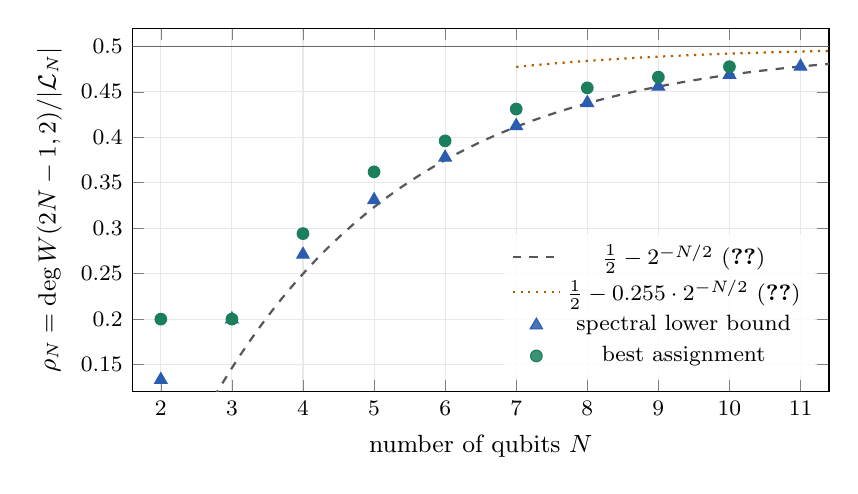
\begin{tikzpicture}
\begin{axis}[width=0.86\linewidth,height=6.2cm,xmin=1.6,xmax=11.4,ymin=0.12,ymax=0.52,
  xlabel={number of qubits $N$},ylabel={$\rho_N=\deg\W{2N-1}/|\Lines_N|$},
  xtick={2,...,11},ytick={0.15,0.2,0.25,0.3,0.35,0.4,0.45,0.5},
  yticklabel style={/pgf/number format/fixed,/pgf/number format/precision=2},
  legend style={at={(0.98,0.04)},anchor=south east,font=\footnotesize,draw=none,fill=white,fill opacity=0.85,text opacity=1},
  grid=major,grid style={gray!18},tick label style={font=\footnotesize},label style={font=\small}]
\addplot[domain=2:11.4,samples=60,thick,dashed,inkgray] {0.5-2^(-x/2)};
\addlegendentry{$\frac12-2^{-N/2}$ (\cref{thm:limit})}
\addplot[domain=7:11.4,samples=40,thick,dotted,numorange] {0.5-0.255*2^(-x/2)};
\addlegendentry{$\frac12-0.255\cdot2^{-N/2}$ (\cref{thm:rate})}
\addplot[only marks,mark=triangle*,mark size=2.6pt,certblue] coordinates
 {(2,0.1333)(3,0.2)(4,0.2710)(5,0.3310)(6,0.3778)(7,0.4126)(8,0.4379)(9,0.4559)(10,0.4688)(11,0.4779)};
\addlegendentry{spectral lower bound}
\addplot[only marks,mark=*,mark size=2.1pt,leangreen] coordinates
 {(2,0.2)(3,0.2)(4,0.2941)(5,0.3620)(6,0.3961)(7,0.4311)(8,0.4544)(9,0.4662)(10,0.4777)};
\addlegendentry{best assignment}
\addplot[thin,black!60] coordinates {(1.6,0.5)(11.4,0.5)};
\end{axis}
\end{tikzpicture}
\caption{The contextuality ratio of $\W{2N-1}$ is squeezed towards $\tfrac12$. The true value lies between each
triangle and the dot above it; for $N=3$ they coincide.}
\label{fig:rho}
\end{figure}

\subsection{Quadrics}

The same bound applies to the quadrics, which are induced configurations with $n=2^{N-1}(2^N\pm1)-1$ points. For
$N\ge3$ it gives
\[
  \deg\Qp7\ge315,\quad\deg\Qp9\ge6426,\quad\deg\Qm9\ge4873,
\]
\leancin{Qplus7\_eq\_315, Qp9\_ge\_6426, Qm9\_ge\_4873} and in general $\rho(Q^\pm(2N-1,2))\to\tfrac12$ with
$\tfrac12-\rho=O(2^{-N/2})$. The first of these is exact (\cref{thm:qp7}). The bound $6426>4743=|\Lines|/5$ answers
the question of~\cite{LiGuptaGanesh2026} for $\Qp9$ negatively. For $\Qm7$, however, the spectral bound gives only
$145$, much weaker than the combinatorial $216$ of \cref{thm:216}; \cref{sec:neg} explains why. We do not have a
matching upper rate for quadrics: the random-state argument gives $c^2\to1/\pi<\tfrac12$ and hence nothing.

%% ---- sec-tight.tex ----
%=====================================================================================================
\section{When the spectral bound is exact: Pauli-flat states}\label{sec:tight}
%=====================================================================================================

For $N=3$ the spectral bound for $\W5$ is exactly $63$, the true degree. This section explains when that happens.
The answer is a statement about quantum states, and it identifies optimal noncontextual assignments with
maximally magic states.

\begin{definition}
Let $X\subseteq\Vs$. A unit vector $\psi\in\C^d$ is \emph{Pauli-flat on $X$} if $|\ev{P_a}_\psi|$ is the same for
all $a\in X$ and $\ev{P_a}_\psi=0$ for all $a\in\Vs\setminus X$.
\end{definition}

By completeness (\cref{lem:pauli}(iv)), $\sum_{a\ne0}\ev{P_a}_\psi^2=d-1$, so the common value is forced to be
$\gamma=\sqrt{(d-1)/n}$ with $n=|X|$. A state flat on $X=\Vs$ has $|\ev{P_a}|^2=1/(d+1)$ for every non-identity
Pauli: it is a fiducial vector of a SIC-POVM covariant under the $N$-qubit Pauli group.

\subsection{The characterisation}

\begin{theorem}[tightness]\label{thm:tight}
Let $X\subseteq\Vs$ be an induced configuration on $N\ge1$ qubits with $n=|X|\ge1$. The following are equivalent:
\begin{enumerate}[label=(\roman*)]
\item $\displaystyle\deg X=\frac{|\Lines_X|}{2}-\frac{n^{3/2}(d-2)}{12\sqrt{d-1}}$, i.e.\ \eqref{eq:spectral} is
an equality;
\item some pure state is Pauli-flat on $X$.
\end{enumerate}
In that case the optimal assignments are exactly the sign patterns $g(a)=\sgn\ev{P_a}_\psi=\gamma^{-1}\ev{P_a}_\psi$
of the states $\psi$ that are flat on $X$, and for each optimal $g$,
\[
  M_g=\frac{d\,\proj{\psi}-I}{\gamma},\qquad\gamma=\sqrt{\frac{d-1}{n}} .
\]
\lean{tight\_of\_flat, tight\_converse, tight\_iff}
\end{theorem}

\begin{proof}
\emph{(ii)$\Rightarrow$(i).} Let $\psi$ be flat with $e_a=\ev{P_a}_\psi$ and put $g(a)=e_a/\gamma\in\{\pm1\}$ on $X$.
The Pauli expansion of \cref{lem:pauli}(iv) reads
$d\proj\psi=\sum_ae_aP_a=I+\sum_{a\in X}e_aP_a=I+\gamma M_g$, so $M_g=(d\proj\psi-I)/\gamma$. Its spectrum is
$\{(d-1)/\gamma\}\cup\{-1/\gamma\}^{d-1}$, and
\[
  \tr M_g^3=\frac{(d-1)^3-(d-1)}{\gamma^3}=\frac{d(d-1)(d-2)}{\gamma^3}=\frac{d\,n^{3/2}(d-2)}{\sqrt{d-1}} .
\]
By~\eqref{eq:trace}, $\viol(g)$ equals the right-hand side of~\eqref{eq:spectral}. Hence
$\text{bound}\le\deg X\le\viol(g)=\text{bound}$.

\emph{(i)$\Rightarrow$(ii).} Let $g$ be optimal, $M=M_g$, $\Lambda=\sqrt{n(d-1)}$, $F=dn$, $\mu=F/(d\Lambda)=n/\Lambda$.
By (i) and~\eqref{eq:trace}, $\tr M^3=B(\Lambda)$, so the inequality in the proof of \cref{thm:spectral} is an
equality: $\tr(BAB)=0$ with $A=\Lambda I-M\succeq0$ and $B=M+\mu I$. A positive semidefinite matrix with zero
trace vanishes, so $BAB=0$; then $(A^{1/2}B)^\dagger(A^{1/2}B)=0$, so $A^{1/2}B=0$ and $AB=0$:
\[
  (\Lambda I-M)(M+\mu I)=0 .
\]
Put $R=(M+\mu I)/(\Lambda+\mu)$. The displayed identity says $M(M+\mu I)=\Lambda(M+\mu I)$, hence $R^2=R$. So $R$
is a Hermitian idempotent, i.e.\ an orthogonal projection, and its rank is
$\tr R=d\mu/(\Lambda+\mu)=(dn/\Lambda)\big/(nd/\Lambda)=1$, using $\Lambda^2+n=nd$. Thus $R=\proj\psi$ for a unit
vector $\psi$ and $M=(\Lambda+\mu)\proj\psi-\mu I$. Now compare Pauli coefficients using
$\tr(P_aP_b)=d[a=b]$: for $a\ne0$,
\[
  \tr(MP_a)=(\Lambda+\mu)\,\ev{P_a}_\psi=\begin{cases}d\,g(a),&a\in X,\\0,&a\notin X.\end{cases}
\]
So $\ev{P_a}_\psi=d\,g(a)/(\Lambda+\mu)=g(a)\Lambda/n=\pm\gamma$ on $X$ and $0$ off $X$: $\psi$ is flat, and $g$ is
its sign pattern. Conversely, the first part shows that every sign pattern of a flat state is optimal.
\end{proof}

The formal proof follows exactly this route: no spectral theorem and no multiplicity count, only the trace of
$BAB$, idempotents and Pauli coefficients \leanin{cubic\_eq\_case, rank\_one\_of\_idem}.

\begin{corollary}[integrality]\label{cor:integrality}
If (i) holds, then $n^{3/2}(d-2)/(12\sqrt{d-1})\in\tfrac12\Z$. For instance, when $d-1$ is prime ($N=3,5,7,\dots$
Mersenne), $n$ must be $(d-1)$ times a square.
\end{corollary}
\begin{proof}
Both $\deg X$ and $|\Lines_X|/2$ lie in $\tfrac12\Z$.
\end{proof}

\begin{corollary}[the full space is tight only for $N=1,3$]\label{cor:Wnottight}
$\deg\W{2N-1}$ equals the bound of \cref{thm:limit} if and only if a Pauli-covariant SIC exists in dimension
$2^N$, which happens only for $N=1$ and $N=3$~\cite{GodsilRoy2009}. For $N\ge4$ the inequality of
\cref{thm:limit} is strict.
\end{corollary}

\subsection{Three qubits: optimal assignments are Hoggar fiducials}

\begin{theorem}[$\W5$ and the Hoggar lines]\label{thm:hoggar}
$\deg\W5=63$. The map $g\mapsto\proj\psi$ defined by $M_g=24\proj\psi-3I$ is a bijection from the optimal
assignments of $\W5$ onto the projectors $\proj\psi$ of unit vectors with $|\ev{P_a}_\psi|^2=\tfrac19$ for all
$63$ non-identity three-qubit Paulis, i.e.\ onto the fiducial projectors of Pauli-covariant SICs in $\C^8$.
Its inverse is $g(a)=3\ev{P_a}_\psi$.
\leanc{W5\_eq\_63}
\end{theorem}
\begin{proof}
For $N=3$, $n=63$ the bound~\eqref{eq:spectral} is $315/2-63^{3/2}\cdot6/(12\sqrt7)=157.5-94.5=63$, and an explicit
assignment violates $63$ lines \cert{D3}. So (i) of \cref{thm:tight} holds, with $\gamma=\tfrac13$, and the theorem
gives the bijection: $g$ determines $M_g$, hence $\proj\psi$, and $\proj\psi$ determines $g=3\ev{P_a}_\psi$.
\end{proof}

Two assignments with the same violated set differ by an element of the \emph{gauge space}
$K=\ker H\subseteq\F^{\Vs}$ of assignments that satisfy every line with sign $0$. For $\W5$ this space is larger
than one might guess.

\begin{proposition}[gauge space of $\W5$]\label{prop:gauge}
The $315\times63$ incidence matrix of $\W5$ has rank $56$ over $\F$, so $\dim K=7$. The space $K$ consists of the
$64$ linear functionals $a\mapsto\omega(b,a)$ and the $64$ quadratic forms polarising to $\omega$; the form
$q^+(a)=y(a)\bmod2$ is a non-linear element. Every violated set that is attained is attained by exactly $2^7=128$
assignments. \leanc{finrank\_kerW3, rank\_incW3, qplus\_mem\_kerW, card\_fiber\_violated}
\end{proposition}
\begin{proof}
A quadratic form $q$ polarising to $\omega$ satisfies $q(a)+q(b)+q(a+b)=\omega(a,b)=0$ on every line, so it lies in
$K$, and so does every linear functional; together they form a $7$-dimensional space. The rank $56$ is a finite
computation; in the formal proof it is certified by a $56$-step propagation from the seven points
$X_1,X_2,X_3,Z_1,Z_2,Z_3,Y_1$, each step using a line with two determined points. Two assignments with the same
violated set differ by an element of $K$.
\end{proof}

The two kinds of gauge have a quantum meaning. Replacing $\psi$ by $P_b\psi$ multiplies $\ev{P_a}$ by
$(-1)^{\omega(a,b)}$: a linear gauge. Replacing $\psi$ by its complex conjugate $\bar\psi$ multiplies $\ev{P_a}$ by
$(-1)^{y(a)}$ because $\bar P_a=(-1)^{y(a)}P_a$: the quadratic gauge. So a violated set of $\W5$ corresponds to a
conjugate pair of Pauli-covariant SICs. The $\Sp(6,2)$-orbit of one optimal violated set has $120$ elements, with
stabiliser of order $12096=|G_2(2)|$ \cert{X5}, and $4000$ random restarts of an ascent in state space found no
other optimal violated set. Assuming the classification of three-qubit Pauli-covariant SICs~\cite{Hoggar1998,
GodsilRoy2009}, every optimal violated set lies in this orbit, and the number of optimal assignments is
$120\cdot128=15360$ \cert{X14}. This is the number of three-qubit maximal-magic states found
in~\cite{ExtremalMagic2025}, which is a reassuring independent check. The appearance of $G_2(2)$ matches the split
Cayley hexagon picture of~\cite{Saniga2023}.

By transfer (\cref{thm:rigidity}), every optimal assignment of $\W5$ violates exactly $3$ lines of each of its $336$
doilies, $21$ of each hyperbolic and $9$ of each elliptic three-qubit quadric \leancin{doily\_rigid, Qp5\_rigid,
Qm5\_rigid}. In the language of states: a Hoggar fiducial, read as a $\pm1$ pattern, is simultaneously optimal on
every one of these sub-geometries.

\subsection{Four and five qubits}

\begin{theorem}[$\Qp7$]\label{thm:qp7}
$\deg\Qp7=315$. The real four-qubit state
\[
  \psi=\sqrt{\tfrac23}\bigl(\ket{+}^{\otimes4}-\ket{0}^{\otimes4}\bigr)=\tfrac1{\sqrt{24}}(-3,1,1,\dots,1)
\]
has $|\ev{P_a}_\psi|=\tfrac13$ on the $135$ symmetric non-identity Paulis and $\ev{P_a}_\psi=0$ on the $120$
antisymmetric ones, and the optimal assignments include its sign pattern.
\leanc{Qplus7\_eq\_315, Qplus7\_flat, Qplus7\_eq\_315\_flat}
\end{theorem}
\begin{proof}
$\Qp7$ is induced by the $135$ symmetric Paulis, and the bound~\eqref{eq:spectral} is
$1575/2-135^{3/2}\cdot14/(12\sqrt{15})=787.5-472.5=315$. For the state, an antisymmetric Pauli ($y(a)$ odd) has purely imaginary matrix entries
by~\eqref{eq:paulimatrix}, so a real state has $\ev{P_a}=0$ on it. For a symmetric $P_a\ne I$ write
$\psi=\sqrt{2/3}\,(u-w)$ with $u=\ket+^{\otimes4}$ and $w=\ket0^{\otimes4}$, so that $\braket uw=\tfrac14$ and
$\|u-w\|^2=\tfrac32$. Then
\[
  \tfrac32\ev{P_a}_\psi=\bra uP_a\ket u-2\,\mathrm{Re}\bra uP_a\ket w+\bra wP_a\ket w .
\]
Here $\bra uP_a\ket u=1$ if $P_a$ is a product of $X$'s and identities and $0$ otherwise; $\bra wP_a\ket w=1$ if $P_a$
is a product of $Z$'s and identities and $0$ otherwise; and $\bra uP_a\ket w=\tfrac14i^{y(a)}=\tfrac14(-1)^{y(a)/2}$.
If $P_a$ is a non-trivial product of $X$'s, or of $Z$'s, the right-hand side is $1-\tfrac12=\tfrac12$; otherwise it
is $\mp\tfrac12$. In all cases $|\ev{P_a}_\psi|=\tfrac13$ \cert{X12}, and \cref{thm:tight} applies.
\end{proof}

Li, Gupta and Ganesh proved $\deg\Qp7=315$ first, by a SAT-certified classification~\cite{LiGuptaGanesh2026}; the
proof above is independent and short, and it identifies the optimum. The vector $(-3,1,\dots,1)/\sqrt{24}$ was found
numerically by Cie\'sli\'nski~\cite{Cieslinski2026} as a state with $135$ equal non-zero Pauli expectations.
\Cref{thm:qp7} gives it a combinatorial meaning: its sign pattern is an optimal noncontextual assignment of the
four-qubit hyperbolic quadric, and its stabiliser-$L^1$ norm is exactly what the contextuality degree measures.

\begin{theorem}[a five-qubit configuration with degree $480$]\label{thm:x496}
There is a set $X_{496}$ of $496$ five-qubit Pauli labels whose induced configuration has $10880$ lines and degree
exactly $480$. Its points lie on $60$, $64$ or $68$ lines, so it is not a homogeneous geometry.
\leanc{X496\_lines, X496\_eq\_480}
\end{theorem}
\begin{proof}
For $n=496$ and $d=32$ we have $\Lambda=\sqrt{496\cdot31}=124$, an integer, and
$n^{3/2}(d-2)/(12\sqrt{d-1})=496\cdot\sqrt{16}\cdot30/12=4960$. So~\eqref{eq:spectral} gives
$\deg X_{496}\ge5440-4960=480$. The sign pattern of a numerically flat state violates exactly $480$ lines, counted
directly \cert{X13}.
\end{proof}

The degree of $X_{496}$ does not depend on the flat state being exactly flat: the bound is an exact rational number
and the witness is counted. The state we store is flat to within $10^{-4}$ ($|\ev{P_a}|=\tfrac14$ on $X_{496}$, $0$
off it), and its support type is the $496$-element support found in~\cite{Cieslinski2026}. We do not know a closed
form for it, and the family may contain nicer members.

\subsection{Limits of the single-eigenvalue method}\label{sec:neg}

For $\Qm7$ the spectral bound is $145$, while $\deg\Qm7\ge216$ by a combinatorial argument. Could a better choice
of $\Lambda$ in \cref{thm:spectral} close the gap? No: the bound is monotone in $\Lambda$, so its best possible value
is reached at $\Lambda^*(X)$ from~\eqref{eq:lambdastar}, and any explicit state caps it.

\begin{proposition}[ceiling of the spectral method]\label{prop:ceiling}
For every valid $\Lambda$ and every unit vector $v$, $\Lambda\ge\sum_{a\in X}|\ev{P_a}_v|$, hence \cref{thm:spectral}
can never prove more than $|\Lines_X|/2-B\bigl(\sum_{a\in X}|\ev{P_a}_v|\bigr)/(12d)$.
\lean{valid\_ge\_rayleigh, ceiling}
\end{proposition}

Explicit states give the following ceilings \cert{X17}. On $\Qm7$, a state with $\sum_{a\in\Qm7}|\ev{P_a}|\ge28.18$
caps the method at $297$; the Cauchy--Schwarz value $\sqrt{119\cdot15}=42.25$ is far from it. On $\W7$, the state
behind the $1575$ witness has $\lambda_{\max}=21+16\sqrt6\approx60.19$, which caps the method at $1488$. On $\Qp9$ and
$\W9$ the caps are $6589$ and $29594$. The ratio between the best state and the Cauchy--Schwarz value is $1.000$
on $\Qp7$, $0.973$ on $\W7$ and only $0.667$ on $\Qm7$: elliptic quadrics admit no state that is anywhere near flat,
and the single-eigenvalue method cannot see the obstruction that the combinatorial certificate uses. Two-class
weighted versions (constant weights on $\Qm7\cap a^\perp$ and on the rest, or on $\Qm7$ and its complement in $\W7$)
combined with the combinatorial bounds in a linear program give no gain.

Two natural improvements remain. The first is a non-trivial \emph{upper} bound on $\Lambda^*(\Qm7)$, a polynomial
optimisation over the unit sphere of $\C^{16}$ that is in principle accessible to sum-of-squares certificates;
$\Lambda^*(\Qm7)\le28.19$ would give $\deg\Qm7\ge298$. The second is to use more than one eigenvalue: the $1575$
witness of $\W7$ has spectrum $\{21\pm16\sqrt6,(-3)^{14}\}$, so $M+3I$ has rank two, and the conjectured optimum of
$\Qm7$ shows the same pattern.

\begin{conjecture}[magic conjecture]\label{conj:magic}
The optimal assignments of $\W{2N-1}$ are sign patterns $\sgn\ev{P_a}_\psi$ of states $\psi$ maximising the Pauli
$L^1$ norm $\sum_a|\ev{P_a}_\psi|$.
\end{conjecture}
\emph{Evidence.} The conjecture holds for $N=3$ by \cref{thm:hoggar}. An alternating ascent
$\psi\mapsto g=\sgn\ev{P}_\psi\mapsto$ top eigenvector of $M_g$ reproduces the best known values $3,63,1575,31479$
for $N=2,\dots,5$, with $\lambda_{\max}=3+2\sqrt3$, $21$, $21+16\sqrt6$ and $168.90$; restricted to quadrics it
reproduces $21,315,6975$ ($\Qp5,\Qp7,\Qp9$) and $9,315$ ($\Qm5,\Qm7$). For $N\ge6$ the plain ascent does worse than
tensor products, so either the conjecture fails there or the search is too weak.

%% ---- sec-games.tex ----
%=====================================================================================================
\section{Nonlocal games}\label{sec:games}
%=====================================================================================================

The parity inequality of \cref{prop:operational} is a single-system test, and it inherits the usual loopholes of
sequential measurements. A two-player version avoids them.

\subsection{The game of a configuration}

Let $C$ be a configuration of $N$-qubit Paulis with three-element contexts. Its linear-system game $G_C$, in the
sense of Cleve and Mittal~\cite{CleveMittal2014}, is played as follows. The referee picks a line $\ell\in\Lines(C)$
uniformly at random and sends it to Alice, and picks a point $p\in\ell$ uniformly at random and sends it to Bob.
Alice answers three bits $(x_a)_{a\in\ell}$ with $\sum_{a\in\ell}x_a=e(\ell)$; Bob answers one bit $y$. They win if
$y=x_p$.

\begin{theorem}[classical and quantum value]\label{thm:game}
\begin{enumerate}[label=(\roman*)]
\item The classical value is $\omega_c(G_C)=1-\dfrac{\deg C}{3|\Lines(C)|}$. Shared randomness does not help.
\item If $C$ is induced, or more generally if its signs are the Pauli signs, the quantum value is $1$: Alice and
Bob share $N$ EPR pairs, Alice measures the commuting observables $P_a$, $a\in\ell$, and Bob measures $P_p^{\mathsf T}$.
\end{enumerate}
\lean{classicalValue\_eq, mixture\_le, quantum\_perfect}
\end{theorem}

\begin{proof}
(i) A mixed strategy is a convex combination of deterministic ones, so it suffices to consider those
\leanin{mixture\_le}. A deterministic Bob is an assignment $x:\Pts(C)\to\F$. If $x$ satisfies $\ell$, Alice answers
$x|_\ell$ and wins with probability $1$. If $x$ violates $\ell$, every admissible answer of Alice differs from
$x|_\ell$ in an odd number of positions, hence in at least one, and an answer at distance one exists; she wins with
probability $\tfrac23$ \leanin{agree\_le\_of\_violated}. The winning probability of the pair is
$1-\viol(x)/(3|\Lines(C)|)$, maximised by an optimal assignment.

(ii) Let $\ket\Phi=d^{-1/2}\sum_c\ket c\ket c$. For any matrices $A,B$,
$\bra\Phi A\otimes B^{\mathsf T}\ket\Phi=\tr(AB)/d$ \leanin{epr\_expect}. Alice's joint measurement of the commuting
$P_a,P_b,P_c$ has outcomes whose product is the eigenvalue of $P_aP_bP_c=(-1)^{e(\ell)}I$, so her answers are always
admissible \leanin{alice\_valid}. If Bob measures $P_p^{\mathsf T}$, the joint outcome distribution of $(P_p,
P_p^{\mathsf T})$ on $\ket\Phi$ is perfectly correlated, since $\bra\Phi\Pi\otimes\Pi'^{\mathsf
T}\ket\Phi=\tr(\Pi\Pi')/d$ for the spectral projectors. The formal statement computes these probabilities for every
line and every outcome.
\end{proof}

Since some assignment satisfies at least half of the equations of any system~\eqref{eq:half}, every three-variable
linear-system game has $\omega_c\ge\tfrac56$ \leanin{classicalValue\_ge}. This floor is folklore and is stated
in~\cite{TallerVidick2025}.

\subsection{The symplectic family reaches the floor}

\begin{theorem}[the $\W{2N-1}$ games]\label{thm:gameW}
Let $G_N$ be the game of $\W{2N-1}$. Then $\omega_q(G_N)=1$ with $N$ EPR pairs, and
\[
  \omega_c(G_N)=1-\frac{\rho_N}3=\frac56+\frac{\delta_N}3,\qquad
  \frac56+\frac{\kappa(2^{N-2})}6\ \le\ \omega_c(G_N)\ \le\ \frac56+\frac{2^{-N/2}}3 .
\]
In particular $\omega_c(G_N)\downarrow\tfrac56$. The first values are $\omega_c(G_2)=\omega_c(G_3)=\tfrac{14}{15}$,
$\omega_c(G_4)\in[0.9019,0.9097]$ and $\omega_c(G_5)\in[0.8793,0.8897]$.
\lean{W\_value\_eq, W\_value\_le, W\_value\_tendsto}
\end{theorem}
\begin{proof}
\Cref{thm:game} and \cref{thm:limit,thm:kendall}; monotonicity is \cref{cor:extremal}. The numerical values
use \cref{tab:rho}.
\end{proof}

To our knowledge, this is the first explicit family of linear-system games with perfect quantum strategies whose
classical value tends to the minimum possible value $\tfrac56$. The gap $1-\omega_c\to\tfrac16$ is the largest
possible in this class, and it is reached with Pauli measurements on $N$ EPR pairs. The rate is also optimal for
Pauli strategies:

\begin{corollary}[dimension--gap law]\label{cor:gap}
Every linear-system game with three-variable equations that has a perfect quantum strategy given by an $N$-qubit
Pauli operator solution satisfies
\[
  1-\omega_c\ \le\ \frac{1-\kappa(2^{N-2})}{6}=\frac16-\Theta\bigl(2^{-N/2}\bigr).
\]
The $\W{2N-1}$ game achieves $1-\omega_c\ge\tfrac16-\tfrac13 2^{-N/2}$. So the optimal classical--quantum gap with
$N$ EPR pairs and Pauli strategies is $\tfrac16-\Theta(2^{-N/2})$. \paperonly
\end{corollary}
\begin{proof}
Replacing an operator $\pm P_a$ by $P_a$ flips the corresponding variable, which does not change the classical
value. An equation whose three operators are three distinct non-identity Paulis is a line of $\W{2N-1}$ with its
Pauli sign, and the measure-and-assign strategy of \cref{thm:kendall} satisfies it with probability
$(1+\kappa(2^{N-2}))/2$. Any other equation (one involving the identity, or a repeated operator) is satisfied by that
strategy with probability one, because $g(I)=1$ and repeated operators receive equal values. Averaging over
equations and using \cref{thm:game}(i) for the game gives the bound.
\end{proof}

For comparison, the magic square game has gap $\tfrac19$ in its row--column format~\cite{Lau2026}; in our
equation--variable format the Peres--Mermin square has $\omega_c=\tfrac{17}{18}$ and the doily $\tfrac{14}{15}$
\cert{X15}. Values in different formats should not be compared directly.

\subsection{Noise and the number of rounds}

\begin{proposition}[noise]\label{prop:noise}
Suppose the players share $v\proj\Phi^{\otimes N}+(1-v)I/d^2$ and use the strategy of \cref{thm:game}(ii). Then
they win with probability $(1+v)/2$. Hence the game certifies nonlocality as soon as $v>1-\tfrac23\rho(C)$, a
threshold that tends to $\tfrac23$ for the $\W{2N-1}$ family. \paperonly
\end{proposition}
\begin{proof}
On the maximally mixed part Alice's answers are still admissible and Bob's bit is uniform and independent, so they
agree with probability $\tfrac12$; on the EPR part they agree with probability $1$. The win probability
$(1+v)/2$ exceeds $\omega_c=1-\rho/3$ iff $v>1-2\rho/3$.
\end{proof}

The single-system parity test of \cref{prop:operational} tolerates much more noise: its attenuation threshold
$1-2\rho_N\le2^{1-N/2}$ is exponentially small. But it assumes that sequential measurements are compatible and
non-disturbing, and the nonlocal version does not. We keep the two statements separate.

\begin{proposition}[constant number of rounds]\label{prop:rounds}
Play $T$ rounds of $G_C$ with fresh, independent, uniformly random questions, and let $W_T$ be the fraction of rounds
won. Against every classical strategy, including strategies that adapt to the history of previous rounds,
\[
  \Pr\bigl[W_T\ge\omega_c(G_C)+\eps\bigr]\ \le\ e^{-2T\eps^2}.
\]
For $G_N$ with ideal devices one may take $\eps=\tfrac16-\tfrac132^{-N/2}-\eta$ for any slack $\eta>0$, so
$T=O(\log(1/\eta'))$ rounds distinguish quantum from classical players with error $\eta'$, independently of $N$ and
of the number of contexts. \paperonly
\end{proposition}
\begin{proof}
Conditioned on the history, the questions of round $t$ are fresh and uniform, and a classical strategy for round $t$
is a (history-dependent) classical strategy for one copy of the game; its conditional winning probability is at
most $\omega_c$. The centred indicators form a supermartingale difference sequence with increments in $[-1,1]$
shifted to an interval of length one, and the Azuma--Hoeffding inequality gives the bound.
\end{proof}

One could instead fix $m$ contexts in advance and estimate their correlators. Then a union bound over all
assignments gives a deviation term of order $\sqrt{n/m}$, which needs $m\gtrsim n2^N$ contexts. Fresh random
questions in every round avoid this cost entirely. The same martingale argument applies to the single-system
parity test against noncontextual models without memory; memory-assisted models are the known
loophole~\cite{Kleinmann2011}.

%% ---- sec-geometry.tex ----
\section{Small geometries, sections and the elliptic quadric}\label{sec:geometry}
%=====================================================================================================

This section collects exact results on specific geometries. Some re-derive known values in a way that yields more
information (statements about \emph{all} configurations and \emph{all} optimal assignments); the rest are new.

\subsection{Three qubits}\label{sec:three}

The exact degrees in this subsection were computed by SAT solving in~\cite{deBoutray2022,Muller2024}, and the
unsatisfied lines of optimal assignments were described geometrically in~\cite{Muller2024,Saniga2023}. We
re-derive them from transfer for two reasons: to keep the paper self-contained, and because transfer yields
statements about \emph{all} configurations and \emph{all} optimal assignments (\cref{thm:3qubit,cor:3rigid}).

\begin{proposition}\label{prop:doily}
The Peres--Mermin square has degree $1$, the doily $\W{3}$ has degree $3$, and $\W{5}$ has degree $63$.
Hence $\rho_2=\rho_3=\frac15$.
\leanc{grid\_odd, W3\_eq\_3, W5\_eq\_63}
\end{proposition}
\begin{proof}
\emph{Square.} A set of rows and columns covering each of the nine points an even number of times contains row $i$
iff it contains column $j$, for all $i,j$; so the cycle space is spanned by the set of all six lines, which has odd
parity \cert{D2}. By~\eqref{eq:coset} the degree is the distance from an odd-weight vector to the even-weight code,
namely $1$.
\emph{Doily.} The square is a sub-configuration of $\W{3}$ and $\Sp(4,2)$ is line-transitive, so
Theorem~\ref{thm:transfer} gives $\deg\W3\ge\lceil 15/6\rceil=3$; the all-zero assignment violates exactly the three
lines of sign $1$ \cert{D1}.
\emph{$\W5$.} Embedding the doily (by padding) and applying \cref{thm:transfer} gives $\deg\W5\ge315\cdot
3/15=63$ (this is the second proof; the first is \cref{thm:hoggar}); an explicit assignment violating $63$ lines is
given in the certificate \cert{D3}.
\end{proof}

\begin{theorem}[three-qubit bound]\label{thm:3qubit}
Every configuration $S$ on at most three qubits satisfies $\deg S\le\lfloor|\Lines(S)|/5\rfloor$. Equality
$\deg S=|\Lines(S)|/5$ holds for the doily, for $\W5$, and for both quadrics $\Qp5$ (degree $21$) and $\Qm5$
(degree $9$).
\leanc{three\_qubit\_bound, Qp5\_eq\_21, Qm5\_eq\_9}
\end{theorem}
\begin{proof}
The bound is Corollary~\ref{cor:extremal}(i) with $\rho_3=\frac15$. For the quadrics: for a point $a$ with $q(a)=1$, the hyperplane section $D=a^\perp$ is a parabolic quadric $Q(4,2)$
with $15$ points and $15$ lines. The radical of $\omega|_D$ is $\langle a\rangle$, and since
$q(p+a)=q(p)+1$ for $p\in D$, the projection $D\to D/\langle a\rangle\cong\F^4$ maps its points bijectively onto
the points of $\W3$, preserving $\omega$ and lines; by Corollary~\ref{cor:invariance} it has degree $3$; with $\Orth(q^\pm)$ line-transitive,
Theorem~\ref{thm:transfer} gives $\deg\Qp5\ge105/5=21$ and $\deg\Qm5\ge45/5=9$. The optimal $\W5$ assignment of
\cert{D3} violates exactly $21$ lines of every hyperbolic and $9$ of every elliptic quadric \cert{R1}, giving the
matching upper bounds.
\end{proof}

\begin{corollary}[three-qubit rigidity]\label{cor:3rigid}
Every optimal assignment of $\W5$ violates exactly $3$ lines of each of its $336$ doilies, exactly $21$ lines of
each of its $36$ hyperbolic quadrics and exactly $9$ lines of each of its $28$ elliptic quadrics.
\leanc{doily\_rigid, Qp5\_rigid, Qm5\_rigid}
\end{corollary}
\begin{proof}
Theorem~\ref{thm:rigidity}(a)$\Rightarrow$(b), since all three ratios equal $\rho_3=\frac15$, and $\Sp(6,2)$ is
transitive on non-degenerate $4$-spaces and on quadratic forms of each type polarising to $\omega$. (The
certificate confirms the statement on one optimal assignment \cert{R1, R2}; this is a consistency check, not part
of the proof.) The statement is compatible with the descriptions of optimal unsatisfied sets of the individual
quadrics in~\cite{Muller2024}: a spread of $9$ lines for each elliptic quadric, and a Heawood-graph configuration
of $21$ lines for each hyperbolic one.
\end{proof}

\subsection{Cones and sections: exact degrees}\label{sec:cones}
%=====================================================================================================

The tangent hyperplane sections of $\W{2N-1}$ and of the quadrics are not line-transitive (the lines through the
point of tangency form a separate orbit), so Theorem~\ref{thm:transfer} does not apply to them directly. They are
cones, and their degrees can be computed exactly.

\begin{definition}[cones]
Let $G'$ be a configuration on $n$ qubits and $t\ge1$. Write points of $n+t$ qubits as $v\otimes Z^{\tau}$ with
$v\in\F^{2n}$ and $\tau\in\F^{t}$ (a $Z$-type operator on the last $t$ qubits). The \emph{cone} $\mathrm{Cone}_t(G')$
has the following lines:
\begin{enumerate}[label=(\alph*)]
\item \emph{lifts} $\{a\otimes Z^{\alpha},\,b\otimes Z^{\beta},\,c\otimes Z^{\alpha+\beta}\}$ for each line
$\{a,b,c\}$ of $G'$ and $\alpha,\beta\in\F^t$ ($4^t$ lifts per line);
\item \emph{vertex lines} $\{v\otimes Z^{\tau},\,v\otimes Z^{\tau'},\,I\otimes Z^{\tau+\tau'}\}$ for
$v\in P'$ and $\tau\neq\tau'$, where $P'\supseteq\Pts(G')$ is a fixed finite set of points (by default
$P'=\Pts(G')$; a larger $P'$ is needed when the base contains points on no line of $G'$);
\item \emph{lines in the vertex} $\{Z^{\tau},Z^{\tau'},Z^{\tau+\tau'}\}$ for distinct non-zero
$\tau,\tau'$ (when $t\ge2$).
\end{enumerate}
\end{definition}

\begin{theorem}[cone theorem]\label{thm:cone}
$\deg\mathrm{Cone}_t(G')=4^t\deg G'$. More precisely, the lines of types (b) and (c) have sign $0$ and can always
be satisfied simultaneously with an optimal choice on the lifts.
\lean{Config.cone\_degree, cone\_degree\_pauli, std\_sub\_degree}
\end{theorem}
\begin{proof}
\emph{Signs.} The canonical operator of $v\otimes Z^\tau$ is $P(v)\otimes Z^\tau$, since no $Y$ is created. A lift
has product $P(a)P(b)P(c)\otimes Z^{0}=(-1)^{e(abc)}I$, so it carries the sign of its base line; vertex lines have
product $P(v)^2\otimes Z^{0}=I$; lines in the vertex are $Z$-type. All signs of types (b) and (c) are therefore $0$.

\emph{Upper bound.} Given an optimal assignment $y$ of $G'$, extended by $0$ to $P'\setminus\Pts(G')$, put
$x(v\otimes Z^\tau)=y(v)$ and $x(Z^\tau)=0$. Lines
of types (b) and (c) are satisfied, and a lift is violated iff its base line is; the number of violated lines is
$4^t\deg G'$.

\emph{Lower bound.} Let $U=\operatorname{span}\Pts(G')$, $d=\dim U\ge2$, and for each linear
$\varphi:U\to\F^t$ let $\Sigma_\varphi$ be the sub-configuration of lifts with $\alpha=\varphi(a)$, $\beta=\varphi(b)$
(then the third exponent is $\varphi(c)$). The map $v\mapsto v\otimes Z^{\varphi(v)}$ is injective, preserves
$\omega$ (the $Z$-parts commute with everything in the cone) and maps lines of $G'$ onto lines of $\Sigma_\varphi$;
by Corollary~\ref{cor:invariance}, $\deg\Sigma_\varphi=\deg G'$. A given lift lies in $\Sigma_\varphi$ iff
$\varphi(a)=\alpha$ and $\varphi(b)=\beta$; as $a,b$ are linearly independent, this holds for exactly $2^{t(d-2)}$ of
the $2^{td}$ maps $\varphi$. For an assignment with violated set $V$, averaging over $\varphi$ gives
$|V|\ge|V\cap\text{lifts}|=4^{t}\cdot2^{-td}\sum_\varphi|V\cap\Sigma_\varphi|\ge4^t\deg G'$.
\end{proof}

The lower bound is the profile bound (Theorem~\ref{thm:profile}) for the group of shears
$v\otimes Z^\tau\mapsto v\otimes Z^{\tau+\psi(v)}$, whose line orbits are the classes of $4^t$ lifts of each line
of $G'$ together with the vertex lines. The cone has ratio
$\rho=4^t\deg G'/(4^t|\Lines(G')|+|\text{vertex lines}|)<\rho(G')$, so cones never help as transfer witnesses,
but their degrees are now known exactly.

\begin{theorem}[sections of the symplectic polar space]\label{thm:Wsections}
Let $X\subseteq\F^{2N}$ be a subspace, $R=X\cap X^\perp$ its radical, $t=\dim R$ and $2k=\dim X-t$. The
configuration $W(X)$ of all lines of $\W{2N-1}$ contained in $X$ satisfies
\[
\deg W(X)=4^{t}\,\deg\W{2k-1}\qquad(\text{with }\deg\W1=0).
\]
\lean{W\_section\_degree}
\end{theorem}
\begin{proof}
Write $X=R\oplus X_0$ with $X_0$ non-degenerate of dimension $2k$ (a symplectic basis adapted to the radical can be
built by splitting off one hyperbolic pair at a time, which is how the formal proof avoids Witt's theorem
\leanin{exists\_sympData}). Choose a symplectic basis of $X_0$ and a basis
$r_1,\dots,r_t$ of $R$; the linear map sending them to the standard symplectic basis of the first $k$ qubits and to
$Z_{k+1},\dots,Z_{k+t}$ is an isometry of $X$ onto $\F^{2k}\oplus\langle Z_{k+1},\dots,Z_{k+t}\rangle$, and it maps
the commuting zero-sum triples of $X$ to those of the image. In the image, a commuting zero-sum triple
$\{u_1\otimes Z^{\tau_1},u_2\otimes Z^{\tau_2},u_3\otimes Z^{\tau_3}\}$ has $u_1+u_2+u_3=0$ with the $u_i$ pairwise
commuting, so either all $u_i$ vanish (type (c)), or exactly two coincide and the third vanishes (type (b)), or the
$u_i$ form a line of $\W{2k-1}$ (type (a)). Hence the image is exactly $\mathrm{Cone}_t(\W{2k-1})$ with $P'=\F^{2k}\setminus\{0\}$, and
Corollary~\ref{cor:invariance} and Theorem~\ref{thm:cone} give the claim. (For $k\le1$ there are no lifts and all
lines have sign $0$.)
\end{proof}

\begin{theorem}[sections of quadrics]\label{thm:Qsections}
Let $q$ be a non-degenerate quadratic form on $\F^{2N}$ polarising to $\omega$, $X$ a subspace with radical $R$ of
$\omega|_X$, $t=\dim R$ and $2k=\dim X-t$. Since $\omega$ vanishes on $R$, $q|_R$ is linear.
\begin{enumerate}[label=(\alph*)]
\item If $q|_R=0$, then $\deg(X\cap Q)=4^{t}\deg Q^{\delta}(2k-1,2)$, where $\delta$ is the type of $q$ on a
complement $X_0$ of $R$ in $X$.
\item If $q|_R\neq0$, then $\deg(X\cap Q)=4^{t-1}\deg\W{2k-1}$.
\end{enumerate}
In particular every tangent hyperplane section of $Q^{\varepsilon}(2N-1,2)$ has degree
$4\deg Q^{\varepsilon}(2N-3,2)$, and every non-tangent one has degree $\deg\W{2N-3}$. Moreover the degree of a
non-degenerate quadric depends only on its type: every $q$ polarising to $\omega$ is $q^++\omega(c,\cdot)$ for a
unique $c$, and the transvection $x\mapsto x+\omega(d,x)d$ with $q(d)=0$ maps $q$ to $q+\omega(d,\cdot)$, so one
transvection moves $q$ to $q^+$ or to a fixed elliptic form according to $q^+(c)$; this is the Arf invariant
without its name \leanin{quad\_eq\_qplus\_add, quad\_tvL, deg\_secQ\_type}.
\lean{Q\_section\_degree\_a, Q\_section\_degree\_b, deg\_secQ\_type}
\end{theorem}
\begin{proof}
Write $X=R\oplus X_0$ with $X_0$ non-degenerate; $q(r+x)=q(r)+q(x)$ for $r\in R$, $x\in X$, since $\omega(r,x)=0$.
(a) The singular points of $X$ are $r+y$ with $y$ singular in $X_0$ or $y=0$ ($r\neq0$). An isometry
$X_0\to(\F^{2k},q^{\delta})$ together with $R\to\langle Z_{k+1},\dots,Z_{k+t}\rangle$ maps $X\cap Q$
onto the points of $\mathrm{Cone}_t(Q^\delta(2k-1,2))$ (with $P'$ the set of all singular points of $X_0$), and, by the same case analysis as in
Theorem~\ref{thm:Wsections} applied to singular triples, lines onto lines.
(b) Let $R_s=\ker(q|_R)$, of dimension $t-1$, and $r_0\in R$ with $q(r_0)=1$. Then $X=R_s\oplus Y$ with
$Y=\langle r_0\rangle\oplus X_0$, and the singular points of $X$ are $s+y$ with $s\in R_s$ and $y$ singular in $Y$ or
$y=0$. Every singular $y\in Y$ is $\epsilon r_0+x$ with $x\in X_0$, $\epsilon=q(x)$; so $y\mapsto x$ is a bijection
from the singular points of $Y$ onto $X_0\setminus\{0\}$. It preserves $\omega$ ($r_0$ is in the radical) and maps
singular lines to lines: if $y_1,y_2$ are singular and commute, then $y_1+y_2$ is singular and is the lift of
$x_1+x_2$. Hence the singular points of $Y$ form a configuration isometric to $\W{2k-1}$ (the parabolic quadric), and
$X\cap Q$ is, as in (a), isometric to $\mathrm{Cone}_{t-1}$ of it. Apply Theorem~\ref{thm:cone}. For a tangent
hyperplane $X=p^\perp$ ($q(p)=0$): $R=\langle p\rangle$, $q|_R=0$, and $X_0$ has the type of $q$. For a non-tangent one
($q(p)=1$): case (b) with $t=1$.
\end{proof}

\begin{table}[h]
\centering\small
\renewcommand{\arraystretch}{1.1}
\begin{tabular}{@{}lll@{}}
\toprule
section & degree & value\\\midrule
tangent hyperplane of $\W5$ & $4\deg\W3$ & $12$\\
tangent hyperplane of $\W7$, $\Qp7$, $\Qm7$ & $4\cdot63$, $4\cdot21$, $4\cdot9$ & $252$, $84$, $36$\\
non-tangent hyperplane of $\Qp7$, $\Qm7$ & $\deg\W5$ & $63$\\
tangent hyperplane of $\Qp9$ & $4\deg\Qp7$ & $\mathbf{1260}$\\
non-tangent hyperplane of $\Qp9$, $\Qm9$ & $\deg\W7$ & $[1451,1575]$\\
tangent hyperplane of $\W9$, $\Qm9$ & $4\deg\W7$, $4\deg\Qm7$ & $[5804,6300]$, $[864,1260]$\\\bottomrule
\end{tabular}
\caption{Exact degrees of hyperplane sections (\cref{thm:Wsections,thm:Qsections}). The four-qubit values are also
attained by lifted assignments \cert{K2}, and the smallest cone is checked exhaustively \cert{K1}. The
exact values are Lean theorems (\lname{W5\_tangent}, \lname{W7\_tangent}, \lname{tangent\_Qplus7},
\lname{tangent\_Qminus7}, \lname{Qplus7\_nontangent}, \lname{tangent\_Qplus9}). Every subspace
section of $\W9$ and of the five-qubit quadrics has its degree determined by the two unknowns $\deg\W7$ and
$\deg\Qm7$.}
\label{tab:sections}
\end{table}

\subsection{The elliptic quadric \texorpdfstring{$\Qm7$}{Q-(7,2)}}\label{sec:qm7}

The four-qubit elliptic quadric is the smallest geometry whose degree is unknown, and by
\cref{prop:collapse} below it controls several others. It has $119$ points and $1071$ lines; the averaging bound
over doilies gives $\deg\Qm7\ge\lceil1071/5\rceil=215$~\cite{LiGuptaGanesh2026}, the spectral bound only $145$, and
tabu search finds assignments with $315$ violated lines. We push the lower bound to $216$ with a certificate that
uses nothing but odd grids and the uniform cover lemma.

\begin{theorem}[an integrality cascade]\label{thm:216}
$\deg\Qm7\ge216$. \leanc{Qminus7\_bounds, qm7\_ge\_216}
\end{theorem}

\begin{proof}
All counts below are finite facts, verified both by the Python checker \cert{A1--A4} and inside Lean by a single
Boolean certificate evaluated with \texttt{native\_decide}.

\emph{Step 1: grids.} A grid (Peres--Mermin square) is a set of six lines in two parallel classes of three. Its six
lines form a cycle, and when its sign sum is odd it has degree $1$ (\cref{prop:doily}).

\emph{Step 2: doilies.} Let $c$ be non-singular ($q^-(c)=1$) and let $W\ni c$ be a $3$-space with radical $\langle
c\rangle$; there are $136\cdot336=45696$ such $W$. Then $U=W^\perp$ is a $5$-space with the same radical, and
$U\cap\Qm7$ is a parabolic quadric $Q(4,2)$; projecting along $c$ identifies it with $\W3$, so it is a doily
(\cref{thm:Qsections}(b)). In each of these doilies, the $60$ unordered pairs of disjoint lines span $60$ grids, counted with
multiplicity (each of its $10$ grids arises from six pairs), all of them odd, and every line of the doily lies in at most $24$ of them. By \cref{lem:cover}
every doily has degree at least $\lceil60/24\rceil=3$.

\emph{Step 3: the configurations $O_a$.} For a non-singular vector $a$ ($q^-(a)=1$; there are $136$) let $O_a$ be the
configuration of the $756$ lines of $\Qm7$ not contained in the hyperplane $a^\perp$. Exactly $4032$ doilies have all
their lines in $O_a$, and they cover each line of $O_a$ at most $80$ times. By \cref{lem:cover},
$\deg O_a\ge\lceil4032\cdot3/80\rceil=\lceil151.2\rceil=152$.

\emph{Step 4: the quadric.} The $136$ configurations $O_a$ cover each line of $\Qm7$ exactly $96$ times (a line
$\ell$ lies in $a^\perp$ iff $\omega(a,\cdot)$ vanishes on the plane spanned by $\ell$, which happens for $40$ of
the $136$ vectors $a$). By \cref{lem:cover},
$\deg\Qm7\ge\lceil136\cdot152/96\rceil=\lceil215.33\rceil=216$.
\end{proof}

The argument rounds up twice, and the gain over $215$ comes from the first rounding, which happens in a
configuration that is not three-qubit realisable; this is how it escapes the barrier of \cref{cor:barrier}. With
group theory one can say more: the stabiliser of $a$ in $\Orth(q^-)$ acts transitively on the lines of $O_a$ (by
Witt's extension theorem, or by explicit reflections \cert{A2}), so Step 3 is an instance of \cref{thm:transfer}.
The formal proof uses only the counts. A systematic search over about $1000$ line orbits of reflection subgroups of
$\Orth^-(8,2)$, iterating such roundings to a fixed point, found nothing better than $216$, and the profile integer
program of \cref{thm:profile} for the stabilisers of an anisotropic plane, a non-singular point and a singular
point, fed with about $9700$ witnesses of known degree, has value exactly $215$.

\begin{proposition}[collapse]\label{prop:collapse}
Through transfer, $\deg\W7\ge5\deg\Qm7$ and $\deg\Qp9\ge\lceil23715\deg\Qm7/1071\rceil$. In particular, if
$\deg\Qm7=315$ then $\deg\W7=1575$ and $\deg\Qp9=6975$, and all three have ratio $\tfrac5{17}$.
\end{proposition}
\begin{proof}
$\Qm7$ is a sub-configuration of $\W7$, and it embeds into $\Qp9$ as the section by $E^\perp$ for the anisotropic
plane $E=\langle Y_5,Y_4X_5\rangle$ \cert{S4, S5}. Both ambient geometries are line-transitive, and
\cref{thm:transfer} gives the inequalities; explicit assignments attain $1575$ and $6975$ \cert{U1, U3}.
\end{proof}

The integer transfer of $216$ gives $\deg\Qp9\ge4783$ and $\deg\W7\ge1080$; both are now superseded by the
spectral bounds $6426$ and $1451$, but they were the first lower bounds above the three-qubit barrier.

\begin{conjecture}\label{conj:517}
$\deg\Qm7=315$; consequently $\rho_4=\rho(\Qm7)=\rho(\Qp9)=\tfrac5{17}$.
\end{conjecture}

\emph{Evidence.} Tabu search from independent random starts reaches exactly $315$, $1575$ and $6975$ within a second
on $\Qm7$, $\W7$ and $\Qp9$, and never improves on them in runs of several minutes. Exact certification is beyond the
SAT, MaxSAT and CP-SAT approaches we tried. A natural model is
$\Qm7\cong\{x\in\mathbb F_{256}^\times:\operatorname{Tr}_{\mathbb F_{16}/\F}(x^{17})=0\}$, on which the $17$th roots of unity
act freely ($119=7\cdot17$ points, $63$ orbits of lines). Every optimal violated set we found has the following
structure, verified for the distributed witness \cert{R3}:
\begin{enumerate}[label=(\roman*)]
\item exactly three parabolic hyperplane sections $a^\perp$ ($q^-(a)=1$) are tight, i.e.\ meet $V$ in $63$ lines,
and the three vectors $a$ form an anisotropic plane $E$;
\item $E^\perp\cap\Qm7$ is a hyperbolic quadric $\Qp5$ containing exactly $21=\deg\Qp5$ lines of $V$;
\item the remaining $133$ parabolic sections meet $V$ in $87$, $95$ or $99$ lines, and the $119$ tangent sections in
$51$, $59$ or $63$ lines;
\item the number of violated lines through a point is $3$, $7$ or $9$, for $14$, $21$ and $84$ points.
\end{enumerate}
All $16$ optimal violated sets found by independent searches lie in a single $\Orth^-(8,2)$-orbit, of size
$391680=1632\cdot240$ with stabiliser of order $1008$.

\begin{conjecture}\label{conj:structure}
The optimal violated sets of $\Qm7$ form a single $\Orth^-(8,2)$-orbit of size $391680$, with $240$ sets attached
to each of the $1632$ anisotropic planes.
\end{conjecture}

%% ---- sec-hardness.tex ----
\section{Complexity and density}\label{sec:hardness}
%=====================================================================================================

\subsection{Source problems}
An \emph{XOR system} is a pair $(H,b)$ with $H\in\F^{m\times N}$ and $b\in\F^{m}$; row $j$ is the equation
$\sum_{v\in E_j}x_v=b_j$ where $E_j$ is the support of row $j$. Its value is $\mathrm{OPT}(H,b)=\min_x|Hx+b|$, the
minimum number of violated equations. It is an \emph{E3 system} if every row has exactly three ones. We use the
following known results.
\begin{itemize}[leftmargin=*]
\item[(H1)] (H{\aa}stad~\cite{Hastad2001}) For every $\varepsilon>0$ it is NP-hard to distinguish E3 systems with
$\mathrm{OPT}\le\varepsilon m$ from those with $\mathrm{OPT}\ge(\tfrac12-\varepsilon)m$.
\item[(H2)] (Downey--Fellows--Vardy--Whittle~\cite{DFVW1999}; Bhattacharyya et al.~\cite{BBEGKLMM2021};
Bonnet--Egri--Lin--Marx~\cite{BonnetEgriLinMarx2018}) Deciding $\mathrm{OPT}(H,b)\le k$ for general XOR systems
(Maximum-Likelihood Decoding, equivalently Nearest Codeword in generator form) is W[1]-hard when parameterised by
$k$. Its gap version is W[1]-hard for every constant approximation factor~\cite[Thm.~5.1]{BBEGKLMM2021}. We use
these statements in exactly the reduction model in which they are proved.
\end{itemize}

\begin{lemma}[chain lemma]\label{lem:chain}
Let $F_1,\dots,F_t$ be equations over variables $\mathbf a\cup\{w_1,\dots,w_{t-1}\}$ such that $w_i$ occurs
exactly in $F_i$ and $F_{i+1}$, and the sum of $F_1,\dots,F_t$ (left- and right-hand sides) is the equation $T$
over $\mathbf a$. Then for every assignment of $\mathbf a$, the minimum over $w$ of the number of violated $F_i$
equals $[T\text{ is violated}]$.
\lean{Hardness.chain\_lemma}
\end{lemma}
\begin{proof}
The $w_i$ cancel in the sum, so if $T$ is violated an odd number, hence at least one, of the $F_i$ are violated.
Conversely choose $w_1,\dots,w_{t-1}$ in turn so that $F_1,\dots,F_{t-1}$ hold; then $F_t$ holds iff $T$ does.
\end{proof}

\begin{lemma}[ordered triangle split]\label{lem:split}
From an E3 system $(H,b)$ with $N$ variables and $m$ equations one computes in linear time an E3 system
$(H',b')$ with $N+3m$ variables and $3m$ equations, each given as an ordered triple $(v_0,v_1,v_2)$, such that
\begin{enumerate}[label=(\alph*)]
\item $\mathrm{OPT}(H',b')=\mathrm{OPT}(H,b)$ and $|b'|=|b|$;
\item (pair-linearity) two distinct equations share at most one variable;
\item in every equation the middle variable $v_1$ is an original variable and $v_0,v_2$ are new variables.
\end{enumerate}
\lean{split\_opt, split\_share, split\_middle}
\end{lemma}
\begin{proof}
Replace $x_a+x_b+x_c=b_j$ by $(w_2,a,w_1)$, $(w_3,b,w_2)$, $(w_1,c,w_3)$ with right-hand sides $0,0,b_j$ and fresh
$w_1,w_2,w_3$. The three equations, viewed cyclically, satisfy the hypotheses of Lemma~\ref{lem:chain} with
target $x_a+x_b+x_c=b_j$ (each $w_i$ appears in exactly two of them), and the $w$'s of different triangles are
disjoint; this gives (a). Within a triangle two equations share exactly one $w$; equations of different
triangles share only original variables, and each equation contains exactly one; this gives (b) and (c).
\end{proof}

\begin{lemma}[from arbitrary XOR systems]\label{lem:toE3}
From any XOR system without empty rows one computes in polynomial time an E3 system with the same value.
\lean{toE3\_opt}
\end{lemma}
\begin{proof}
First replace every variable $v$ that occurs in a row of length $1$ or $2$ by $v'+v''+v'''$ with fresh variables,
in every row; the map $(v',v'',v''')\mapsto v'+v''+v'''$ is onto, so the value is unchanged, and all rows now
have length $\ge3$. Then replace a row $a_1+\dots+a_L=\beta$ with $L>3$ by the chain
$(a_1,a_2,w_1),(w_1,a_3,w_2),\dots,(w_{L-3},a_{L-1},a_L)$ with right-hand sides $0,\dots,0,\beta$ and fresh $w$'s,
and apply Lemma~\ref{lem:chain}.
\end{proof}

\subsection{The construction}\label{sec:construction}
Fix an E3 system in the form of Lemma~\ref{lem:split}: equations $E=(v_0^E,v_1^E,v_2^E)$ with right-hand sides
$b_E$, satisfying (b) and (c). We build Pauli points on the following qubits: a block $B_v$ of three qubits for
every variable $v$, and two private registers $R^E_1,R^E_2$ of two qubits for every equation with $b_E=1$.
All points are listed below; their properties are proved in Lemma~\ref{lem:welldef}.

\paragraph{Copies.} Let $\lambda_1=100$, $\lambda_2=010$, $\lambda_3=001$, $\lambda_4=111$. For each variable $v$ and
$r\in\{1,2,3,4\}$, the \emph{copy} $c_{v,r}$ is the $Z$-type point $Z^{\lambda_r}$ on $B_v$. The $\lambda_r$ are
distinct, non-zero, sum to $0$, and no three of them sum to $0$ \cert{C1}.

\paragraph{Chains.} For an equation $E=(v_0,v_1,v_2)$ let $s_1,\dots,s_{12}$ be the copies
$c_{v_0,1},c_{v_1,1},c_{v_2,1},c_{v_0,2},\dots,c_{v_2,4}$ (that is, $s_{3(r-1)+i+1}=c_{v_i,r}$), and define the
\emph{auxiliary points} $u_k=s_1+\dots+s_{k+1}$ for $k=1,\dots,9$. The chain lines of $E$ are
\[
\ell_1=\{s_1,s_2,u_1\},\qquad \ell_k=\{u_{k-1},s_{k+1},u_k\}\ (2\le k\le 9),\qquad \ell_{10}=\{u_9,s_{11},s_{12}\}.
\]
On the three blocks of $E$ the auxiliary points have the block values of Table~\ref{tab:aux}; they vanish elsewhere.

\begin{table}[h]
\centering\small
\begin{tabular}{c|ccccccccc}
\toprule
 & $u_1$ & $u_2$ & $u_3$ & $u_4$ & $u_5$ & $u_6$ & $u_7$ & $u_8$ & $u_9$\\\midrule
$B_{v_0}$ & 100&100&110&110&110&111&111&111&000\\
$B_{v_1}$ & 100&100&100&110&110&110&111&111&111\\
$B_{v_2}$ & 000&100&100&100&110&110&110&111&111\\\bottomrule
\end{tabular}
\caption{Block values (as $Z$-exponents) of the auxiliary points of one equation.}\label{tab:aux}
\end{table}

\paragraph{Odd paths.} Let $\alpha=s_{11}=c_{v_1,4}$, $\beta=s_{12}=c_{v_2,4}$ and $\gamma=u_9=\alpha+\beta$, so
$\ell_{10}=\{\gamma,\alpha,\beta\}$. Let $q_\alpha$ be the first qubit of $B_{v_1}$ and $q_\beta$ the first qubit
of $B_{v_2}$. For $t\in\{1,2\}$ let $\varphi^E_t$ be the linear map from the four-qubit space
$\F^{8}$ (two ``virtual'' qubits followed by two ``private'' ones) that sends
\[
X_1\mapsto X_{q_\alpha},\quad X_2\mapsto X_{q_\beta},\quad Z_1\mapsto \alpha,\quad Z_2\mapsto\beta,
\]
and maps the two private qubits identically onto $R^E_t$. Since $\alpha$ has a $Z$ on $q_\alpha$ and is supported
on $B_{v_1}$, and $\beta$ likewise on $B_{v_2}$, $\varphi^E_t$ is injective and preserves $\omega$. The
\emph{template} is the $3\times3$ grid
\[
\begin{array}{ccc}
T_{11}=ZI\otimes II & T_{12}=IZ\otimes II & T_{13}=ZZ\otimes II\\
T_{21}=IX\otimes IZ & T_{22}=XI\otimes ZI & T_{23}=XX\otimes ZZ\\
T_{31}=ZX\otimes IZ & T_{32}=XZ\otimes ZI & T_{33}=YY\otimes ZZ
\end{array}
\]
whose rows and columns are lines \cert{T1}, whose nine points are distinct \cert{T2}, and whose six lines form a
cycle of odd parity \cert{T3}. Its first row is mapped by $\varphi^E_t$ onto $(\alpha,\beta,\gamma)$. The
\emph{path} $\Pi^E_t$ consists of the five lines of $\varphi^E_t(\text{grid})$ other than the first row, i.e.\ two
rows $\{p_{21},p_{22},p_{23}\}$, $\{p_{31},p_{32},p_{33}\}$ and three columns $\{h_j,p_{2j},p_{3j}\}$, where
$p_{ij}=\varphi^E_t(T_{ij})$ and $(h_1,h_2,h_3)=(\alpha,\beta,\gamma)$. The six points $p_{ij}$ are the
\emph{path points}.

\paragraph{The two configurations.}
\begin{itemize}[leftmargin=*]
\item $\Phi_{\mathrm{ind}}(H,b)$ consists of all chain lines and, for every $E$ with $b_E=1$, both paths
$\Pi^E_1,\Pi^E_2$.
\item $\Phi_{\mathrm{sub}}(H,b)$ consists of all chain lines except $\ell^E_{10}$ for $b_E=1$, together with the
single path $\Pi^E_1$ for each such $E$.
\end{itemize}
With $N$ variables, $m$ equations and $f=|b|$, $\Phi_{\mathrm{ind}}$ has $4N+9m+12f$ points, $10m+10f$ lines and
$3N+4f$ qubits; $\Phi_{\mathrm{sub}}$ has $4N+9m+6f$ points, $10m+4f$ lines and $3N+2f$ qubits.

\begin{lemma}[well-definedness]\label{lem:welldef}
All points of $\Phi_{\mathrm{ind}}$ are non-zero and pairwise distinct, every designated triple is a line, and
every point has an even number of $Y$ factors; hence $\Phi_{\mathrm{ind}}$ and $\Phi_{\mathrm{sub}}$ are
configurations of real observables, contained in $\Qp{2n-1}$.
\leanc{lab\_inj, lab\_ne\_zero, line\_sum, line\_comm, line\_sgn}
\end{lemma}
\begin{proof}
Call copies and auxiliary points \emph{type A} (they are $Z$-type with no register component) and path points
\emph{type B} (they have a non-zero component on their register, \cert{T4}). The \emph{support} of a type-A point
is the set of blocks on which it is non-zero; copies have support of size $1$, and by Table~\ref{tab:aux}
auxiliary points have support of size $3$, except $\operatorname{supp}u_1=\{v_0,v_1\}$ and
$\operatorname{supp}u_9=\{v_1,v_2\}$ \cert{C5}.

\emph{Distinctness.} Type A and type B points differ on the registers. Two type-B points on different registers
differ; on the same register they are images of distinct template points under the injective map $\varphi$
\cert{T2}. Copies are distinct by construction. A copy and an auxiliary point have supports of different sizes.
Two auxiliary points of the same equation differ by Table~\ref{tab:aux} \cert{C2}. Auxiliary points of distinct
equations $E\neq E'$ with equal labels would have equal support of size $\ge2$ contained in
$E\cap E'$, contradicting pair-linearity.

\emph{Lines.} Chain triples sum to zero by definition of $u_k$ and because the twelve copies of an equation sum
to $\sum_i\sum_r\lambda_r=0$ on each block \cert{C3}; they are $Z$-type, hence commute. Path lines are images under
the $\omega$-preserving linear map $\varphi$ of template lines \cert{T1}.

\emph{Real observables.} Type-A points are $Z$-type. For a template point $T$, the only qubit of
$\varphi(T)$ that can carry both an $X$ and a $Z$ is $q_\alpha$ (resp.\ $q_\beta$), and it does so iff the
first (resp.\ second) virtual factor of $T$ is $Y$; the number of $Y$'s of $\varphi(T)$ is therefore that of the
virtual part of $T$, which is even \cert{T6}.
\end{proof}

\subsection{No unintended contexts}
\begin{lemma}[closure]\label{lem:closure}
Let $\Pts$ be the point set of $\Phi_{\mathrm{ind}}(H,b)$. Every triple of distinct points of $\Pts$ with zero
sum is a designated line of $\Phi_{\mathrm{ind}}$. Consequently $\Phi_{\mathrm{ind}}$ is the configuration
induced by $\Pts$, both in $\W{2n-1}$ and in $\Qp{2n-1}$.
\leanc{Hardness.closure}
\end{lemma}
\begin{proof}
Let $\{p,q,r\}\subseteq\Pts$ with $p+q+r=0$.

\emph{Triples containing a path point.} The register components must cancel. Only path points of the same path
have a component on a given register, and every path point has a non-zero one. Hence either exactly two of the
points lie on the same register and the third has none, or all three lie on the same register. The register
components of $p_{2j}$ and $p_{3j}$ coincide and are distinct for different columns $j$ \cert{T4}. In the first
case the two path points are therefore $p_{2j},p_{3j}$ for some $j$, and the third point is
$p_{2j}+p_{3j}=\varphi(T_{2j}+T_{3j})=\varphi(T_{1j})=h_j$; the triple is a column line. In the second case the
three register components $\{IZ,ZI,ZZ\}$ must each occur once, i.e.\ one point is taken from each column; of the
eight such choices exactly the two full rows sum to zero \cert{T5}.

\emph{Triples of type-A points.} Each block in the union of the supports must lie in at least two of the three
supports. For an equation $E$ let $\Pi(E)$ be the set of the $21$ type-A points of $E$ (the twelve copies of its
variables and its nine auxiliary points). On the three blocks of $E$ these are exactly the vectors of
Table~\ref{tab:aux} and of the copies, and they vanish elsewhere; an exhaustive check over all
$\binom{21}{3}$ triples shows that the zero-sum triples inside $\Pi(E)$ are exactly $\ell_1,\dots,\ell_{10}$
\cert{C4}. It remains to show that no zero-sum triple of type-A points lies outside every $\Pi(E)$.

If the triple consists of copies only, all three lie in one block (each block must be covered twice), so they
are three distinct copies $c_{v,r}$ of one variable with zero sum. This is impossible, because no three of
$\lambda_1,\dots,\lambda_4$ sum to zero \cert{C1}. Otherwise the triple contains an auxiliary point $u$ of some $E$, and
some point $r\notin\Pi(E)$; let $q$ be the third point.
\begin{itemize}[leftmargin=*]
\item $r$ is a copy of a variable $w\notin E$. Block $w$ must be covered again, so $q$ is a copy of $w$ or an
auxiliary point of an equation $E'\ni w$. In the former case the $\ge2$ blocks of $\operatorname{supp}u$ are
covered by nothing else, which is impossible; in the latter $\operatorname{supp}u\subseteq\operatorname{supp}q$,
so $|E\cap E'|\ge2$ and $E=E'$ by pair-linearity, contradicting $w\notin E$.
\item $r$ is an auxiliary point of $E'\neq E$. By pair-linearity
$|\operatorname{supp}u\cap\operatorname{supp}r|\le1$ while both supports have size $\ge2$.
If $q$ is a copy, both $\operatorname{supp}u\setminus\operatorname{supp}r$ and
$\operatorname{supp}r\setminus\operatorname{supp}u$ are non-empty and must be covered by the single block of $q$,
impossible. If $q$ is an auxiliary point of $E$ (or symmetrically $E'$), then $r=u+q$ has support contained in
$E$, so $\operatorname{supp}r\subseteq E\cap E'$ has size $\le1$, impossible. If $q$ is an auxiliary point of a
third equation $E''$, then each of the three supports meets each other one in at most one block and every block is
covered twice; hence all supports have size exactly $2$ and form a triangle $\{x,y\},\{y,z\},\{z,x\}$. Supports of
size $2$ are $\{v_0,v_1\}$ or $\{v_1,v_2\}$, which by Lemma~\ref{lem:split}(c) contain exactly one original and
one new variable. A triangle in which every edge joins an original to a new variable would be an odd cycle in a
bipartite graph, which does not exist.
\end{itemize}
Finally, the induced configuration in $\W{2n-1}$ consists of the commuting zero-sum triples of $\Pts$, which by
the above and Lemma~\ref{lem:welldef} are exactly the designated lines; since all points lie on $\Qp{2n-1}$
(Lemma~\ref{lem:welldef}), the same holds in the quadric.
\end{proof}

\subsection{Computing the degree}
\begin{lemma}[odd path]\label{lem:path}
Fix values $s(\alpha),s(\beta),s(\gamma)$ and let $\tau=s(\alpha)+s(\beta)+s(\gamma)$. The minimum over the six
path points of $\Pi^E_t$ of the number of violated lines of $\Pi^E_t$ is $[\tau\ne 1]$.
\lean{local\_lower, local\_upper}
\end{lemma}
\begin{proof}
The six lines of $\varphi(\text{grid})$ form a cycle; by Lemma~\ref{lem:cyclesign} its parity equals that of the
template ($\varphi$ preserves incidence and $\omega$), which is odd \cert{T3}. The first row $\ell_{10}$ consists of
$Z$-type operators, so $e(\ell_{10})=0$; hence the five path lines have signs summing to $1$. The path lines sum
(as point sets modulo $2$) to $\{\alpha,\beta,\gamma\}$, so if $\tau\neq1$ at least one is violated. Conversely, if
$\tau=1$: choose $s(p_{21}),s(p_{22})$ arbitrarily and $s(p_{23})$ to satisfy the second row, then $s(p_{3j})$ to
satisfy the three columns; summing the column and row equations shows that the third row is then satisfied. If
$\tau\neq1$ the same choice violates only the third row.
\end{proof}

\begin{lemma}[one equation]\label{lem:equation}
For an equation $E$ let $z_v=\sum_{r}s(c_{v,r})$ and $Y_E=\sum_{v\in E}z_v$. For fixed values of the copies, the
minimum over the auxiliary and path points of $E$ of the number of violated lines belonging to $E$ equals
\[
  [Y_E\ne b_E]+b_E\ \text{ in }\Phi_{\mathrm{ind}},\qquad\qquad [Y_E\ne b_E]\ \text{ in }\Phi_{\mathrm{sub}}.
\]
\lean{one\_equation\_ind, one\_equation\_sub}
\end{lemma}
\begin{proof}
The points $u_1,\dots,u_8$ occur only in $\ell_1,\dots,\ell_9$, consecutively; $u_9$ occurs in $\ell_9$, in
$\ell_{10}$ and in the columns of the paths. Fix $s(u_9)$ and put $\tau=s(u_9)+s(\alpha)+s(\beta)$. All chain lines
have sign $0$ and $\ell_1+\dots+\ell_9$ is the equation $s(u_9)=\sum_{i\le10}s(s_i)$, i.e.\ $\tau=Y_E$; by
Lemma~\ref{lem:chain} the minimum over $u_1,\dots,u_8$ of the violations among $\ell_1,\dots,\ell_9$ is
$[\tau\ne Y_E]$. The remaining lines of $E$ contribute, by Lemma~\ref{lem:path}, $g(\tau)$ with
$g(\tau)=[\tau\neq0]$ if $b_E=0$; $g(\tau)=[\tau\ne0]+2[\tau\ne1]$ for $b_E=1$ in $\Phi_{\mathrm{ind}}$; and
$g(\tau)=[\tau\ne1]$ for $b_E=1$ in $\Phi_{\mathrm{sub}}$. Minimising $[\tau\ne Y_E]+g(\tau)$ over $\tau\in\F$
gives $[Y_E\ne0]$, $1+[Y_E\ne1]$ and $[Y_E\ne1]$ respectively.
\end{proof}

\begin{theorem}[induced configurations]\label{thm:induced}
For every E3 system $(H,b)$ with $N$ variables and $m$ equations one computes in polynomial time a set $\Pts$ of
real $n$-qubit Pauli observables, $n=3N+9m+4|b|$, whose induced configuration $C(\Pts)$ (all lines of
$\W{2n-1}$, equivalently of $\Qp{2n-1}$, contained in $\Pts$) satisfies
\[
\boxed{\ \deg C(\Pts)=\mathrm{OPT}(H,b)+|b|.\ }
\]
More precisely, let $(H',b')$ be the split system of Lemma~\ref{lem:split}, whose variables are the $N$ original
variables together with the $3m$ new ones.
\begin{enumerate}[label=(\alph*)]
\item Every assignment $s$ of $C(\Pts)$ defines an assignment $z$ of the split system by
$z_v=\sum_{r=1}^4 s(c_{v,r})$, and $s$ violates at least $|H'z+b'|+|b|$ lines.
\item The restriction $x=z|_{\text{original}}$ satisfies $|Hx+b|\le|H'z+b'|$: each original equation is the sum of
the three split equations of its triangle, so if it is violated then so is at least one of them.
\item Conversely, every assignment $x$ of the original system extends to a $z$ with $|H'z+b'|=|Hx+b|$
(Lemma~\ref{lem:chain}), and $z$ lifts to an assignment of $C(\Pts)$ violating exactly $|H'z+b'|+|b|$ lines
(Lemma~\ref{lem:equation}).
\end{enumerate}
\leanc{realized\_degree, induced\_reduction}
\end{theorem}
\begin{proof}
Apply Lemma~\ref{lem:split} and take $\Pts$ to be the points of $\Phi_{\mathrm{ind}}$; by
Lemma~\ref{lem:closure}, $C(\Pts)=\Phi_{\mathrm{ind}}$. Its lines are partitioned by equation, and all points
except the copies belong to a single equation. For fixed copy values, Lemma~\ref{lem:equation} gives the
minimum $\sum_E([Y_E\neq b_E]+b_E)$, where $Y_E=\sum_{v\in E}z_v$. The map from copy values to $(z_v)_v$ is onto,
so the degree is $\min_z|H'z+b'|+|b'|=\mathrm{OPT}(H,b)+|b|$ by Lemma~\ref{lem:split}(a). Statements (a)--(c) are the content of the same computation, with (b) the
inequality from the proof of Lemma~\ref{lem:chain}.
\end{proof}

\begin{theorem}[sub-configurations of one quadric]\label{thm:subconfig}
With the same input, $\Phi_{\mathrm{sub}}(H,b)$ is a configuration of real observables, contained in
$\Qp{2n-1}$ with $n=3N+9m+2|b|$, and $\deg\Phi_{\mathrm{sub}}=\mathrm{OPT}(H,b)$.
\leanc{realized\_sub\_degree}
\end{theorem}
\begin{proof}
Identical, using the $\Phi_{\mathrm{sub}}$ case of Lemma~\ref{lem:equation}; distinctness and reality follow
from Lemma~\ref{lem:welldef} since the points of $\Phi_{\mathrm{sub}}$ are a subset of those of
$\Phi_{\mathrm{ind}}$.
\end{proof}

\begin{remark}
$\Phi_{\mathrm{sub}}$ is not induced: the deleted line $\ell^E_{10}$ is still a commuting zero-sum triple of its
points. This is unavoidable, by the following observation, which is why $\Phi_{\mathrm{ind}}$ adds two odd paths
instead of replacing a line.
\end{remark}

\begin{proposition}[no deletion in induced configurations]\label{prop:nodeletion}
Let $C$ be an induced configuration and $A\subseteq\Lines(C)$ a set of lines whose sum, as point sets modulo $2$,
is a set $\{a,b,c\}$ of three pairwise commuting points. Then $\{a,b,c\}\in\Lines(C)$.
\lean{no\_deletion}
\end{proposition}
\begin{proof}
Each line sums to $0$ in $\F^{2n}$, so $a+b+c=0$; the points are distinct and commute, so $\{a,b,c\}$ is a line of
$\W{2n-1}$ inside $\Pts(C)$.
\end{proof}

\begin{corollary}[complexity]\label{cor:complexity}
Let \textsc{Deg} be: given Pauli points and lines and an integer $k$, decide $\deg\le k$; and
\textsc{IndDeg}: given a set of Pauli points and $k$, decide whether its induced configuration has degree
$\le k$.
\begin{enumerate}[label=(\roman*)]
\item Both are NP-complete, also when all observables are real.
\item The degree of induced configurations is NP-hard to approximate within $2-\delta$, for every $\delta>0$.
\item The degree of configurations (contained in one hyperbolic quadric) is NP-hard to approximate within any
constant factor.
\item \textsc{Deg} parameterised by $k$ is W[1]-hard and W[1]-hard to approximate within any constant factor; it
is solvable in time $|\Lines|^{k}\,\mathrm{poly}$.
\end{enumerate}
\paperonly
\end{corollary}
\begin{proof}
Membership in NP: signs are products of explicit Pauli operators, and induced lines are found in $O(|\Pts|^2)$
time. (i) and (iii) follow from Theorems~\ref{thm:induced} and~\ref{thm:subconfig} and (H1), since
Theorem~\ref{thm:subconfig} preserves the value exactly. (ii) Given an E3 instance of (H1), first replace $b$ by
$b+Hs$ for an $s$ with $|b+Hs|\le m/2$ (it exists since each equation's right-hand side flips with probability
$1/2$ for uniform $s$, and is found by the method of conditional expectations); the value is unchanged. Then
with $f=|b|\le m/2$, Theorem~\ref{thm:induced} gives degree $\le\varepsilon m+f$ in the first case and
$\ge(\frac12-\varepsilon)m+f$ in the second. The ratio of these thresholds is decreasing in $f$, hence at least
$(1-\varepsilon)/(\frac12+\varepsilon)$, which tends to $2$. (iv) The parity-check (syndrome) and generator forms of decoding are inter-reducible in polynomial time with
the same parameter (compute a particular solution and a generator matrix of the kernel). Lemma~\ref{lem:toE3},
Lemma~\ref{lem:split} and Theorem~\ref{thm:subconfig} then form a deterministic polynomial-time reduction that
preserves the value \emph{exactly}. It therefore maps the parameter $k$ to $k$ and a gap instance with thresholds
$(k,\gamma k)$ to one with the same thresholds. Hence every hardness result for (gap) decoding parameterised by
$k$ transfers in the reduction model in which it is proved. The exact W[1]-hardness of~\cite{DFVW1999} uses FPT
reductions; for the gap version we rely on~\cite[Thm.~5.1]{BBEGKLMM2021} (see
also~\cite{BonnetEgriLinMarx2018}), and the conclusion holds under the same model of reductions as stated
there. For the upper bound, try every set
$F$ of at most $k$ lines and test by Gaussian elimination whether $e_C+\mathbb 1_F\in\im H$.
\end{proof}

\begin{remark}\label{rem:unavoidable}
Ratio $2$ in (ii) is an artefact of the additive constant $|b|$. Within this design the constant is unavoidable. If
the retained line $h$ (sign $e$) interacts with the rest of its gadget only through the parity $t$ of its points,
with gadget cost $g(t)$, then the total is $[t\ne e]+g(t)$. Flipping requires
$1+g(e+1)<g(e)$, so the minimum is $1+g(e+1)\ge1$. Proposition~\ref{prop:nodeletion} forbids removing $h$; whether induced configurations admit stronger inapproximability, or W[1]-hardness, is open.
\lean{unavoidable}
\end{remark}

\subsection{A tractable class}
\begin{proposition}\label{prop:deg2}
If every point of $C$ lies on at most two lines, then $\deg(C)$ is the number of connected components $K$ of the
graph on $\Lines(C)$ (lines adjacent when they share a point) such that no point of $K$ lies on only one line and
$\sum_{\ell\in K}e_C(\ell)=1$. It is computable in linear time.
\lean{Config.deg\_two\_points}
\end{proposition}
\begin{proof}
A cycle must contain both or neither lines through each point lying on two lines, and cannot contain a line with a
point of degree one; so the cycle space is spanned by the indicators of the components $K$ described, which are
disjoint. By~\eqref{eq:coset} the degree is the minimum weight of a vector with prescribed parities on these
disjoint sets, i.e.\ the number of odd ones.
\end{proof}


\subsection{Density: where the hard instances live}\label{sec:density}

The spectral bound and the hardness results fit together. \Cref{thm:den1} says that configurations of large
spectral density $D(X)=|\Lines_X|/(n^{3/2}2^{N_X/2})$ have ratio close to $\tfrac12$. The trivial assignment value
$|\Lines_X|/2$ is then a good approximation, and an assignment that achieves it can be found deterministically.

\begin{theorem}[the dense regime is easy]\label{thm:den2}
Let $X$ be an induced configuration and $\eps\in(0,\tfrac12)$ with $D(X)\ge1/(12\eps)$. Then
$(\tfrac12-\eps)|\Lines_X|\le\deg X\le\tfrac12|\Lines_X|$, and the method of conditional expectations computes,
in time $O(n\,|\Lines_X|)$, an assignment violating at most $\tfrac12|\Lines_X|$ lines, which is within a factor
$1/(1-2\eps)$ of optimal. \lean{condExp\_avg, greedy\_half, den2}
\end{theorem}
\begin{proof}
The first statement is~\eqref{eq:density} and~\eqref{eq:half}. For the algorithm, fix the points one at a time,
each time choosing the value that does not increase the conditional expectation of the number of violated lines
when the remaining points are uniformly random. The expectation starts at $|\Lines_X|/2$, and the final assignment
is deterministic. Its value $V$ satisfies $V\le|\Lines_X|/2\le\deg X/(1-2\eps)$.
\end{proof}

The instances of \cref{thm:induced} are at the other extreme.

\begin{theorem}[hard instances are sparse]\label{thm:den3}
Let $S$ be an E3 system and $X$ the point set of $\Phi_{\mathrm{ind}}$ built from its triangle split, which has $k$
variables. In every isometric realisation of $X$ on $N'$ qubits, $N'\ge3k$. Consequently
\[
  D(X)\ \le\ \frac{\sqrt n}{6\cdot2^{3k/2}}=2^{-\Omega(k)} .
\]
\leanc{isotropic\_finrank\_le, den3\_qubits, den3\_density}
\end{theorem}
\begin{proof}
The $3k$ copies $Z^{e_j}$, three independent ones per variable block, span a totally isotropic subspace of dimension
$3k$, and every isometric image of it is again totally isotropic. A totally isotropic subspace of $\F^{2N'}$ has
dimension at most $N'$. For the density, $|\Lines_X|\le n^2/6$ (two points determine a line), so
$D(X)\le n^2/\bigl(6n^{3/2}2^{N'/2}\bigr)\le\sqrt n/(6\cdot2^{3k/2})$.
\end{proof}

Since $n$ is polynomial in $k$, the hard instances have density $2^{-\Omega(n^{1/3})}$ in general, and $2^{-\Omega(n)}$
for bounded-occurrence systems, for which H\aa stad's $2-\delta$ hardness still holds. Cones do not help to move
hard instances into the dense regime: $\mathrm{Cone}_t$ multiplies the number of lifted lines by $4^t$ but the
factor $n^{3/2}2^{N/2}$ by about $2^{3t/2}2^{t/2}=4^t$ as well. So we have a dichotomy with a gap:

\begin{summarybox}
\begin{enumerate}[label=(\alph*),leftmargin=*]
\item On every family with $D(X)\to\infty$, $\deg X/|\Lines_X|\to\tfrac12$, and the degree is approximable within
$1+o(1)$ in polynomial time.
\item For every $\delta>0$ it is NP-hard to approximate the degree within $2-\delta$ on induced configurations with
$D(X)\le2^{-\Omega(n)}$.
\item Open: is the degree hard to approximate within $1+c$ on some family with $D(X)\ge1/\mathrm{poly}(n)$?
\end{enumerate}
\end{summarybox}

We stress what this does \emph{not} say. It does not say that the degree is hard exactly on sparse
configurations. It says that hard instances exist only below a density scale, and that everything well above it is
easy.

%% ---- sec-lean.tex ----
%=====================================================================================================
\section{The Lean formalisation}\label{sec:lean}
%=====================================================================================================

A paper like this one mixes three kinds of argument: short algebraic proofs, long case analyses (the closure lemma,
the section theorems), and finite facts about objects with thousands of lines. Each kind fails in its own way. We
therefore formalised the paper in Lean~4~\cite{Lean4} on top of Mathlib~\cite{Mathlib}, wrote the blueprint first
and the proofs second, and kept a separate Python checker for every finite fact. This section describes what was
formalised, how the definitions match the mathematics, what is trusted, and what is left.

\subsection{Size and layout}

\begin{table}[H]
\centering\small
\renewcommand{\arraystretch}{1.1}
\begin{tabular}{@{}ll@{}}
\toprule
toolchain & Lean \texttt{v4.31.0}, Mathlib tag \texttt{v4.31.0}\\
modules & $48$ in \texttt{PauliContextuality}, plus $2$ data modules in \texttt{PauliData}\\
size & about $14{,}750$ lines\\
declarations & $1087$ theorems and lemmas, $425$ definitions and structures\\
\texttt{sorry} / user axioms & none\\
proofs calling \texttt{native\_decide} & $64$\\
audited headline theorems & $270$: $195$ standard axioms only, $75$ also trust \texttt{native\_decide}\\\bottomrule
\end{tabular}
\caption{The development at a glance. The theorem index \texttt{THEOREMS.md} in the repository lists every
statement verbatim; it is generated from the sources by a script.}
\label{tab:leanstats}
\end{table}

The modules follow the paper. \texttt{Basic}, \texttt{Config}, \texttt{CycleSign} and \texttt{Invariance} contain
\cref{sec:prelim}; \texttt{Cover}, \texttt{Transfer}, \texttt{Profile} and \texttt{Packing} contain
\cref{sec:transfer}; \texttt{PauliMatrix}, \texttt{Spectral}, \texttt{SpectralConfig}, \texttt{SpectralW},
\texttt{NegLines}, \texttt{Tensor}, \texttt{PhaseStates} and \texttt{Chain} contain
\cref{sec:spectral,sec:asymptotics}; \texttt{Tight}, \texttt{TightConverse}, \texttt{TightExamples} and
\texttt{GaugeKernel} contain \cref{sec:tight}; \texttt{Game} and \texttt{QuantumGame} contain \cref{sec:games};
\texttt{Cone}, \texttt{Section}, \texttt{SectionCor}, \texttt{ConeQuad}, \texttt{QuadType}, \texttt{ConeSub},
\texttt{TangentQuad}, \texttt{Quadrics5}, \texttt{GeoBounds}, \texttt{Qminus} and \texttt{QminusBridge} contain
\cref{sec:geometry}; and \texttt{Hardness}, \texttt{Gadget}, \texttt{GadgetModel}, \texttt{ToE3},
\texttt{HardMain}, \texttt{Realize}, \texttt{RealizeDeg}, \texttt{NoDeletion}, \texttt{Tractable},
\texttt{Density}, \texttt{Intrinsic} and \texttt{Den3} contain \cref{sec:hardness}. \Cref{app:leanindex} maps
every numbered result of the paper to its Lean name.

\subsection{Do the definitions say what the paper says?}

A formal proof is only as good as its definitions, so we list the ones a reader should check. Labels and
configurations are defined from scratch:

\begin{lstlisting}
abbrev F := ZMod 2
abbrev V (n : ℕ) := (Fin n → F) × (Fin n → F)       -- a Pauli label (x | z)

structure Config (α : Type) [Fintype α] [DecidableEq α] where
  lines : Finset (Finset α)
  sign  : Finset α → F
  three : ∀ l ∈ lines, l.card = 3

noncomputable def deg (C : Config α) : ℕ :=           -- minimum over ALL assignments
  (Finset.univ : Finset (α → F)).inf' Finset.univ_nonempty (fun s => (C.violated s).card)
\end{lstlisting}

The Pauli operators are genuine complex matrices, indexed by $\F^N$, defined exactly as
in~\eqref{eq:paulimatrix}:

\begin{lstlisting}
def P (a : V N) : Matrix (Bas N) (Bas N) ℂ :=
  Matrix.of fun r c => if r = c + a.1 then iPow ((ycount a : ZMod 4) + dbl (dot a.2 c)) else 0
\end{lstlisting}

The induced configuration \texttt{configX X} has as lines the images $\{a,b,a+b\}$ of all ordered pairs $(a,b)$ in
$X$ with $\omega(a,b)=0$ and $a+b\in X$, and as sign the phase of the matrix product $P_aP_b$, which is linked to
the matrices by \lname{pauli\_mul}. So $\W{2N-1}$ (\lname{W N := configX (univ.erase 0)}), the quadrics, the
sections and the gadget configurations of \cref{sec:hardness} are all \emph{defined from first principles}; no
line list or sign table is taken on trust. For $\Qm7$ the certificate of \cref{thm:216} runs on a bit-packed list
of $1071$ lines produced by a generator, and the module \texttt{QminusBridge} proves that this list, decoded, is
exactly the line set of \lname{configX QM} with the same signs, where \lname{QM} is the set of non-zero singular
vectors of $q^-$. Typical headline statements then read as in the paper:

\begin{lstlisting}
theorem rho_tendsto_half : Tendsto rho atTop (𝓝 (1 / 2))
theorem W5_eq_63 : (W 3).deg = 63
theorem Qminus7_bounds : 216 ≤ Qminus7.deg ∧ Qminus7.deg ≤ 315
theorem classicalValue_eq (C : Config α) (hL : 0 < C.lines.card) :
    classicalValue C = 1 - (C.deg : ℚ) / (3 * C.lines.card)
\end{lstlisting}

The game is modelled faithfully: \lname{classicalValue} is the maximum over all deterministic pairs (Alice's
admissible answer function, Bob's assignment) of the uniform line--point winning probability, and
\lname{mixture\_le} shows that shared randomness cannot exceed it. The quantum statement
\lname{quantum\_perfect} is about the actual EPR vector and the actual spectral projectors of the Pauli matrices.

\subsection{What is trusted}

Every theorem depends on Lean's kernel and on the three standard axioms \texttt{propext},
\texttt{Classical.choice} and \texttt{Quot.sound}. In addition, $64$ proofs evaluate a Boolean by
\texttt{native\_decide}, which trusts the Lean compiler (axiom \texttt{Lean.ofReduceBool}); these are the finite
facts: line counts, witness counts, the $\Qm7$ certificate, the gadget tables, the rank of the $\W5$ incidence
matrix, the five-qubit configuration $X_{496}$, and the product witnesses. The data module behind the $\Qm7$
certificate is compiled to native code (\texttt{precompileModules}), so for that one theorem the trusted base also
includes the C compiler; the check takes about a minute natively and hours in the interpreter.

The module \texttt{Audit} makes the trust explicit. Its command \texttt{\#audit\_pure} fails to compile unless the
listed theorems use only the three standard axioms, and \texttt{\#audit\_comp} additionally allows the auxiliary
axioms produced by \texttt{native\_decide} and nothing else, printing for each theorem how many such certificates
it uses. All $270$ audited headline theorems pass; $195$ are pure. In this paper, results marked
\textcolor{leangreen}{\textsf{Lean\,\ding}} are pure and those marked \textcolor{leangreen}{\textsf{Lean\,$\ast$}}
use certificates.

Independently, every finite fact is recomputed by a Python checker that shares no code with the generators or the
Lean data (\cref{app:cert}). The two checks are complementary: Lean guarantees that the finite facts imply the
theorems, and the checker gives a second, unrelated computation of the facts themselves.

\subsection{What formalisation changed}

Nothing in the blueprint turned out to be false. Several statements were sharpened, and several proofs became
simpler:
\begin{itemize}[leftmargin=*]
\item \emph{Tightness without spectral theory.} The converse direction of \cref{thm:tight} was planned via
eigenvalue multiplicities. The formal proof uses only $\tr(BAB)=0\Rightarrow AB=0$ and the fact that a Hermitian
idempotent of trace one is a rank-one projector, which is the proof given in \cref{sec:tight}.
\item \emph{No Witt theorem.} Line-transitivity of $\Sp(2N,2)$ is proved with explicit transvections, sections are
put in normal form by splitting off one hyperbolic pair at a time, and the type of a quadric is handled by a single
transvection instead of the Arf classification.
\item \emph{Weaker hypotheses for maps.} \Cref{cor:inducedmap} only needs a map to preserve $\omega$ on the points
and to be additive on lines; this was forced by the quadric sections, where the natural map is not linear.
\item \emph{A stronger density bound.} The blueprint derived $N'\ge3k/2$ for the gadget; the formal proof found the
isotropic subspace argument of \cref{thm:den3}, which gives $N'\ge3k$.
\item \emph{A finite ensemble.} Haar measure was replaced by phase states, which give the same mean Pauli
expectation for all non-diagonal Paulis and need no measure theory (\cref{thm:rate}). The price is a slightly worse
constant ($0.255$ for $N\ge7$ instead of $0.2679$ for $N\ge6$).
\item \emph{The $\W5$ gauge space has dimension $7$, not $6$.} An early draft missed the quadratic forms and counted
only linear gauges. The corrected dimension is confirmed by the formal rank computation, and it is what leads to the
conjugation picture of \cref{prop:gauge}.
\end{itemize}

\subsection{What is not formalised}

\begin{table}[H]
\centering\small
\renewcommand{\arraystretch}{1.1}
\begin{tabular}{@{}p{0.34\linewidth}p{0.58\linewidth}@{}}
\toprule
result & reason\\\midrule
\cref{thm:kendall} (measure and assign), hence the lower side of \cref{thm:gameW} and \cref{cor:gap} &
continuous probability: Dirichlet and Gamma laws, Lukacs' theorem, a local limit theorem\\
the count $120$ in \cref{prop:gauge} and the SIC correspondence beyond \cref{thm:hoggar} & needs the classification of
three-qubit Pauli-covariant SICs\\
\cref{prop:noise,prop:rounds} & noise model and martingale concentration\\
numerical ceilings $297$, $1488$ in \cref{sec:neg} & largest eigenvalues of explicit matrices with irrational
spectrum; checked in Python \cert{X17}\\
\cref{cor:complexity} & complexity classes; the reductions themselves are formalised (\cref{thm:induced,thm:subconfig})\\
conjectures & open\\\bottomrule
\end{tabular}
\caption{Items with paper proofs only.}
\label{tab:notlean}
\end{table}

\subsection{Reproducing}

The sources, the Python checker and all witness files are at \repo, archived as~\cite{ZenodoArchive}. With the toolchain installed,
\begin{lstlisting}
cd lean
lake exe cache get       -- download prebuilt Mathlib
lake build               -- builds PauliData (native) and PauliContextuality, runs the audit
cd ../certificates
python3 certify.py       -- 37 core checks + 18 asymptotic checks, numpy only
\end{lstlisting}
A full build takes on the order of ten minutes on a laptop with a prebuilt Mathlib. The audit output
(\texttt{lean/build\_evidence/audit\_summary.txt}) lists every headline theorem with its number of certificates.

%% ---- sec-discussion.tex ----
%=====================================================================================================
\section{Discussion and open problems}\label{sec:discussion}
%=====================================================================================================

The title is meant literally. For $N$ qubits, every noncontextual assignment of the full Pauli geometry violates at
least a fraction $\tfrac12-2^{-N/2}$ of the contexts, and a random one violates $\tfrac12$. The distance between
``the best a hidden-variable model can do'' and ``guessing'' is of order $2^{-N/2}$, and the constant in front of
it is a question about states: how large can the Pauli $L^1$ norm of a state be? When the answer is as large as
Cauchy--Schwarz allows, the configuration is solved exactly and its optimal assignments are the sign patterns of
flat states. That happens for three qubits (Hoggar), for the four-qubit hyperbolic quadric, and for at least one
five-qubit configuration, and it cannot happen for the full space beyond three qubits.

The same identity organises the operational side: a configuration's game has classical value
$1-\deg/(3|\Lines|)$, and the symplectic family drives it to $\tfrac56$, the floor for this game class, with the
optimal dimension--gap rate. On the algorithmic side, the identity says that dense configurations are easy and
forces the hard instances to be sparse.

\paragraph{Open problems.}
\begin{enumerate}[leftmargin=*]
\item \emph{The constant.} Does $\lim_N(\tfrac12-\rho_N)2^{N/2}$ exist, and what is it? We know
$[0.508,1]$; the witnesses suggest values around $0.8$ for $N\le8$. A value of $1$ would require asymptotically
Pauli-flat states. \Cref{conj:kappa} would give strict growth $\rho_{N+2}>\rho_N$ for all $N\ge3$.
\item \emph{$\Qm7$.} Prove \cref{conj:517}. By \cref{prop:collapse} this settles $\W7$ and $\Qp9$ as well. Two concrete
routes: a sum-of-squares certificate for $\Lambda^*(\Qm7)\le28.19$, which would give $298$ through
\cref{thm:spectral}, and a rank-two version of \cref{thm:tight}, suggested by the spectrum
$\{21\pm16\sqrt6,(-3)^{14}\}$ of the best $\W7$ witness.
\item \emph{Flat states.} Classify the configurations admitting Pauli-flat states. Is there a closed form for the
five-qubit state behind $X_{496}$? Are there infinite families, and what are their degrees?
\item \emph{The magic conjecture} (\cref{conj:magic}): are optimal assignments always sign patterns of states with
maximal Pauli $L^1$ norm?
\item \emph{The middle density regime.} Is approximating the degree within $1+c$ hard on some family with
polynomially bounded spectral density? Can the induced reduction be realised on $O(\log n)$ qubits, and is the
induced degree W[1]-hard?
\item \emph{Games.} Is the $\W{2N-1}$ family the first with perfect quantum strategies and classical value
tending to $\tfrac56$? What is the best gap for $N$ EPR pairs without the Pauli restriction?
\item \emph{Upper rate for quadrics.} Show $\tfrac12-\rho(Q^\pm(2N-1,2))=\Omega(2^{-N/2})$.
\end{enumerate}

\section*{Code, data and formal proofs}
All constructions, search tools, witness files, the independent certificate checker and the Lean development are
available at \repo, and archived on Zenodo with DOI
\href{https://doi.org/10.5281/zenodo.24567331}{\nolinkurl{10.5281/zenodo.24567331}}.

\section*{Use of AI tools}
Generative AI (Claude, Anthropic) was used to assist with mathematical exploration and proof development, the
literature search, the writing and debugging of the Lean~4 code and the Python scripts, and the drafting of this
manuscript. The authors reviewed all statements, proofs and code, and take full responsibility for the content.
Every formal statement is checked by the Lean kernel under the axioms listed in \cref{sec:lean}, and every finite
fact is recomputed by an independent script (\cref{app:cert}).


\appendix
%% ---- app-kendall.tex ----
%=====================================================================================================
\section{Proof of the measure-and-assign theorem}\label{app:kendall}
%=====================================================================================================

We prove \cref{thm:kendall}. Throughout, $\psi$ is Haar-distributed on the unit sphere of $\C^d$, $d=2^N$,
$N\ge2$, $k=d/4$, and ties ($\ev{P_a}=0$) have probability zero, so the convention $\sgn0=1$ plays no role.

\paragraph{Step 1: joint eigenspaces.}
Let $\ell=\{a,b,c\}$ be a line, so $P_aP_b=\chi P_c$ with $\chi=\chi(\ell)$. The commuting involutions $P_a,P_b$ are
independent (neither is $\pm I$ or $\pm$ the other), so they have four joint eigenspaces $E_{st}$, $s,t\in\{\pm1\}$,
each of dimension $k$: conjugating by a Clifford unitary we may assume $P_a=Z_1$, $P_b=Z_2$. On $E_{st}$, $P_c=\chi
P_aP_b$ acts as $\chi st$.

\paragraph{Step 2: Dirichlet weights.}
Let $w_{st}=\|\Pi_{st}\psi\|^2$. In an orthonormal basis adapted to the $E_{st}$, the squared moduli of the
coordinates of $\psi$ are uniform on the simplex, i.e.\ $\mathrm{Dirichlet}(1,\dots,1)$, so the block sums
$(w_{++},w_{+-},w_{-+},w_{--})$ are $\mathrm{Dirichlet}(k,k,k,k)$. Then
\[
  \ev{P_a}=w_{++}+w_{+-}-w_{-+}-w_{--},\quad \ev{P_b}=w_{++}-w_{+-}+w_{-+}-w_{--},\quad
  \ev{P_c}=\chi\,(w_{++}-w_{+-}-w_{-+}+w_{--}),
\]
and $\chi\,g(a)g(b)g(c)=\sgn(A)\sgn(B)\sgn(C)$, where $A,B,C$ are the three bracketed combinations (the factor
$\chi$ cancels because $\chi^2=1$). A Dirichlet vector is a vector of independent $\mathrm{Gamma}(k)$ variables
divided by their sum, and signs do not see the normalisation. So we may take $w_{++},w_{+-},w_{-+},w_{--}$ to be
independent $\mathrm{Gamma}(k)$ variables $G_1,G_2,G_3,G_4$.

\paragraph{Step 3: reduction to a rank correlation.}
Put $p=G_1-G_4$ and $q=G_2-G_3$. Then $A=p+q$, $B=p-q$, so $\sgn(A)\sgn(B)=\sgn(p^2-q^2)=\sgn(|p|-|q|)$, and
$C=(G_1+G_4)-(G_2+G_3)$. With the independent pairs $(X_1,Y_1)=(G_1,G_4)$ and $(X_2,Y_2)=(G_2,G_3)$, $D_i=|X_i-Y_i|$
and $S_i=X_i+Y_i$,
\[
  \E\bigl[\chi g(a)g(b)g(c)\bigr]=\E\bigl[\sgn(D_1-D_2)\,\sgn(S_1-S_2)\bigr],
\]
which is Kendall's $\tau$ of the pair $(|X-Y|,X+Y)$ for independent $X,Y\sim\mathrm{Gamma}(k)$.

\paragraph{Step 4: Lukacs.}
By Lukacs' theorem, $S=X+Y\sim\mathrm{Gamma}(2k)$ is independent of $B=X/(X+Y)\sim\mathrm{Beta}(k,k)$, and
$D=S\,|2B-1|=SR$. This gives the formula for $\kappa(k)$ in \cref{thm:kendall}.

\paragraph{Step 5: positivity.}
Let $\Delta_S=\log(S_1/S_2)$ and $\Delta_R=\log(R_2/R_1)$. They are independent, each symmetric about $0$ and with a
continuous distribution, and $\sgn(S_1R_1-S_2R_2)=\sgn(\Delta_S-\Delta_R)$. For fixed $\Delta_S=s>0$,
$\E\,\sgn(s-\Delta_R)=1-2\Pr[\Delta_R>s]=2\Pr[0<\Delta_R\le s]$ by symmetry, and similarly for $s<0$. Hence
\begin{equation}\label{eq:kappaF}
  \kappa(k)=2\,\E\bigl[F_k(|\Delta_S|)\bigr],\qquad F_k(x)=\Pr[0<\Delta_R\le x].
\end{equation}
Since $\Delta_R$ has a positive density near $0$ and $|\Delta_S|>0$ almost surely, $\kappa(k)>0$.

\paragraph{Step 6: the limit.}
We show $\sqrt k\,\kappa(k)\to2\cdot\frac1\pi\cdot\sqrt{2/\pi}=(2/\pi)^{3/2}$.

\emph{(a) The $S$-part.} $\log S$ for $S\sim\mathrm{Gamma}(2k)$ has variance $\psi'(2k)\le\frac1{2k}+\frac1{(2k)^2}$
(trigamma function), so $U_k=\sqrt k\,|\Delta_S|$ satisfies $\E U_k^2=2k\psi'(2k)\le1+\frac1{2k}$, and by the
central limit theorem and the delta method $\sqrt{k}\,\Delta_S\Rightarrow\mathcal N(0,1)$. Hence
$U_k\Rightarrow|Z|$ with $Z$ standard normal, and $(U_k)$ is uniformly integrable.

\emph{(b) The $R$-part.} Let $W=\sqrt{2k}\,(2B-1)$. Its density is $g_k(w)=c_k(1-w^2/2k)^{k-1}$ on
$|w|<\sqrt{2k}$, with $c_k\to(2\pi)^{-1/2}$ by Stirling, so $g_k\to\phi$ (the standard normal density) pointwise,
and for $k\ge2$, $g_k(w)\le C e^{-w^2/4}$ with $C$ independent of $k$. The variable $\log|W|=\log R+\log\sqrt{2k}$
has density $f_k(y)=2g_k(e^y)e^y\le2Ce^{y}e^{-e^{2y}/4}=:f^\sharp(y)$, which is integrable and bounded, and
$f_k\to f_\infty$ pointwise, where $f_\infty$ is the density of $\log|Z|$. The density of $\Delta_R=\log|W_2|-\log|W_1|$
is $h_k(y)=\int f_k(x)f_k(x+y)\,dx$, so $\|h_k\|_\infty\le\sup f^\sharp<\infty$ uniformly in $k$, and $h_k(0)\to
h_\infty(0)=\int f_\infty^2$. Here $h_\infty$ is the density of $\log|Z_2/Z_1|$, i.e.\ of $\log|\mathrm{Cauchy}|$,
which is $h_\infty(y)=1/(\pi\cosh y)$; so $h_\infty(0)=1/\pi$. Moreover, by Scheff\'e's lemma $f_k\to f_\infty$ in
$L^1$, so
\[
  |h_k(y)-h_k(0)|\le\|f_k\|_\infty\,\|f_k(\cdot+y)-f_k\|_1\le\sup f^\sharp\bigl(2\|f_k-f_\infty\|_1+\|f_\infty(\cdot+y)-f_\infty\|_1\bigr),
\]
which tends to $0$ as $k\to\infty$ and $y\to0$. Consequently $G_k(u)=\sqrt k\,F_k(u/\sqrt k)=\sqrt
k\int_0^{u/\sqrt k}h_k$ satisfies $G_k(u)\to u/\pi$ uniformly on compact sets, and $0\le G_k(u)\le(\sup
f^\sharp)\,u$.

\emph{(c) Conclusion.} By~\eqref{eq:kappaF}, $\sqrt k\,\kappa(k)=2\,\E[G_k(U_k)]$. Split
$\E[G_k(U_k)]=\E[G_k(U_k);U_k\le M]+\E[G_k(U_k);U_k>M]$. The second term is at most $(\sup f^\sharp)\E[U_k;U_k>M]$,
small uniformly in $k$ for large $M$ by uniform integrability. In the first, $G_k\to G=u/\pi$ uniformly on
$[0,M]$, and $\E[G(U_k);U_k\le M]\to\E[G(|Z|);|Z|\le M]$ by weak convergence (the boundary $\{M\}$ has measure
zero). Letting $M\to\infty$ gives $\E[G_k(U_k)]\to\E|Z|/\pi=\sqrt{2/\pi}/\pi$, which is the claim.

\paragraph{Consequences.}
For (i), the expected number of contexts of $C$ violated by the random assignment is
$\sum_\ell\Pr[\text{violated}]=\sum_\ell\frac{1-\kappa}2$, so some state does at least this well. For (ii), apply
(i) to $\W{2N-1}$: $\delta_N\ge\kappa(2^{N-2})/2$, so
$\delta_N2^{N/2}\ge\tfrac12\,2^{N/2}\kappa(2^{N-2})=\sqrt{2^{N-2}}\;\kappa(2^{N-2})\to(2/\pi)^{3/2}$.

\paragraph{Exact values.}
For $k=1,2,4,8$ the quantity $\kappa(k)$ is a dyadic rational. High-precision quadrature identifies
$\kappa(1)=\tfrac12$, $\kappa(2)=\tfrac{23}{64}$, $\kappa(4)=133519/2^{19}$ and $\kappa(8)=50649838284767/2^{48}$;
Monte Carlo on actual Pauli lines for $N=2,\dots,5$ agrees to three decimals \cert{X11}.

%% ---- app-certificates.tex ----
\section{The independent certificate checker}\label{app:cert}
%=====================================================================================================
The script \texttt{certify.py} is self-contained: it re-implements Pauli multiplication, line enumeration and
violation counting from scratch, without sharing code with the constructions (Python with NumPy only). Each label
below is one check, printed as \texttt{[PASS]} or \texttt{[FAIL]} with its label; running \texttt{python3
certify.py} performs all $37$ core checks and then the $18$ asymptotic checks of \texttt{certify\_asym.py}
(labels X1--X17, with X8 split into X8a and X8b), in about a minute. All $55$ pass.

{\small
\renewcommand{\arraystretch}{1.1}
\begin{longtable}{@{}>{\raggedright\arraybackslash}p{0.06\linewidth}>{\raggedright\arraybackslash}p{0.36\linewidth}>{\raggedright\arraybackslash}p{0.5\linewidth}@{}}
\toprule
label & input & verified output (used in)\\\midrule
T1 & template grid (9 four-qubit Paulis) & rows, columns are commuting zero-sum triples (\cref{lem:welldef})\\
T2 & same & 9 points distinct, non-zero (\cref{lem:welldef})\\
T3 & same & the 6-line cycle has odd parity (\cref{lem:path})\\
T4 & same & register parts non-zero, constant on columns, distinct across columns (\cref{lem:closure})\\
T5 & same, 8 one-per-column selections & only the 2 full rows sum to zero (\cref{lem:closure})\\
T6 & same & every path point has an even number of $Y$'s (\cref{lem:welldef})\\
C1 & $\lambda_1,\dots,\lambda_4$ & distinct, non-zero, sum $0$, no three sum to $0$ (\cref{lem:welldef,lem:closure})\\
C2 & 21 type-A points of one equation & distinct, non-zero (\cref{lem:welldef})\\
C3 & same & the 10 chain triples sum to zero (\cref{lem:welldef})\\
C4 & same, all $\binom{21}{3}$ triples & zero-sum triples are exactly the 10 chain lines (\cref{lem:closure})\\
C5 & same & auxiliary supports as in Table~\ref{tab:aux} (\cref{lem:welldef})\\
D1 & $\W3$ (all lines) & 15 points, 15 lines, 3 of sign 1, degree 3 by exhaustion (\cref{prop:doily})\\
D2 & Peres--Mermin square & odd cycle (\cref{prop:doily})\\
D3 & $\W5$ + witness file & 315 lines; witness violates 63 (\cref{prop:doily})\\
S1 & $\Qm7$ ($q^-$) & 119 points, 1071 lines (\cref{thm:216})\\
S2 & $\Qm7$, random 5-spaces & a sub-doily with 15 points, 15 lines, degree 3 (\cref{thm:216})\\
S3 & $\Qp9$ ($q^+$) & 527 points, 23715 lines (\cref{prop:collapse})\\
S4 & $E=\langle Y_5,Y_4X_5\rangle$ & non-degenerate and anisotropic (\cref{prop:collapse})\\
S5 & $\Qp9\cap E^\perp$ & 119 points, 1071 lines (\cref{prop:collapse})\\
S6 & same & contains a doily of degree 3 (\cref{prop:collapse})\\
S7 & integers & $\lceil1071/5\rceil=215$, $\lceil23715\cdot215/1071\rceil=4761>4743$ (historical)\\
U1 & $\W7$ + witness & witness violates 1575 lines (\cref{tab:headline})\\
U2 & $\Qm7$ + witness & witness violates 315 lines (\cref{tab:headline})\\
U3 & $\Qp9$ + witness & witness violates 6975 lines (\cref{tab:headline})\\
U4 & $\Qm9$ + witness & 19635 lines; witness violates 7087 (\cref{tab:headline})\\
U5 & $\W9$ + witness & 86955 lines; witness violates 31479 (\cref{tab:headline})\\
R1 & $\W5$ witness, all 64 forms & 21 violated lines in each $\Qp5$, 9 in each $\Qm5$ (\cref{cor:3rigid})\\
R2 & $\W5$ witness, all doilies & 336 doilies, 3 violated lines in each (\cref{cor:3rigid})\\
R3 & $\Qm7$ witness & 3 tight parabolic sections forming an anisotropic plane $E$; 21 violated lines in $E^\perp$\\
K1 & $\mathrm{Cone}_1$(Peres--Mermin) & 19 points, 33 lines (all lines on its points), degree 4 by exhaustion (\cref{thm:cone})\\
A1 & $\Qm7$, non-singular $a$ & 756 lines outside $a^\perp$ (\cref{thm:216})\\
A2 & same, reflection group & transitive on those 756 lines (\cref{thm:216})\\
A3 & same & an explicit doily inside, of degree 3 (\cref{thm:216})\\
A4 & integers & $152$, $216$, $4783$, $1080$, $17538$, $3960$ (\cref{thm:216,prop:collapse})\\
K2 & tangent sections $Z_4^\perp$ of $\W7,\Qp7,\Qm7$ & lifted assignments violate 252, 84, 36 (\cref{tab:sections})\\\bottomrule
\end{longtable}
}
Checks T1--C5 are the only finite facts used in the hardness proofs; D1--S7 and A1--A4 are those used in the
combinatorial lower bounds; U1--U5 certify upper bounds; R1--R3 are consistency checks or computational
observations; K1--K2 confirm \cref{thm:cone} on instances.

{\small
\renewcommand{\arraystretch}{1.1}
\begin{longtable}{@{}>{\raggedright\arraybackslash}p{0.07\linewidth}>{\raggedright\arraybackslash}p{0.87\linewidth}@{}}
\toprule
label & verified output (used in)\\\midrule
X1 & trace identity $\sum_\ell\chi ggg=\tr(M^3)/(6d)$ on $\W{2N-1}$, $\Qp{2N-1}$, $\Qm{2N-1}$, $N=2,3,4$, random $g$ (\cref{thm:trace})\\
X2 & integer phase formula for line signs agrees with matrix products on all $5355$ lines of $\W7$ (\cref{lem:pauli})\\
X3 & spectral lower bounds $2,63,1451,28786,527621,9227609,156705492$ for $N=2,\dots,8$ (\cref{thm:limit})\\
X4 & $\W5$ witness: spectrum $\{21,(-3)^7\}$; top eigenvector has $|\ev P|^2=\frac19$ on all $63$ Paulis (\cref{thm:hoggar})\\
X5 & $\Sp(6,2)$-orbit of an optimal $\W5$ violated set: size $120$, stabiliser $12096$ (\cref{prop:gauge})\\
X6 & $\deg\Qp7=315$: bound, witness and spectrum $\{45,(-3)^{15}\}$ (\cref{thm:qp7})\\
X7 & Haar constants, Wallis bounds, $\varphi(c_N)\sqrt{1-4^{-N}}\ge0.2679$ for $6\le N<40$ (\cref{thm:rate})\\
X8a & number of negative lines $(16^N+4^N-2\cdot10^N)/24$ by direct count for $N=2,\dots,5$ (\cref{prop:neglines})\\
X8b & tensor-product witnesses violate exactly the number predicted by~\eqref{eq:tau} (\cref{lem:tensor})\\
X9 & strict chain $\rho_3<\dots<\rho_{11}$ (\cref{thm:jumps})\\
X10 & the polynomial inequality behind $\delta_N\le2^{-N/2}$ for $N=2,\dots,59$ (\cref{thm:limit})\\
X11 & measure-and-assign: $\kappa(1)=\frac12$, $\kappa(2)=\frac{23}{64}$ against Monte Carlo on Pauli lines (\cref{thm:kendall})\\
X12 & flat state $\sqrt{2/3}(\ket+^{\otimes4}-\ket0^{\otimes4})$ on $\Qp7$; its sign pattern violates $315$ lines (\cref{thm:qp7})\\
X13 & $X_{496}$: $10880$ lines, exact bound $480$, witness violates $480$; stored state flat to $10^{-4}$ (\cref{thm:x496})\\
X14 & $\W5$ incidence rank $56$, gauge dimension $7$, $120\cdot128=15360$ optimal assignments (\cref{prop:gauge})\\
X15 & brute-force game values: doily $\frac{14}{15}$, Peres--Mermin $\frac{17}{18}$ (\cref{thm:game})\\
X16 & negative-line formula reproduces the published counts $1908$, $35400$, $615888$ (\cref{prop:neglines})\\
X17 & explicit states cap the spectral method at $297$ on $\Qm7$ and $1488$ on $\W7$ (\cref{prop:ceiling})\\\bottomrule
\end{longtable}
}
The checker exits with a non-zero status if any check fails.



%% ---- app-leanindex.tex ----
%=====================================================================================================
\section{Index of formal statements}\label{app:leanindex}
%=====================================================================================================

The table lists, for each numbered result, the main Lean declarations and their modules (all in the namespace
\texttt{PauliCtx}). A star marks declarations whose proof uses \texttt{native\_decide}, directly or through a
lemma. The repository file \texttt{THEOREMS.md} reproduces every statement verbatim.

{\small
\renewcommand{\arraystretch}{1.08}
\begin{longtable}{@{}>{\raggedright\arraybackslash}p{0.2\linewidth}>{\raggedright\arraybackslash}p{0.54\linewidth}>{\raggedright\arraybackslash}p{0.2\linewidth}@{}}
\toprule
result & Lean declarations & module\\\midrule
\endfirsthead
\toprule
result & Lean declarations & module\\\midrule
\endhead
\bottomrule
\endfoot
\cref{lem:pauli} & \lname{pauli\_mul}, \lname{pauli\_comm}, \lname{pauli\_hermitian}, \lname{trace\_pauli\_mul}, \lname{pauli\_completeness}, \lname{pauli\_expand} & PauliMatrix, Tight\\
group law & \lname{mulPG\_assoc}, \lname{mulPG\_inv}, \lname{mulPG\_central}, \lname{comm\_rule}, \lname{canon\_sq}, \lname{signK\_even}, \lname{sign\_symm} & Basic\\
\eqref{eq:coset}, \eqref{eq:half} & \lname{Config.deg\_gauge}, \lname{Config.mem\_range\_of\_cycles}, \lname{Config.deg\_eq\_of\_cycles}, \lname{Config.deg\_le\_half} & Bounds, Invariance\\
\cref{prop:operational} & \lname{Config.nc\_bound}, \lname{nc\_bound\_attained}, \lname{nc\_bound\_mixture}, \lname{attenuation\_iff} & Bounds\\
\cref{lem:cyclesign} & \lname{prod\_canon\_even}, \lname{cycle\_parity\_eq\_inversions} & CycleSign\\
\cref{cor:invariance,cor:inducedmap} & \lname{deg\_invariant}, \lname{deg\_invariant\_equiv}, \lname{deg\_configX\_map}, \lname{deg\_configX\_fun} & Invariance, Density, ConeQuad\\
\cref{lem:cover} & \lname{Config.uniform\_cover}, \lname{uniform\_cover\_deg}, \lname{uniform\_cover\_rigid} & Cover\\
\cref{thm:transfer,thm:rigidity} & \lname{Config.transfer}, \lname{transfer\_cover}, \lname{transfer\_rigid}, \lname{rho\_rigid} & Transfer\\
\cref{thm:stability} & \lname{Config.uniform\_cover\_excess}, \lname{card\_nontight\_le} & Cover, Bounds\\
\cref{thm:profile} & \lname{Config.profile\_bound} & Profile\\
\cref{cor:extremal} & \lname{Sp\_trans\_lines}, \lname{Sp\_trans\_pairs}, \lname{rho\_max}, \lname{rho\_mono} & Transfer\\
\cref{thm:packing,cor:barrier} & \lname{packing\_le\_deg}, \lname{packing\_le\_ratio}, \lname{packing\_orbit}, \lname{three\_qubit\_barrier}$^\ast$ & Bounds, Packing\\
\cref{thm:trace} & \lname{Spectral.trace\_cube\_comm}, \lname{trace\_cube\_viol} & Spectral, SpectralConfig\\
\cref{lem:moments,thm:spectral} & \lname{rayleigh}, \lname{cubic\_trace\_bound}, \lname{spectral\_lower}, \lname{spectral\_lower\_of\_valid}, \lname{B\_mono} & Spectral, SpectralConfig, Tight\\
\cref{prop:intrinsic,thm:den1} & \lname{den1}, \lname{den1\_weak}, \lname{den1\_gap}, \lname{den1\_embed}, \lname{den1\_intrinsic}, \lname{intrinsic\_min} & Density, Intrinsic\\
\cref{thm:limit} & \lname{lines\_W}, \lname{W\_lower}, \lname{rho\_le\_half}, \lname{rho\_tendsto\_half} & SpectralW\\
\cref{lem:tensor} & \lname{P\_join}, \lname{mh\_join}, \lname{tau\_mul}, \lname{tau3}$^\ast$, \lname{tau4}$^\ast$ & Tensor\\
\cref{prop:neglines} & \lname{neg\_lines}, \lname{rho\_le\_explicit}, \lname{rho\_lt\_half} & NegLines\\
\cref{lem:cubiclower,thm:rate} & \lname{cube\_trace\_lower}, \lname{rademacher\_abs}, \lname{sum\_abs\_ev}, \lname{exists\_good\_phase}, \lname{wallis\_w}, \lname{delta\_lower}, \lname{rate\_explicit}, \lname{liminf\_delta} & PhaseStates\\
\cref{thm:jumps} & \lname{rho\_strict\_jumps}, \lname{rho\_not\_eventually\_const}, \lname{rho\_window}, \lname{rho\_strict\_chain}$^\ast$, \lname{W11\_ge}--\lname{W21\_ge}, \lname{W11\_le}--\lname{W19\_le}$^\ast$ & NegLines, PhaseStates, Chain, Tensor\\
quadric bounds & \lname{Qp9\_ge\_6426}$^\ast$, \lname{Qm9\_ge\_4873}$^\ast$, \lname{W7\_ge\_1451}, \lname{W9\_ge\_28786} & GeoBounds\\
\cref{thm:tight} & \lname{flat\_Mg}, \lname{flat\_trace\_cube}, \lname{tight\_of\_flat}, \lname{psd\_mul\_zero\_of\_trace}, \lname{cubic\_eq\_case}, \lname{rank\_one\_of\_idem}, \lname{tight\_converse}, \lname{tight\_iff} & Tight, TightConverse\\
\cref{thm:hoggar} & \lname{W5\_eq\_63}$^\ast$ & SpectralExact\\
\cref{prop:gauge} & \lname{mem\_kerW\_iff\_lines}, \lname{qplus\_mem\_kerW}, \lname{qplus\_not\_linear}, \lname{finrank\_kerW3}$^\ast$, \lname{rank\_incW3}$^\ast$, \lname{card\_fiber\_violated}$^\ast$ & GaugeKernel\\
\cref{thm:qp7} & \lname{Qplus7\_eq\_315}$^\ast$, \lname{Qplus7\_flat}$^\ast$, \lname{Qplus7\_eq\_315\_flat}$^\ast$ & SpectralExact, TightExamples\\
\cref{thm:x496} & \lname{X496\_lines}$^\ast$, \lname{X496\_le\_480}$^\ast$, \lname{X496\_ge\_480}$^\ast$, \lname{X496\_eq\_480}$^\ast$ & TightExamples\\
\cref{prop:ceiling} & \lname{valid\_ge\_rayleigh}, \lname{ceiling} & Tight\\
\cref{thm:game} & \lname{bestWins\_eq}, \lname{classicalValue\_eq}, \lname{classicalValue\_ge}, \lname{mixture\_le}, \lname{agree\_le\_of\_violated}, \lname{operator\_solution}, \lname{epr\_expect}, \lname{alice\_valid}, \lname{quantum\_win}, \lname{quantum\_perfect} & Game, QuantumGame\\
\cref{thm:gameW} & \lname{W\_value\_eq}, \lname{W\_value\_le}, \lname{W\_value\_ge}, \lname{W\_value\_tendsto} & Game\\
\cref{prop:doily,thm:3qubit,cor:3rigid} & \lname{grid\_odd}$^\ast$, \lname{W3\_eq\_3}$^\ast$, \lname{three\_qubit\_bound}$^\ast$, \lname{Qp5\_eq\_21}$^\ast$, \lname{Qm5\_eq\_9}$^\ast$, \lname{doily\_rigid}$^\ast$, \lname{Qp5\_rigid}$^\ast$, \lname{Qm5\_rigid}$^\ast$ & GeoBounds, Transfer, Quadrics5, ThreeQubit\\
\cref{thm:cone} & \lname{Config.cone\_degree}, \lname{cone\_degree\_pauli}, \lname{std\_sub\_degree} & Cone, ConeSub\\
\cref{thm:Wsections} & \lname{exists\_sympData}, \lname{std\_section\_degree}, \lname{W\_section\_degree}, \lname{tangent\_degree} & Section, SectionCor\\
\cref{thm:Qsections} & \lname{Q\_section\_degree\_a}, \lname{Q\_section\_degree\_b}, \lname{quad\_eq\_qplus\_add}, \lname{quad\_tvL}, \lname{deg\_secQ\_type}, \lname{nontangent\_degree}, \lname{tangent\_quad\_degree} & ConeQuad, QuadType, ConeSub\\
\cref{tab:sections} & \lname{W5\_tangent}$^\ast$, \lname{W7\_tangent}$^\ast$, \lname{Qplus7\_nontangent}$^\ast$, \lname{Qminus7\_nontangent}$^\ast$, \lname{tangent\_Qplus7}$^\ast$, \lname{tangent\_Qminus7}$^\ast$, \lname{tangent\_Qplus9}$^\ast$ & SectionCor, ConeQuad, TangentQuad\\
\cref{thm:216} & \lname{Qm7.qm7\_ge\_216}$^\ast$, \lname{qm7\_le\_315}$^\ast$, \lname{Qminus7\_bounds}$^\ast$ & Qminus, QminusBridge\\
upper bounds & \lname{W7\_le\_1575}$^\ast$, \lname{W9\_le\_31479}$^\ast$, \lname{Qp9\_le\_6975}$^\ast$, \lname{Qm9\_le\_7087}$^\ast$ & GeoBounds\\
\cref{lem:chain,lem:split,lem:toE3} & \lname{chain\_lemma}, \lname{split\_opt}, \lname{split\_share}, \lname{split\_middle}, \lname{toE3\_opt} & Hardness, ToE3\\
\cref{lem:welldef,lem:closure} & \lname{lab\_inj}$^\ast$, \lname{lab\_ne\_zero}$^\ast$, \lname{line\_sum}$^\ast$, \lname{line\_comm}$^\ast$, \lname{line\_sgn}$^\ast$, \lname{closure}$^\ast$, \lname{Model.local\_closure}$^\ast$ & Realize, GadgetModel\\
\cref{lem:path,lem:equation} & \lname{local\_lower}, \lname{local\_upper}, \lname{one\_equation\_ind}, \lname{one\_equation\_sub} & Gadget, Hardness\\
\cref{thm:induced,thm:subconfig} & \lname{induced\_degree}, \lname{sub\_degree}, \lname{reduction\_ind}, \lname{reduction\_sub}, \lname{realized\_degree}$^\ast$, \lname{realized\_sub\_degree}$^\ast$, \lname{induced\_reduction}$^\ast$ & Gadget, HardMain, RealizeDeg\\
\cref{prop:nodeletion}, \cref{rem:unavoidable} & \lname{no\_deletion}, \lname{unavoidable} & NoDeletion\\
\cref{prop:deg2} & \lname{Config.deg\_two\_points} & Tractable\\
\cref{thm:den2,thm:den3} & \lname{condExp\_avg}, \lname{greedy\_half}, \lname{den2}, \lname{isotropic\_finrank\_le}, \lname{den3\_qubits}, \lname{den3\_density}$^\ast$ & Density, Den3\\
\end{longtable}
}


%% ---- biblio.tex ----
\begin{thebibliography}{99}
\small

\bibitem{KochenSpecker1967} S.~Kochen and E.~P. Specker, \emph{The problem of hidden variables in quantum mechanics},
J.\ Math.\ Mech.\ \textbf{17}, 59 (1967).

\bibitem{Peres1990} A.~Peres, \emph{Incompatible results of quantum measurements}, Phys.\ Lett.\ A \textbf{151}, 107
(1990).

\bibitem{Mermin1990} N.~D. Mermin, \emph{Simple unified form for the major no-hidden-variables theorems}, Phys.\ Rev.\
Lett.\ \textbf{65}, 3373 (1990).

\bibitem{deBoutray2022} H.~de~Boutray, F.~Holweck, A.~Giorgetti, P.-A. Masson and M.~Saniga, \emph{Contextuality
degree of quadrics in multi-qubit symplectic polar spaces}, J.\ Phys.\ A \textbf{55}, 475301 (2022),
arXiv:2105.13798.

\bibitem{Muller2024} A.~Muller, M.~Saniga, A.~Giorgetti, H.~de~Boutray and F.~Holweck, \emph{New and improved bounds
on the contextuality degree of multi-qubit configurations}, Math.\ Struct.\ Comput.\ Sci.\ \textbf{34}, 322 (2024),
arXiv:2305.10225.

\bibitem{Muller2024heur} A.~Muller, M.~Saniga, A.~Giorgetti, F.~Holweck and C.~Kelleher, \emph{A new heuristic
approach for contextuality degree estimates and its four- to six-qubit portrayals}, arXiv:2407.02928 (2024).

\bibitem{MullerGiorgetti2025} A.~Muller and A.~Giorgetti, \emph{An abstract structure determines the contextuality
degree of observable-based Kochen--Specker proofs}, arXiv:2410.14463 (2024).

\bibitem{Saniga2023} M.~Saniga, F.~Holweck, C.~Kelleher, A.~Muller, A.~Giorgetti and H.~de~Boutray,
\emph{Hexagons govern three-qubit contextuality}, Quantum \textbf{9}, 1601 (2025), arXiv:2312.07738.

\bibitem{LiGuptaGanesh2026} Z.~Li, A.~Gupta and V.~Ganesh, \emph{The four-qubit hyperbolic quadric has contextuality
degree 315}, arXiv:2610.26465 (2026).

\bibitem{Cieslinski2026} P.~Cie\'sli\'nski, \emph{Pauli flat quantum states mimicking maximal magic}, arXiv:2610.07172
(2026).

\bibitem{Frembs2026} M.~Frembs, \emph{Contextuality in the $n$-qubit Pauli group}, arXiv:2608.11993 (2026).

\bibitem{Arkhipov2012} A.~Arkhipov, \emph{Extending and characterizing quantum magic games}, arXiv:1209.3819 (2012).

\bibitem{OkayRobertsBartlettRaussendorf2017} C.~Okay, S.~Roberts, S.~D. Bartlett and R.~Raussendorf,
\emph{Topological proofs of contextuality in quantum mechanics}, Quantum Inf.\ Comput.\ \textbf{17}, 1135 (2017),
arXiv:1701.01888.

\bibitem{OkayRaussendorf2020} C.~Okay and R.~Raussendorf, \emph{Homotopical approach to quantum contextuality},
Quantum \textbf{4}, 217 (2020).

\bibitem{AbramskyEtAl2015} S.~Abramsky, R.~S. Barbosa, K.~Kishida, R.~Lal and S.~Mansfield, \emph{Contextuality,
cohomology and paradox}, in 24th EACSL Annual Conference on Computer Science Logic (CSL 2015), LIPIcs \textbf{41},
211 (2015).

\bibitem{KirbyLove2019} W.~M. Kirby and P.~J. Love, \emph{Contextuality test of the nonclassicality of variational
quantum eigensolvers}, Phys.\ Rev.\ Lett.\ \textbf{123}, 200501 (2019).

\bibitem{Budroni2022} C.~Budroni, A.~Cabello, O.~G\"uhne, M.~Kleinmann and J.-{\AA}.~Larsson, \emph{Kochen--Specker
contextuality}, Rev.\ Mod.\ Phys.\ \textbf{94}, 045007 (2022).

\bibitem{Kleinmann2011} M.~Kleinmann, O.~G\"uhne, J.~R. Portillo, J.-{\AA}. Larsson and A.~Cabello, \emph{Memory cost of
quantum contextuality}, New J.\ Phys.\ \textbf{13}, 113011 (2011).

\bibitem{Toulouse1977} G.~Toulouse, \emph{Theory of the frustration effect in spin glasses: I}, Commun.\ Phys.\
\textbf{2}, 115 (1977).

\bibitem{LeoneOlivieroHamma2022} L.~Leone, S.~F.~E. Oliviero and A.~Hamma, \emph{Stabilizer R\'enyi entropy},
Phys.\ Rev.\ Lett.\ \textbf{128}, 050402 (2022).

\bibitem{CuffaroFuchs2024} G.~Cuffaro and C.~A. Fuchs, \emph{Quantum states with maximal magic}, arXiv:2412.21083
(2024).

\bibitem{ExtremalMagic2025} M.~Ohta and K.~Sakurai, \emph{Extremal magic states from symmetric lattices},
arXiv:2506.11725 (2025).

\bibitem{GodsilRoy2009} C.~Godsil and A.~Roy, \emph{Equiangular lines, mutually unbiased bases, and spin models},
Eur.\ J.\ Combin.\ \textbf{30}, 246 (2009).

\bibitem{Hoggar1998} S.~G. Hoggar, \emph{64 lines from a quaternionic polytope}, Geom.\ Dedicata \textbf{69}, 287
(1998).

\bibitem{CleveMittal2014} R.~Cleve and R.~Mittal, \emph{Characterization of binary constraint system games}, in
ICALP 2014, LNCS \textbf{8572}, 320 (2014).

\bibitem{CleveLiuSlofstra2017} R.~Cleve, L.~Liu and W.~Slofstra, \emph{Perfect commuting-operator strategies for linear
system games}, J.\ Math.\ Phys.\ \textbf{58}, 012202 (2017).

\bibitem{Slofstra2019} W.~Slofstra, \emph{Tsirelson's problem and an embedding theorem for groups arising from
non-local games}, J.\ Amer.\ Math.\ Soc.\ \textbf{33}, 1 (2020).

\bibitem{TallerVidick2025} A.~Taller and T.~Vidick, \emph{Approximating the quantum value of an LCS game is RE-hard},
arXiv:2507.22444 (2025).

\bibitem{ZhaoEtAl2025} W.~Zhao, H.~W.~S. Liew, W.~W. Ho, C.~Liu and V.~B. Bulchandani, \emph{Scalable tests of quantum
contextuality from stabilizer-testing nonlocal games}, arXiv:2512.16654 (2025).

\bibitem{BBT2005} G.~Brassard, A.~Broadbent and A.~Tapp, \emph{Recasting Mermin's multi-player game into the
framework of pseudo-telepathy}, Quantum Inf.\ Comput.\ \textbf{5}, 538 (2005), arXiv:quant-ph/0408052.

\bibitem{Lau2026} T.~Lau, \emph{Beyond the magic square game: widening the gap for two Bell states}, arXiv:2603.20748 (2026).

\bibitem{TsirelsonLean2026} M.~Gao, T.~Yu and L.~Zhi, \emph{An explicit counterexample to Tsirelson's problem via a linear system game},
arXiv:2610.10248 (2026).

\bibitem{Hastad2001} J.~H{\aa}stad, \emph{Some optimal inapproximability results}, J.\ ACM \textbf{48}, 798 (2001).

\bibitem{DFVW1999} R.~G. Downey, M.~R. Fellows, A.~Vardy and G.~Whittle, \emph{The parametrized complexity of some
fundamental problems in coding theory}, SIAM J.\ Comput.\ \textbf{29}, 545 (1999).

\bibitem{BBEGKLMM2021} A.~Bhattacharyya, \'E.~Bonnet, L.~Egri, S.~Ghoshal, Karthik~C.~S., B.~Lin, P.~Manurangsi and
D.~Marx, \emph{Parameterized intractability of Even Set and Shortest Vector Problem}, J.\ ACM \textbf{68}, 16 (2021).

\bibitem{BonnetEgriLinMarx2018} \'E.~Bonnet, L.~Egri, B.~Lin and D.~Marx, \emph{Fixed-parameter approximability of
Boolean MinCSPs}, arXiv:1601.04935.

\bibitem{Taylor1992} D.~E. Taylor, \emph{The Geometry of the Classical Groups}, Heldermann, Berlin (1992).

\bibitem{Lean4} L.~de~Moura and S.~Ullrich, \emph{The Lean~4 theorem prover and programming language}, in Automated
Deduction -- CADE 28, LNCS \textbf{12699}, 625 (2021).

\bibitem{Mathlib} The mathlib Community, \emph{The Lean mathematical library}, in Proceedings of CPP 2020, 367
(2020).

\bibitem{ZenodoArchive} Wordson, Savith A and C.~Jerin Mahibha, \emph{pauli\_contextuality: code, certificates and
Lean~4 proofs}, Zenodo (2026), \href{https://doi.org/10.5281/zenodo.24567331}{doi:10.5281/zenodo.24567331}.

\end{thebibliography}


\end{document}
